\documentclass[11pt]{article}
\usepackage[T1]{fontenc}
\usepackage{lmodern}
\usepackage[margin=1.05in]{geometry}
\usepackage{amsmath,amssymb,amsthm,mathtools}
\usepackage{graphicx,booktabs,array,microtype}
\usepackage[dvipsnames]{xcolor}
\usepackage[colorlinks=true,linkcolor=MidnightBlue,citecolor=MidnightBlue,urlcolor=MidnightBlue]{hyperref}
\hypersetup{pdftitle={Quenched SLE3 Universality for the Weak Random-Bond Ising Model},pdfauthor={OpenAI},pdfsubject={Critical interfaces in a weakly disordered planar ferromagnet}}
\numberwithin{equation}{section}
\newtheorem{theorem}{Theorem}[section]
\newtheorem{proposition}[theorem]{Proposition}
\newtheorem{lemma}[theorem]{Lemma}
\newtheorem{corollary}[theorem]{Corollary}
\theoremstyle{definition}
\newtheorem{definition}[theorem]{Definition}
\theoremstyle{remark}
\newtheorem{remark}[theorem]{Remark}
\newcommand{\E}{\mathbb E}
\newcommand{\Prob}{\mathbb P}
\newcommand{\R}{\mathbb R}
\newcommand{\C}{\mathbb C}
\newcommand{\Z}{\mathbb Z}
\newcommand{\N}{\mathbb N}
\newcommand{\1}{\mathbf 1}
\newcommand{\dd}{\mathrm d}
\DeclareMathOperator{\Cov}{Cov}
\DeclareMathOperator{\Var}{Var}
\DeclareMathOperator{\diam}{diam}
\DeclareMathOperator{\dist}{dist}
\DeclareMathOperator{\supp}{supp}
\DeclareMathOperator{\osc}{osc}
\DeclareMathOperator{\TV}{TV}
\DeclareMathOperator{\SLE}{SLE}
\setlength{\emergencystretch}{2em}
\setcounter{tocdepth}{2}
\title{Quenched $\mathrm{SLE}_3$ Universality for the\\ Weak Random-Bond Ising Model}
\author{OpenAI}
\date{October 5, 2026}
\begin{document}
\maketitle
\begin{abstract}
We prove quenched chordal $\mathrm{SLE}_3$ convergence for the planar Ising
model with sufficiently weak independent symmetric two-valued ferromagnetic
bonds. The temperature is the critical point defined by spontaneous
magnetization. Convergence holds in probability over environments for the
full oriented curve law in deterministic Jordan-domain approximations.
\end{abstract}
\tableofcontents
\section{Introduction}\label{sec:introduction}

At the critical point of the planar Ising model, a boundary between plus
and minus spins has a conformally invariant scaling limit. Independent
random variations of the bond strengths break the spatial symmetries in
every typical realization. The question considered here is whether, when
the variations are sufficiently weak, the interface in a fixed environment
still approaches the same deterministic probability law.

We prove this for symmetric two-valued ferromagnetic bonds. The disorder
strength is held fixed while the mesh tends to zero. The limiting object
is the full oriented chordal curve, and the temperature is specified by
the onset of spontaneous magnetization.

\subsection{The random ferromagnet and its critical point}

Let $E^\bullet$ be the set of unordered nearest-neighbor edges of $\Z^2$,
each counted once. On a probability space
$(\Omega_{\rm env},\Prob_{\rm env})$, let $(\xi_e)_{e\in E^\bullet}$
be independent with
\[
 \Prob_{\rm env}(\xi_e=1)=\Prob_{\rm env}(\xi_e=-1)=\tfrac12.
\]
Fix $0<\epsilon<1$ and set
\begin{equation}\label{intro:bonds}
 J_e(\omega)=1+\epsilon\xi_e(\omega).
\end{equation}
The same infinite environment is used for all finite volumes. There is
no magnetic field. For $\Lambda_m=\{-m,\ldots,m\}^2$, extend spins by
$+1$ outside $\Lambda_m$ and define
\[
 H^+_{m,\omega}(\sigma)
   =-\sum_{e=\{x,y\}\in E^\bullet:\ e\cap\Lambda_m\ne\varnothing}
                    J_e(\omega)\sigma_x\sigma_y.
\]
Write $\langle\cdot\rangle^+_{m,\beta,\omega}$ for the normalized
Gibbs expectation with weight $e^{-\beta H^+_{m,\omega}}$. Put
\begin{equation}\label{intro:critical-definition}
 m_\epsilon(\beta)
 =\E_{\rm env}\!\left[\lim_{m\to\infty}
                     \langle\sigma_0\rangle^+_{m,\beta,\omega}\right],
 \qquad
 \beta_c(\epsilon)=\inf\{\beta\ge0:m_\epsilon(\beta)>0\}.
\end{equation}
Ferromagnetic monotonicity gives the limit and, with
$K_0=\tfrac12\log(1+\sqrt2)$,
\begin{equation}\label{intro:critical-bounds}
 0<\frac{K_0}{1+\epsilon}\le\beta_c(\epsilon)
           \le\frac{K_0}{1-\epsilon}<\infty.
\end{equation}
The Gibbs normalization in this definition, and in every finite-volume
law below, is taken separately for each environment.

\subsection{Domains and interfaces}

The dual lattice has vertex set
$F=\Z^2+(\tfrac12,\tfrac12)$ and nearest-neighbor edge set $E$.
For $e\in E$, write $e^\bullet$ for the crossing primal edge.
If $V\subset\Z^2$ is finite, set
\[
 Q_V=\bigcup_{v\in V}\bigl(v+[-\tfrac12,\tfrac12]^2\bigr),
 \qquad D_V=\operatorname{int}Q_V.
\]
We require $Q_V$ to be the closure of a Jordan domain. Let $E_V$ be
the dual edges crossing primal bonds with at least one endpoint in $V$.
Choose distinct marks $f_{\rm in},f_{\rm out}\in F\cap\partial D_V$.
At each mark choose an exterior stub: a dual edge outside $E_V$ joining
that mark to a vertex outside $Q_V$. Denote these stubs by
$e_{\rm in}$ and $e_{\rm out}$.

For an edge set $A$, let $d_f(A)$ be its degree at $f$. The permitted
interior contour sets are
\begin{equation}\label{intro:contour-space}
 \mathcal P_V=\left\{P\subset E_V:
 d_f(P)+\1_{\{f=f_{\rm in}\}}+\1_{\{f=f_{\rm out}\}}
                \text{ is even for every }f\in F\right\}.
\end{equation}
Require $\mathcal P_V\ne\varnothing$ and the existence of a finite
completion $P_o\subset E\setminus E_V$ containing both stubs, with
the same two odd-degree marks and even degree elsewhere. These choices
will be called \emph{admissible lattice data}. The completion is fixed
deterministically. For $P\in\mathcal P_V$, the union $P\cup P_o$
is even and determines spins equal to plus far away, changing sign
across its edges. The resulting exterior spins are independent of $P$
and give opposite boundary signs on the two marked arcs.

For a fixed environment, at inverse temperature $\beta$, use the law
\begin{equation}\label{intro:quenched-contours}
 \mu_{V,\beta,\epsilon,\omega}(P)
 =\frac1{Z_{V,\beta,\epsilon,\omega}}
       \exp\left(-2\beta\sum_{e\in P}J_{e^\bullet}(\omega)\right),
 \qquad P\in\mathcal P_V,
\end{equation}
where the denominator is the sum of the numerator over
$\mathcal P_V$. In particular, the weights include bonds crossing
the boundary of $V$.

\begin{lemma}[Contour and spin laws]\label{intro:contour-spin}
The law \eqref{intro:quenched-contours} is the contour image of the
nearest-neighbor Ising law on $V$ with the exterior spins determined by
$P_o$. It is independent of the choice of completion $P_o$.
\end{lemma}

\begin{proof}
An even finite dual edge set determines a unique spin configuration
equal to plus far away: the sign at a primal vertex is the parity of
crossings of any path from that vertex to infinity. Evenness makes this
parity independent of the path. Restricting the contour to $E_V$ gives
a bijection between the compatible spin configurations on $V$ and
$\mathcal P_V$. Across a primal bond, the spin product is $-1$
exactly when its crossing dual edge belongs to the contour. Thus
\[
 \exp\left(\beta\sum_{\{x,y\}:\{x,y\}\cap V\ne\varnothing}
                      J_{\{x,y\}}\sigma_x\sigma_y\right)
 =\exp\left(\beta\sum_{e\in E_V}J_{e^\bullet}\right)
       \exp\left(-2\beta\sum_{e\in P}J_{e^\bullet}\right).
\]
The first factor is constant over $P$. Every exterior-only energy is
constant as well. Normalization therefore gives
\eqref{intro:quenched-contours}, whose formula does not involve $P_o$.
\end{proof}

Add to $P$ the half of each stub from its mark to its midpoint. At
degree two join the two occupied edges. At degree four, pair north
with east and south with west, also at marked vertices. Draw these
pairings disjointly in disks of radius less than $1/10$ about the dual
vertices, using any fixed local drawing. The resolved component from
the incoming stub midpoint to the outgoing midpoint is a simple
oriented curve, denoted $\gamma(P)$.

\subsection{The limiting law}

For continuous oriented curves in $\C$, represented on $[0,1]$, let
\begin{equation}\label{intro:curve-distance}
 d_{\rm curv}(\gamma,\eta)
 =\inf_{\alpha,\rho}\sup_{t\in[0,1]}
             |\gamma(\alpha(t))-\eta(\rho(t))|,
 \qquad \bar d=\min\{1,d_{\rm curv}\},
\end{equation}
where $\alpha,\rho$ run over increasing homeomorphisms of $[0,1]$;
curves at distance zero are identified. For probability measures
$\nu,\nu'$ on this curve space define
\begin{equation}\label{intro:BL-distance}
 d_{\rm BL}(\nu,\nu')
 =\sup_{\substack{|F|\le1\\
           |F(\gamma)-F(\eta)|\le\bar d(\gamma,\eta)}}
           \left|\int F\,\dd\nu-\int F\,\dd\nu'\right|.
\end{equation}

Let $D$ be a bounded Jordan domain and $a,b$ distinct boundary points.
Chordal $\SLE_3(D;a,b)$ is the law obtained by conformally mapping the
upper-half-plane Loewner trace
\[
 \partial_t g_t(z)=\frac2{g_t(z)-\sqrt3 B_t},\qquad g_0(z)=z,
\]
to $D$, with $0$ mapped to $a$ and $\infty$ to $b$; $B_t$ is standard
real Brownian motion. We retain the oriented curve modulo
reparametrization.

\begin{theorem}[Quenched interface universality]\label{thm:main}
There is $\epsilon_0>0$ such that the following holds for every fixed
$\epsilon\in(0,\epsilon_0)$. Let $D$ be a bounded Jordan domain and
$a,b\in\partial D$ distinct. Take any deterministic sequence of admissible
lattice data with meshes $\delta_n\downarrow0$ and boundary
homeomorphisms
\[
 \phi_n:\partial D\longrightarrow\partial(\delta_n D_{V_n}),
 \qquad \sup_{z\in\partial D}|\phi_n(z)-z|\longrightarrow0,
\]
such that $\phi_n(a)=\delta_n f_{{\rm in},n}$ and
$\phi_n(b)=\delta_n f_{{\rm out},n}$. Let $Q_{n,\omega}$ be the law
of $\delta_n\gamma(P)$ under
$\mu_{V_n,\beta_c(\epsilon),\epsilon,\omega}$. Then for every $\eta>0$,
\begin{equation}\label{intro:main-convergence}
 \Prob_{\rm env}\!\left[
 d_{\rm BL}\bigl(Q_{n,\omega},\SLE_3(D;a,b)\bigr)>\eta\right]
                   \longrightarrow0.
\end{equation}
\end{theorem}

The domain approximations are independent of the environment, and the
convergence uses their original Euclidean embedding. The strength
$\epsilon$ is fixed throughout the limit. The proof also identifies
the critical point: for sufficiently small $\epsilon$,
\begin{equation}\label{intro:selfdual-beta}
 \bigl(e^{2\beta_c(\epsilon)(1+\epsilon)}-1\bigr)
 \bigl(e^{2\beta_c(\epsilon)(1-\epsilon)}-1\bigr)=2.
\end{equation}
This identity is proved through magnetization and random-cluster
crossing estimates in Section~\ref{sec:criticality}.

\subsection{History and related work}

Harris's criterion gives a basic test for the relevance of quenched
disorder~\cite{Harris}. It leaves the
marginal case of the two-dimensional Ising model undecided. The
renormalization-group analysis of Dotsenko and Dotsenko
\cite{DD,DDReview} predicted a double-logarithmic specific-heat
singularity. Subsequent work of Shalaev, Shankar, and Ludwig
\cite{Shalaev,Shankar,Ludwig} developed the picture of unchanged leading
critical exponents together with logarithmic corrections, revising the
earlier prediction for spin correlations. This is the physical setting
of marginal irrelevance: weak bond disorder decreases under coarse graining, but
only slowly enough that its cumulative effect can remain visible in
logarithmic factors. These calculations concern thermodynamic quantities
and correlations; a quenched law for an entire interface requires
additional geometric control.

For the homogeneous critical model, the conformal description is
rigorous. Schramm introduced stochastic Loewner evolution, which now describes
many planar interface limits~\cite{Schramm}. Smirnov proved conformal
convergence of the FK-Ising fermionic observable~\cite{Smirnov}, and
Chelkak and Smirnov developed fermionic-observable universality on
critical isoradial graphs~\cite{ChelkakSmirnov}. Chelkak,
Duminil-Copin, Hongler, Kemppainen, and Smirnov then proved convergence
of the critical square-lattice Dobrushin spin interface to chordal
$\SLE_3$~\cite[Theorem~1 and Equation~(1)]{CDHKS}. Their conclusion is
convergence of curves in uniform distance modulo orientation-preserving
reparametrization, the topology used here.

Two other directions provide relevant comparisons. For weak, translation- and rotation-invariant
finite-range pair perturbations, Giuliani, Greenblatt, and
Mastropietro proved universality of infinite-plane energy-correlation
scaling limits~\cite[Theorems~1.1--1.2]{GGM}. Greenblatt and Peltola
constructed a Grassmann martingale observable for non-integrable spin
interfaces and formulated asymptotic conditions that would imply an
$\SLE_3$ limit~\cite{GP}. The companion~\cite{S} supplies the
deterministic transfer and interface comparison results used in this
paper. For random couplings, Mahfouf proved quenched FK-interface
convergence to $\SLE_{16/3}$ in a regime in which the disorder strength
vanishes with the mesh~\cite[Theorem~1.6]{Mahfouf}; Av\'erous and
Mahfouf proved quenched crossing estimates for near-critical random
bond FK-percolation in related regimes~\cite[Theorem~1.6]{AM}.
The disorder distribution in the present theorem is fixed as the mesh
tends to zero, and the conclusion concerns spin rather than FK interfaces.

Rigorous results on disordered phase transitions also distinguish the
location of a transition from its scaling behavior. Aizenman and Wehr
proved that quenched bond randomness rounds energy discontinuities in
two-dimensional ferromagnets at positive temperature
\cite[Theorem~4.1]{AW}. Chayes and Shtengel proved zero magnetization,
uniqueness of the limiting disorder-averaged state, and divergent
averaged susceptibility at self-dual iid
ferromagnetic coupling laws~\cite[Theorems~$1'$--$2'$]{ChayesShtengel}.
Their result does not by itself exclude a critical interval containing
the self-dual point. In this paper the identification with the physical
magnetization threshold is proved separately from the construction of
the critical scale trajectory.

The proof also uses established geometric and probabilistic methods.
Kramers--Wannier duality~\cite{KW}, including its four-sector torus
form~\cite[Equations~(4)--(5)]{BS}, identifies the symmetric tuning.
The random-cluster representation of Fortuin and Kasteleyn~\cite{FK},
the Edwards--Sokal coupling~\cite{ES}, and positive association
\cite{FKG} connect spin and crossing events. The decision-tree
inequality of O'Donnell, Saks, Schramm, and Servedio~\cite{OSSS} and
its extension to monotonic measures by Duminil-Copin, Raoufi, and
Tassion~\cite[Theorem~1.1]{DCRT} supply the sharpness argument at fixed environment, after which we average
over the disorder. Finally, the use of crossing estimates to
control curves has precedents in Aizenman--Burchard~\cite{AB} and
Kemppainen--Smirnov~\cite{KS}; Sheffield--Sun~\cite{SS} explain why
convergence of Loewner driving functions alone does not supply the full
curve topology. Here the needed geometric comparison and exclusion of
macroscopic reverse traversals are proved within the argument.


\subsection{Proof strategy and the new estimates}

Our starting point is the pure-model analysis and deterministic geometry
of the companion paper~\cite{S}. We use its pure conditional-law
comparisons, transfer estimates for spatially symmetric observables,
crossing and passage bounds, and geometric passage from boundary barriers
to curves. Section~\ref{sec:pure} derives the additional transfer and
separated-product estimates needed for observables without spatial
symmetry. A typical random realization has no such symmetry, so the
subsequent scale analysis must control a random family of local
interactions uniformly in the exterior field data.

The scale transformation keeps the interactions local by adding
auxiliary fair coins. These coins belong to the reference Gibbs field;
they are distinct from the random environment. After conditioning on
them, a separated collection of squares can be integrated exactly.
The resulting interactions depend only on bounded neighborhoods of
the enlarged scale. A separate operation treats isolated concentrations
of large interactions, so estimates use environmental moments rather
than a supremum over environments.

The relevant local coordinate is the coefficient of the pure energy
field. We construct a linear functional $Q$ on bounded even local
observables that is exactly preserved by transfer through a pure
annulus. A covariance sum of these charges measures the leading
disorder strength. Its variance receives a negative quadratic correction
under one scale step. The sign comes from the normalization of a joint
insertion of two separated interactions. A finite polynomial correction
to the covariance sum makes this calculation compatible with the local
transformation and its allocation of interactions to larger cells.

The resulting disorder decays only logarithmically with length scale.
For crossings, this is sufficient because a change in a small square
can alter a macroscopic test only when several paths reach away from
that square. Pure passage bounds supply a positive power of the ratio
of the square size to the test size. Summing these geometrically
weighted errors makes the full comparison tend to zero. We first
take a supremum over exterior spin data; the resulting local functions
of the environment can then be multiplied for disjoint ring
neighborhoods. This order of operations gives the conditional estimates
needed both for criticality and for boundary comparisons.

Finally, the target interface is coupled to pure comparison chords whose
law is deterministic even after conditioning on the environment. The
expected distance in these couplings bounds the expected
bounded-Lipschitz distance between the quenched laws. Boundary barriers
and an interior multiple-passage estimate turn this comparison into
convergence of the full oriented curve.

The exact local transformation, its treatment of large interactions,
and the polynomial variance coordinate provide reusable methods for
random perturbations with a marginal energy direction. Their use here
requires the stated pure transfer and geometric estimates. All scale
parameters and the allowed disorder interval are fixed before the
target domain is chosen.

\paragraph{Organization.}
Section~\ref{sec:pure} develops the pure energy charge and its product
estimates. Sections~\ref{sec:local-map} and~\ref{sec:moments} construct
the local transformation and prove its moment bounds.
Sections~\ref{sec:variance} and~\ref{sec:trajectory} establish the
variance recursion and tune a trajectory with decaying disorder.
Section~\ref{sec:crossings} transfers those bounds to crossings and
passages. Section~\ref{sec:criticality} identifies the physical critical
point. Section~\ref{sec:curves} proves Theorem~\ref{thm:main}.

\section{An exactly normalized pure energy coefficient}
\label{sec:pure}

The scale argument needs a coefficient that is preserved exactly when a
local observable is integrated through a pure annulus.  The approximate
coefficients in the companion transfer theorem identify the relevant
one-dimensional direction, but do not by themselves fix its normalization
through infinitely many scales.  We fix that normalization by the known
energy covariance.  We then prove two estimates needed below: cancellation
of the energy coefficient of a product of separated centered observables,
and a transfer bound for an arbitrarily large positive local weight.

Let $\mu_0$ be the full-plane nearest-neighbor Ising state at
$K_0=\frac12\log(1+\sqrt2)$, and write $\E_0$ for its expectation.
Set $B_s(x)=x+[-s,s]^2\cap\Z^2$ and
$\partial B_s(x)=B_s(x)\setminus B_{s-1}(x)$, initially for integer
$s\geq1$, and abbreviate $B_s=B_s(0)$.  Observables in this section are
real-valued.  A local observable is \emph{even} if it is unchanged by
simultaneously reversing all spins.  It may also depend on independent
auxiliary variables attached to its support.  These variables are integrated
before a pure transfer; spin reversal leaves them unchanged.  All norms in
this section are supremum norms, and all centered observables have mean zero
under $\E_0$, including this auxiliary integration.

For an observable supported strictly inside $B_R(x)$ define
\[
 P_{R,x}f=\E_0[f\mid\sigma_{\partial B_R(x)}]-\E_0f,
 \qquad P_R=P_{R,0}.
\]
We use $P_{R,x}^{\mathrm{unc}}$ for the same conditional expectation without
subtracting the mean.  The spatial Markov property gives exact composition
for nested squares.  It also permits simultaneous integration inside
disjoint squares while preserving every correlation with their exterior.
Integer roundings of fixed radius ratios will always be understood.

Critical duality gives $\E_0\sigma_z\sigma_{z'}=1/\sqrt2$ on every
nearest-neighbor edge.  Indeed, differentiating the finite planar
partition-function duality once and passing to the unique critical
full-plane state gives
$\E_0\sigma_z\sigma_{z'}=\coth(2K_0)-\E_0\sigma_z\sigma_{z'}$,
and $\coth(2K_0)=\sqrt2$ \cite{KW}.
For an unordered nearest-neighbor edge $e=\{z,z'\}$ put
\[
 b_e=\sigma_z\sigma_{z'}-\frac1{\sqrt2},\qquad
 B_x=\frac14\sum_{e\ni x}b_e,\qquad B=B_0,
 \qquad \kappa=\frac1{\pi^2}.
\]
The symbol $B_x$ denotes this observable, whereas $B_s(x)$ denotes a square.

\subsection{The companion inputs and their nonsymmetric consequence}

We use the following statements of the companion at the scopes specified
here.  These are pure-model statements throughout.

First, the Proposition ``Buffered and small-patch comparisons'' in
\cite[Section~2]{S} bounds the density of the spin law on one side of a
fixed proportional unpinned collar, under any data on the other side,
between $K^{-1}$ and $K$ relative to the full-plane marginal.  The constant
depends only on the collar ratios.  The assertion holds with the two
terminal sets interchanged and for mixtures of boundary data.  In particular,
conditional expectation through such a collar maps $L^1(\mu_0)$ to bounded
functions with norm at most $K$ times the $L^1$ norm.

Second, the Proposition ``Positive energy covariance'' in
\cite[Section~2]{S} gives, for either orientation of each bond,
\begin{equation}
 \Cov_0(b_e,b_{e'+x})=\frac{\kappa+o(1)}{|x|^2}
 \quad (|x|\longrightarrow\infty).
 \label{pure:energy-input}
\end{equation}
The same formula holds for $B,B_x$.  Fixed displacements of the bonds do
not change its coefficient.

Third, we use the Lemma ``Bounded replacement across a gap'', the radial
Hilbert-space construction, and the Proposition ``Radial spectral gap''
of \cite[Section~3]{S}.  Bounded replacement concerns arbitrary bounded
lattice observables on finitely many positively separated square or band
supports.  Their pairings can be approximated simultaneously by bounded
continuum spin-field tests, with the same supremum bounds.  The menus of
spatial smears are fixed before the mesh tends to zero.  The radial
dilation semigroup has a positive spectral representation on the Hilbert
space generated by spin-field tests supported in the unit disk, and its
Hilbert norm is bounded by ordinary $L^2$.  We denote its inner product
by $(\cdot,\cdot)_{\mathrm{rad}}$ and its inward-dilation semigroup by
$D_t$, with radius ratio $e^{-t}$.  On even quarter-turn-invariant tests its spectrum below $3$
consists of the constant state at $0$ and a single state at $1$.
The full-plane spin-correlation formula and moment bounds used below are
those in the Proposition ``Spin normalization and moment bounds''
of \cite[Section~2]{S}.  Write $S(z_1,\ldots,z_n)$ for the continuum
$n$-point spin correlation in its normalization, so that
$S(z,z')=|z-z'|^{-1/4}$.  A smooth lattice smear at scale $s$ is
\[
 \Phi_s(\psi)=a_\sigma^{-1}s^{-15/8}
                  \sum_{z\in\Z^2}\psi(z/s)\sigma_z,
\]
where $a_\sigma>0$ is the lattice normalization in that proposition.
Every fixed finite collection of these smears has convergent moments of
all orders; the bounds are uniform in $s$.

Here is the consequence of these inputs that also treats observables without
spatial symmetry.  If $\mathcal A_s$ denotes quarter-turn averaging about the
center of $B_s$, the subspace $\ker\mathcal A_s$ means that the average of
the observable, rather than its individual values, vanishes.

\begin{lemma}[Fixed-ratio pure transfer]
\label{pure:fixed-ratio}
There is a constant $C$ with the following property.  Fix finitely many
sufficiently large integer ratios $d$.  A common measurement ratio $H$ and
then a threshold $s_*$ can be chosen so that, for every integer $s\geq s_*$,
there are linear functionals $\ell_s$ on centered even
quarter-turn-invariant observables in $B_s$, of norm at most $C$, and
centered right inverses $e_s$ with $\ell_s(e_s)=1$ and $\|e_s\|_\infty\leq C$.
For each chosen ratio, with $T_{s,d}=P_{ds}$,
\begin{align}
 \|T_{s,d}f\|_\infty
   &\leq C d^{-1}|\ell_s(f)|+C d^{-3}\|f\|_\infty,
       \label{pure:ratio-main}\\
 |\ell_{ds}(T_{s,d}f)-d^{-1}\ell_s(f)|
   &\leq C d^{-3}\|f\|_\infty.
       \label{pure:ratio-coefficient}
\end{align}
If $f$ is even and $\mathcal A_s f=0$, then
\begin{equation}
 \|T_{s,d}f\|_\infty\leq C d^{-2}\|f\|_\infty.
 \label{pure:ratio-nonscalar}
\end{equation}
The constant $C$ is independent of the chosen large ratios.
\end{lemma}

\begin{proof}
For the invariant subspace use the displayed upper-limit estimates in
\cite[Section~3, ``Compatible lattice coefficients and arbitrary boundary
data'']{S}, dividing the companion's density-normalized operator by $d^2$.
The measured coefficient is
\[
 \ell_s(f)=\frac H g\Cov_0(f,W_{Hs}),
\]
where $W$ is the fixed exterior annular test there and $g\ne0$ is its
radial degree-one coefficient.  The remainder in the transfer norm is
$C d^{-3}+C/(dH^2)$, and that in coefficient compatibility is
$C/(dH^2)$.  Choose $H$ large enough for all the prescribed ratios, then
the replacement accuracies, and finally $s_*$ to absorb the uniform
upper-limit errors into $C d^{-3}$.  Center the companion's fixed interior
reference test under $\E_0$ and divide it by its measured coefficient to
obtain the centered bounded right inverse.  Centering changes neither
that coefficient nor the transfer estimates.  The
radial spectral gap requires only quarter turns, so reflection averaging
in this application is unnecessary.

For completeness, the same method proves \eqref{pure:ratio-nonscalar}.
Before the angular averaging in the proof of the companion's radial gap,
the polynomial expansion has the form
\[
 (F,D_{-\log r}G)_{\mathrm{rad}}
   =\E\overline F\,\E G
      +r\,\overline{c(F)}c(G)+O_{F,G}(r^2).
\]
Both displayed coefficients are rotation scalars.  Before smearing, the
second factor is
$c(\prod_i\sigma(z_i))=S(z_1,\ldots,z_{2m})A_2(z)/A_0(z)$, where
\[
 A_q(z)=\sum_{\substack{u_i\in\{-1,1\}\\\sum_i u_i=q}}
            \prod_{i<j}|z_i-z_j|^{u_i u_j/2}.
\]
All distances in this expression are rotation invariant.  Thus both vanish
on the even zero-quarter-turn-average subspace.  A polynomial self-pairing
there is the integral of $r^a$ against a positive spectral measure and is
$O_F(r^2)$.  Positive mass in any compact subinterval of $[0,2)$ would
contradict this bound as $r\downarrow0$.  Polynomial density therefore
places the whole spectrum of this subspace in $[2,\infty)$, giving the
uniform radial bound $r^2\|F\|_2\|G\|_2$.

Apply bounded replacement to the observable and to the buffered boundary
density used in the proof of uniform transfer.  Project the first proxy
with $I-\mathcal A$; this changes its norm and the replacement error by at
most a factor two.  The radial bound just proved then gives
$C d^{-2}$, uniformly over the boundary assignment.  The same finite-list
choice of accuracies and threshold makes the lattice inequality uniform
in $s$ and in the observable.  This proves the lemma without a spatial
symmetry assumption on the original even observable.
\end{proof}

\subsection{Exact normalization by the energy covariance}

Fix
\[
 u=\frac95,\qquad w=\frac{12}5.
\]
We first extract an exact invariant hyperplane from the approximate
coefficient and then calibrate its one-dimensional complement.  The latter
step is what prevents small coefficient errors from accumulating over
infinitely many scales.

\begin{lemma}[The stable hyperplane]
\label{pure:hyperplane}
Fix a sufficiently large ratio $d$ and a geometric sequence $s_j=s_*d^j$.
On centered even quarter-turn-invariant observables in $B_{s_j}$ there
are uniformly bounded linear functionals $\beta_j$ such that
\[
 |\beta_j(f)-\ell_{s_j}(f)|\leq C d^{-2}\|f\|_\infty,
 \qquad
 \beta_{j+1}(P_{s_{j+1}}f)=m_j\beta_j(f),
\]
where $m_j=d^{-1}(1+O(d^{-2}))>0$.
An observable in $\ker\beta_j$ satisfies
\begin{equation}
 \|P_{s_{j+n}}f\|_\infty
      \leq C d^{-wn}\|f\|_\infty\qquad(n\geq1).
 \label{pure:stable-decay}
\end{equation}
Every observable outside this kernel eventually enters an invariant cone
\begin{equation}
 \|f\|_\infty\leq M|\ell_{s_j}(f)|,
 \label{pure:cone}
\end{equation}
where $M$ is independent of $j$ and of sufficiently large $d$.
\end{lemma}

\begin{proof}
Start with a bounded right inverse $v_0$ of $\ell_{s_*}$ and propagate it
by
\[
 m_j=\ell_{s_{j+1}}(P_{s_{j+1}}v_j),\qquad
 v_{j+1}=m_j^{-1}P_{s_{j+1}}v_j.
\]
Equations~\eqref{pure:ratio-main}--\eqref{pure:ratio-coefficient} show by
induction that $\|v_j\|_\infty$ stays bounded and
$m_j=d^{-1}(1+O(d^{-2}))$.  Indeed, choose a fixed bound larger than four
times the constant in \eqref{pure:ratio-main}, then choose $d$ so large
that the $d^{-2}$ errors preserve it.

Write $f_j=a_jv_j+k_j$, where $\ell_{s_j}(k_j)=0$.  Transfer has the
triangular form
\[
 a_{j+1}=m_ja_j+t_jk_j,\qquad k_{j+1}=K_jk_j,
 \qquad \|t_j\|+\|K_j\|\leq C d^{-3}.
\]
The last estimate follows by subtracting
$v_{j+1}\ell_{s_{j+1}}(P_{s_{j+1}}k_j)$ from the transferred kernel
vector.  Put $M_{j,n}=\prod_{h=j}^{n-1}m_h$, with $M_{j,j}=1$, and
define
\[
 \beta_j(a v_j+k)
  =a+\sum_{n=j}^{\infty}
       \frac{t_n K_{n-1}\cdots K_jk}{M_{j,n+1}}.
\]
For $n=j$ the product of $K$'s is the identity.  The series converges in
operator norm because the ratio of its successive bounds is $O(d^{-2})$;
its correction to $a$ has norm $O(d^{-2})\|k\|_\infty$.
Shifting the series proves exact compatibility with multiplier $m_j$.

If $\beta_j(f)=0$, the scalar at each later time is the negative of the
remaining tail and has magnitude at most $C d^{-2}\|k_n\|_\infty$.
Hence the whole vector contracts at rate $(C d^{-3})^{n-j}$.  Enlarge $d$
so that this is bounded by $d^{-w(n-j)}$.  If $\beta_j(f)\ne0$, division
by $M_{j,n}$ shows that its scalar converges to the nonzero value
$\beta_j(f)$ while its kernel part tends to zero.  It therefore enters
\eqref{pure:cone}.  Finally, for a vector in that cone,
\[
 \frac{\|P_{ds}f\|_\infty}{|\ell_{ds}(P_{ds}f)|}
 \leq \frac{C+C d^{-2}M}{1-C d^{-2}M}.
\]
Choose $M$ first, larger than the limiting bound, and then $d$ large.
This proves invariance of the cone.
\end{proof}

\begin{lemma}[Energy calibration]
\label{pure:calibration}
For all sufficiently large integer $s$,
\begin{equation}
 c/s\leq\|P_sB\|_\infty\leq C/s.
 \label{pure:energy-norm}
\end{equation}
Along the geometric scales above, $P_sB$ eventually belongs to the cone
\eqref{pure:cone}.
\end{lemma}

\begin{proof}
If a transferred $B$ belonged to the stable hyperplane, then
\eqref{pure:stable-decay} and the Markov property, tested against a distant
$B_x$, would give $\E_0BB_x=O(|x|^{-w})$.  This contradicts
\eqref{pure:energy-input}, since $w>2$.  The cone assertion follows from
Lemma~\ref{pure:hyperplane}.

We next show that, for one sufficiently large fixed $T$, any centered
unit-norm cone observable $f_s$ satisfies
\begin{equation}
 \E_0[f_s\,\tau_{Ts e_1}f_s]\geq c_T>0,
 \label{pure:cone-pairing}
\end{equation}
uniformly for all sufficiently large $s$; choose $T$ divisible by $8$, and
$\tau_x$ translates an observable by $x$.  The value $c_T$ can be chosen
of order $T^{-2}$.

To see this, choose nonzero nonnegative smooth bumps $\psi_1,\psi_2$
in two disjoint regions strictly inside the unit square.  Let $Y_s$ be
the quarter-turn average of $\Phi_s(\psi_1)\Phi_s(\psi_2)$, centered
under $\E_0$.  The corresponding continuum spin-smear product,
averaged under quarter turns and centered, has nonzero scalar coefficient.
For two unsmeared pairs $z_1,z_2$ and $Te_1+y_1,Te_1+y_2$, the squared
four-spin formula of the companion gives
\[
 \Cov\bigl(\sigma(z_1)\sigma(z_2),
       \sigma(Te_1+y_1)\sigma(Te_1+y_2)\bigr)
 =\frac{|z_1-z_2|^{3/4}|y_1-y_2|^{3/4}}{4T^2}
     +o(T^{-2}).
\]
Here the neutral assignments within each pair give the product term;
their cross logarithms are $O(T^{-2})$ and cancel to first order after
sign summation.  The two assignments with charge $2$ and $-2$ on the
respective pairs give the displayed strictly positive coefficient after
taking the positive square root.  The expansion is uniform on the
separated bump supports, so it survives smearing and averaging.

Take a sufficiently large fixed $A$ and put
$V_s=\chi_A(Y_s)-\E_0\chi_A(Y_s)$, where
$\chi_A(t)=\max\{-A,\min\{A,t\}\}$.
The nonzero scalar coefficient survives for all sufficiently large $A$:
the moment bounds give ordinary $L^2$ convergence of the truncated
continuum test, and the radial coefficient is continuous in that norm.
Its measured lattice coefficient is then bounded away from zero once $H$
and the lattice threshold are large.

To see why $A$ may be fixed before $T$, put
$\varepsilon_A=\sup_s\E_0|Y_s-V_s|$, which tends to zero by the moment
bounds.  Buffered comparison gives
\[
 \|P_{2s}(Y_s-V_s)\|_\infty\leq K\varepsilon_A,\qquad
 \|P_{2s}Y_s\|_\infty+\|P_{2s}V_s\|_\infty\leq C.
\]
The last constant is independent of $A$, since
$\E_0|V_s|\leq2\E_0|Y_s|$.  Apply the overall $C/T$ transfer bound of
Lemma~\ref{pure:fixed-ratio} to both factors, now conditioned on these
radius-$2s$ collars, and integrate in the two disjoint radius-$Ts/4$
squares.  Expanding the difference of the two products yields
\[
 \bigl|\E_0[Y_s\tau_{Ts e_1}Y_s]
        -\E_0[V_s\tau_{Ts e_1}V_s]\bigr|
       \leq CT^{-2}\varepsilon_A.
\]
Thus a fixed large $A$ preserves the positive $T^{-2}$ coefficient.
For all large fixed $T$, the covariance of $V_s$ is at least $cT^{-2}$
once the lattice threshold is large enough.

Now put $a_s=\ell_s(f_s)/\ell_s(V_s)$.  The cone condition and the uniform
coefficient bounds give $0<c\leq|a_s|\leq C$.  The observable
$f_s-a_sV_s$ has measured coefficient zero.  Transfer it and the other
factor into the disjoint squares of radius $Ts/4$ about their centers.
Lemma~\ref{pure:fixed-ratio} bounds the first factor by $CT^{-3}$ and
the other centered factor by $CT^{-1}$.  Thus
\[
 \E_0[f_s\,\tau_{Ts e_1}f_s]
   =a_s^2\E_0[V_s\,\tau_{Ts e_1}V_s]+O(T^{-4}),
\]
which proves \eqref{pure:cone-pairing}.  In this argument choose the
truncation, then $T$, then a common measurement distance for the finite
list $d,T/4,T/8$, and finally the lattice threshold.  The ratio $T/8$
is used after transferring a truncation error to its radius-$2s$ collar.
Reapply Lemma~\ref{pure:hyperplane} with these choices; its constants are
uniform and its conclusions are unchanged.  For this final choice, the
covariance contradiction at the start of the proof again shows that
$P_sB$ is not stable, so it eventually enters the newly constructed cone.

Apply \eqref{pure:cone-pairing} to
$f_s=P_sB/\|P_sB\|_\infty$.  By simultaneous Markov integration in the
two disjoint squares,
\[
 \E_0[(P_sB)\,\tau_{Ts e_1}(P_sB)]
       =\E_0[B B_{Ts e_1}].
\]
The cone lower bound and \eqref{pure:energy-input} give the upper bound
in \eqref{pure:energy-norm}.  The inequality
$|\E_0[f_s\tau_{Ts e_1}f_s]|\leq1$ gives its lower bound.  We first
obtain these estimates along the geometric scales.  For an intermediate
radius, the tower property bounds its norm between the norms at the two
adjacent scales, proving \eqref{pure:energy-norm} for every large $s$.
\end{proof}

\begin{theorem}[Exact pure energy charge]
\label{pure:charge}
For every bounded even local observable $f$, the limit
\begin{equation}
 Q(f)=\kappa^{-1}\lim_{|x|\to\infty}|x|^2\E_0[fB_x]
 \label{pure:charge-definition}
\end{equation}
exists.  It defines a linear functional that kills constants, is invariant
under lattice translations and square symmetries, and satisfies $Q(b_e)=1$.
Pure transfer preserves $Q$ exactly.  If $f$ is supported in $B_s(x)$,
then
\begin{equation}
 |Q(f)|\leq Cs\|f\|_\infty.
 \label{pure:charge-bound}
\end{equation}
For centered $f$ and $R\geq4s$,
\begin{equation}
 \|P_{R,x}f\|_\infty\leq C(s/R)\|f\|_\infty.
 \label{pure:even-transfer}
\end{equation}
If $Q(f)=0$, the factor $s/R$ improves to $(s/R)^u$; it improves to
$(s/R)^w$ if, after auxiliary integration, $f$ is also invariant under
quarter turns about $x$.  More generally, with $v=u$ or $v=w$ according
to these two symmetry classes,
\begin{equation}
 \|P_{R,x}f-Q(f)P_{R,x}B_x\|_\infty
      \leq C(s/R)^v\|f\|_\infty.
 \label{pure:energy-remainder}
\end{equation}
All constants are independent of $s,R$, and $f$.
\end{theorem}

\begin{proof}
We first work at the origin on the geometric scales and with
quarter-turn-invariant centered functions.  By
Lemma~\ref{pure:calibration}, the vector $E_j=P_{s_j}B$ lies eventually
in the cone and has norm comparable to $s_j^{-1}$.  Since
$\beta_j=\ell_{s_j}+O(d^{-2})$ and $d$ is large,
\[
 c/s_j\leq|\beta_j(E_j)|\leq C/s_j.
\]
Define temporarily
$\widetilde Q(f)=\beta_j(f)/\beta_j(E_j)$ for a function supported in
$B_{s_j}$.  Exact compatibility of both numerator and denominator makes
this definition invariant under transfer to later geometric scales.
This is also consistent when the same function is regarded as belonging
to a later support space: the difference between it and its transfer
vanishes after the next transfer, hence has zero $\beta$ by compatibility.
Its kernel is exactly the stable hyperplane, and
$|\widetilde Q(f)|\leq Cs_j\|f\|_\infty$.

Increase the fixed starting scale once so that the calibration holds on
the whole grid.  For a function supported in radius $s$ above this
threshold, use the next containing geometric scale $r$, so that
$s\leq r\leq ds$.  At that scale compare $f$ with
$\widetilde Q(f)P_rB$, whose norm is at most $C\|f\|_\infty$ by
\eqref{pure:energy-norm}.  Their difference is stable.
Lemma~\ref{pure:hyperplane}, followed by norm contraction between adjacent
scales, proves \eqref{pure:energy-remainder} with $v=w$ and
$\widetilde Q$ in place of $Q$.  Radii $R$ within a fixed factor of $s$
are absorbed by increasing the constant.

For a general even function, apply this construction to its quarter-turn
average and set $\widetilde Q(f)=\widetilde Q(\mathcal A_s f)$.
The complementary component contracts at rate $(Cd^{-2})^j$ by
\eqref{pure:ratio-nonscalar}.  Choose $d$ large enough that this is at
most $d^{-uj}$.  This proves the general remainder estimate with $v=u$.
Together with $\|P_RB\|_\infty\leq C/R$, it proves
\eqref{pure:even-transfer}.

For fixed $f$, pair its remainder with $B_x$ and integrate both factors
in disjoint squares of radii proportional to $|x|$.  The remainder has
norm $O_f(|x|^{-u})$, and the transferred $B_x$ has norm $O(|x|^{-1})$.
Since $u>1$, their covariance is $o(|x|^{-2})$.
Equation~\eqref{pure:energy-input} therefore gives
\[
 |x|^2\E_0[fB_x]\longrightarrow\kappa\widetilde Q(f).
\]
This proves existence of \eqref{pure:charge-definition} and identifies
$Q=\widetilde Q$.  In particular the definition is independent of the
geometric grid and its starting scale.  Translation and square invariance
follow from this intrinsic limit and the corresponding symmetries of
$\mu_0$; the limit is unchanged by a fixed displacement of its distant
test.  Equation~\eqref{pure:energy-input} gives $Q(b_e)=1$ for every edge.
Finally the Markov property preserves the covariance with every sufficiently
distant $B_x$, so it preserves $Q$ under transfer through any containing
square.  This also establishes the stated results about arbitrary centers.
For the finitely many radii below the fixed threshold, transfer first to
that threshold and enlarge the universal constants.  Integrating independent
auxiliary variables at the outset proves the asserted extension to them.
\end{proof}

\subsection{Separated products and positive local weights}

We now use the exact normalization to control the energy component of a
product.  Write $q_s(f)=Q(f)/s$.  A product of two centered energy
observables has a much smaller charge than either factor; duality supplies
the cancellation responsible for this gain.

\begin{proposition}[Covariance and charge of separated products]
\label{pure:fusion}
Fix $D<\infty$.  Let $f,g$ be centered even observables of norm at most
one, supported respectively in $B_{Ds}(x)$ and $B_{Ds}(y)$, where
$s\geq1$ and $|x-y|=ls$.  For sufficiently large $l$, uniformly in $s,x,y$
and in the observables,
\begin{align}
 \E_0fg&=l^{-2}\bigl(\kappa q_s(f)q_s(g)+o_D(1)\bigr),
       \label{pure:fusion-covariance}\\
 |q_s(fg)|&\leq C_Dl^{-u}.
       \label{pure:fusion-charge}
\end{align}
If each observable is invariant under quarter turns about its own center
after auxiliary integration, the last bound improves to $C_Dl^{-w}$.
The term $o_D(1)$ tends to zero as $l\to\infty$ independently of $s$.
\end{proposition}

\begin{proof}
Put $r=|x-y|$ and integrate in disjoint squares of radius a small fixed
fraction of $r$.  Write $F,G$ for the transferred observables and
$U_x,U_y$ for the corresponding transfers of $B_x,B_y$.
Theorem~\ref{pure:charge} gives
\[
 \|F\|_\infty+\|G\|_\infty\leq C_Dl^{-1},\qquad
 \|F-Q(f)U_x\|_\infty+\|G-Q(g)U_y\|_\infty
       \leq C_Dl^{-v},
\]
where $v=u$, or $v=w$ in the symmetric case.  Notice that these estimates
compare with the bond observable after transfer to a containing scale;
the untransferred $Q(f)B_x$ can have norm of order $s$.
It follows that
\begin{equation}
 \bigl|\E_0fg-Q(f)Q(g)\E_0B_xB_y\bigr|
       \leq C_Dl^{-v-1}.
 \label{pure:product-covariance-error}
\end{equation}
Since $v>1$, \eqref{pure:energy-input} proves
\eqref{pure:fusion-covariance}.  Its error is uniform: $r=ls\geq l$, the
energy remainder tends uniformly to zero outside growing disks, and
$|q_s(f)|+|q_s(g)|\leq C_D$.

Simultaneous integration in the disjoint squares also preserves the
charge of their product.  Indeed it preserves its correlation with every
sufficiently distant energy test, so \eqref{pure:charge-definition}
applies.  All transferred products fit in a square of radius $Cr$.
The charge bound, applied to the same product difference as in
\eqref{pure:product-covariance-error}, therefore gives
\begin{equation}
 \frac1s\bigl|Q(fg)-Q(f)Q(g)Q(B_xB_y)\bigr|
      \leq C_D\frac rs l^{-v-1}=C_Dl^{-v}.
 \label{pure:product-charge-error}
\end{equation}

It remains to prove
\begin{equation}
 |Q(B_xB_y)|\leq Cr^{-w}.
 \label{pure:bond-fusion}
\end{equation}
For distinct edges, Kramers--Wannier duality at the critical coupling gives
\begin{equation}
 \E_0\prod_{i=1}^n b_{e_i}
        =(-1)^n\E_0^*\prod_{i=1}^n b_{e_i^*}.
 \label{pure:duality-centered}
\end{equation}
Here $e_i^*$ is the crossing dual edge.  To check the centering directly,
differentiate the finite planar partition-function duality
\cite{KW} in the distinct couplings.  Its coupling-dependent prefactor is
$\prod_e(\sinh(2K_e))^{1/2}$, and
$\sinh(2K_e)\sinh(2K_e^*)=1$.  At $K_0$ the logarithmic prefactor
derivative is $\sqrt2$ and $\dd K_e^*/\dd K_e=-1$; thus
$\partial_{K_e}-1/\sqrt2$ becomes
$-(\partial_{K_e^*}-1/\sqrt2)$.  Distinct derivatives introduce no contact
terms.  Exhausting the plane and using uniqueness of its pure critical
state proves \eqref{pure:duality-centered}.

Apply \eqref{pure:duality-centered} to the three separated bond averages
in the definition of $Q(B_xB_y)$.  After identifying the dual lattice
with the original lattice, the distant dual average $B'_z$ is centered
and has charge one.  Thus $B'_z-B_z$ is centered and has charge zero.
With $x,y$ fixed, separately transfer the centered product
$B'_xB'_y-\E_0(B'_xB'_y)$ and this distant difference into squares of
radii proportional to $|z|$.  Their norms are respectively
$O_{x,y}(|z|^{-1})$ and $O(|z|^{-u})$, by
Theorem~\ref{pure:charge}.  Their covariance is therefore
$O_{x,y}(|z|^{-u-1})=o(|z|^{-2})$.  Replacing the distant dual average
by $B_z$ leaves the charge limit unchanged, and consequently
\[
 Q(B_xB_y)=-Q(B'_xB'_y),
\]
where the primed average consists of the four dual edges surrounding the
original site.

There are four identifications obtained by the translations
$h=(\pm\frac12,\pm\frac12)$.  They send the dual average about $x$
to the boundary-edge averages of the four unit plaquettes incident to $x$.
Let $B'_{i,x}$, $1\leq i\leq4$, denote the resulting observables, and put
\[
 C_x=\frac14\sum_{i=1}^4B'_{i,x},\qquad D_{i,x}=B'_{i,x}-C_x.
\]
The observable $C_x$ is quarter-turn invariant about $x$, has charge one,
and is supported in a fixed-radius square.  Each $D_{i,x}$ has charge zero,
and their average vanishes.  Hence
\[
 \frac14\sum_iQ(B'_{i,x}B'_{i,y})
   =Q(C_xC_y)+\frac14\sum_iQ(D_{i,x}D_{i,y}).
\]
The charge bound after separate transfers gives
\[
 |Q(D_{i,x}D_{i,y})|\leq Cr^{1-2u},\qquad
 |Q(C_xC_y)-Q(B_xB_y)|\leq Cr^{-w}.
\]
For the first estimate both factors have zero charge and decay as $r^{-u}$.
For the second, expand the difference with one factor $C-B$; it is
quarter-turn invariant and has zero charge, while the other centered
factor decays as $r^{-1}$.  The common-support charge bound supplies the
factor $Cr$ in each case.  Averaging the negative duality identity now
gives $2|Q(B_xB_y)|\leq C(r^{-w}+r^{1-2u})$.  Since $2u-1>w$, this is
\eqref{pure:bond-fusion}.

Finally, its contribution in \eqref{pure:product-charge-error} is at most
\[
 \frac{|Q(f)Q(g)|}{s}\,Cr^{-w}
       \leq C_Ds(ls)^{-w}
       =C_Ds^{1-w}l^{-w}\leq C_Dl^{-w}.
\]
This proves both charge bounds uniformly for $s\geq1$.
\end{proof}

\begin{lemma}[Transfer of a positive local weight]
\label{pure:positive-weight}
There is a constant \(C<\infty\) with the following property.
Let \(m,R\) be integers with \(m\ge1\) and \(R\ge8m\).
Let \(\eta\) be a finite family of independent auxiliary variables,
with arbitrary reference laws, independent of the full-plane pure
critical Ising field. Suppose that \(G=G(\sigma_{B_m},\eta)\) is a bounded measurable
real function satisfying \(G(-\sigma,\eta)=G(\sigma,\eta)\).
Write
\[
 \|G\|_\infty
 =\max_{\sigma_{B_m}}\operatorname*{ess\,sup}_{\eta}
       |G(\sigma_{B_m},\eta)|,
 \qquad
 \mathcal Z_R^G(\tau)
 =\E_0\!\left[e^G\mid\sigma_{\partial B_R}=\tau\right],
\]
where \(\E_0\) includes integration over all the auxiliary variables
used by \(G\). Then
\begin{equation}
 \osc_{\tau}\log\mathcal Z_R^G(\tau)
 \le C\frac mR\min\{1,\|G\|_\infty\}.
 \label{pure:positive-weight-bound}
\end{equation}
Here \(\osc\) is the supremum minus the infimum over all boundary
spin assignments, and \(C\) is independent of the number and laws of
the auxiliary variables. For a patch of real radius \(a\ge0\), one
may take \(m=\max\{1,\lceil a\rceil\}\).
\end{lemma}

\begin{proof}
First integrate the auxiliary variables and put
\[
 W(\sigma_{B_m})=\E_{\eta}e^{G(\sigma_{B_m},\eta)},
 \qquad Z=\E_0W,
 \qquad
 h(\xi)=\frac{\E_0[W\mid\sigma_{\partial B_{2m}}=\xi]}{Z}.
\]
The function \(W\) is positive and even. The fixed-ratio buffered
comparison of \cite[Section~2, Proposition ``Buffered and small-patch
comparisons'']{S}, applied to \(B_m\) and \(\partial B_{2m}\), gives
a constant \(K\ge1\) such that
\[
 K^{-1}\le h(\xi)\le K
 \quad\text{for every }\xi.
\]
Indeed, the conditional law on \(B_m\) has pointwise density between
\(K^{-1}\) and \(K\) relative to its full-plane marginal: the latter
is a mixture of the same conditional laws. Integrating the positive
function \(W\) proves the displayed bounds, regardless of its size.

Spin-flip symmetry gives \(h(-\xi)=h(\xi)\), and the tower property
gives \(\E_0h=1\). If \(t=\|G\|_\infty\), then both \(W\) and
\(Z\) lie between \(e^{-t}\) and \(e^t\). Consequently
\[
 \|h-1\|_\infty
 \le \min\{K+1,e^{2t}-1\}
 \le C_K\min\{1,t\}.
\]
Apply the even transfer estimate in Theorem~\ref{pure:charge} to the
centered even function \(h-1\), supported in \(B_{2m}\). Since
\(R\ge8m\), it gives
\[
 \|P_R(h-1)\|_\infty
 \le C\frac mR\min\{1,t\}.
\]
The Ising Markov property, followed by conditional expectation, yields
\[
 \frac{\mathcal Z_R^G(\tau)}{Z}
 =\E_0[h\mid\sigma_{\partial B_R}=\tau]
 =1+P_R(h-1)(\tau)\ge K^{-1}.
\]
The logarithm is \(K\)-Lipschitz on \([K^{-1},\infty)\).
Its oscillation in the last display is therefore at most
\(2K\|P_R(h-1)\|_\infty\), which proves
\eqref{pure:positive-weight-bound}.
\end{proof}

\section{An exact local change of scale}\label{sec:local-map}

The scale transformation must preserve finite dependence on the
random environment: every output must be determined within a fixed
neighborhood.  We use auxiliary coins to select separated squares,
move their interactions to the boundaries, and retain all unintegrated
variables.  The selection respects translations and square symmetries
in distribution.  The output is again a family of bounded-range
logarithmic weights on the original spin lattice.  Its exterior marginals
are exact, which will also allow us to couple consecutive scales.

\subsection{Fields, environments, and reference variables}

Fix an integer spacing $s$.  A cell has center $si$, $i\in\Z^2$.
Besides the spins, the reference probability space may contain a locally
finite family of independent finite-valued auxiliary variables with
specified locations in the plane.
We write $\E_0$ for the pure critical Ising expectation together with these
independent reference variables.  They are part of the Gibbs field and
will be integrated or conditioned along with the spins.  In contrast,
$\E$ denotes expectation over the bond environment and the independent
choices used to construct the transformation.  Those choices include
priorities and thresholds; they are fixed when a Gibbs law is sampled.
The product reference law of the auxiliary variables is preserved by
the translations and square symmetries acting on their locations and
labels.  The fresh fair comparison coins introduced below have this
property as well.

The input consists of random functions $f_i$ of spins and reference
variables.  For each environment, $f_i$ is real, bounded, spin-flip even,
and centered by $\E_0f_i=0$.  Its field support and the environment variables
on which it depends lie within $Cs$ of $si$, in the supremum norm.
Here $C$ is a fixed sufficiently large numerical constant.  The primitive
environment variables are independent.  In particular, collections of
$f_i$ whose dependence neighborhoods are disjoint are independent as
random functions.  We assume invariance in law under translations of the
$s$-grid and the symmetries of a square, acting also on the auxiliary
variables and their locations.  Individual environments need not have
these symmetries.

In a finite volume the logarithmic addition to the reference density is
$\sum_i f_i$, with the sum over potentials meeting that volume and with
old exterior field variables prescribed.  Every nontrivially decorated
fresh coin is sampled as part of the construction.  Exactness holds for
each fixed environment and arbitrary old exterior assignment; the local
implementation below keeps the complete decoration stencils inside the
free chart.  It does not assert the same input kernel after independently
pinning some of those fresh coins.  The construction can equally be
performed on a sufficiently large torus.  Infinite arrays are used only
to define local formulas and their distributions; a sequential sampling
procedure is needed only in a finite volume.

Choose a large odd integer $L$ and put $s'=Ls$.  The children of parent
$j$ are
\[
 \mathcal C_j=Lj+\{-(L-1)/2,\ldots,(L-1)/2\}^2,
 \qquad F_j=\sum_{i\in\mathcal C_j}f_i.
\]
Once $L$ is large compared with $C$, the support of $F_j$ lies in the
square of radius $s'$ about $s'j$.  Let $I_j$ be the open square of radius
$4s'$ about this center, including the old auxiliary variables located
there.  The first construction, called the \emph{regular map}, has no
size restrictions on the real $f_i$.  Its Taylor estimates will be used
only near zero.

\subsection{Selecting disjoint integrations}

Fix $D=100$.  Join each pair of distinct parents at supremum distance at
most $D$ by a comparison edge.  Give each edge $e=\{j,k\}$ a reference fair
coin $c_e$, located at its midpoint, that favors one endpoint.  A parent
is selected if all its incident coins favor it.  Write $A_j$ for its
selection indicator and
\[
 p=\E_{\mathrm{ref}}A_j=2^{-((2D+1)^2-1)}.
\]
Two selected parents have distance greater than $D$; hence their $I_j$
are disjoint with a free gap between them.

Order the comparison edges first by length and then by independent
continuous priorities.  The priorities belong to the environment.  This
rule is invariant in law under translations and square symmetries.
For an edge $e$, let $d_eA_j$ be the Doob martingale difference of $A_j$
when $c_e$ is revealed under the reference coin law.  It is zero unless
$e$ is incident to $j$, and depends only on $c_e$ and earlier incident
coins.  If an earlier incident coin has already disfavored $j$, it is
identically zero for both outcomes of $c_e$.  Thus its definition uses a
finite local star, regardless of the length of the global reveal order.

For fixed old field variables, give the new coins the successive
conditional likelihoods
\begin{equation}\label{map:coin-likelihood}
 \frac{\exp U_e}{\E_e\exp U_e},
 \qquad U_e=p^{-1}\sum_j F_jd_eA_j,
\end{equation}
where $\E_e$ averages the current fair coin with all earlier coins fixed.
Each factor is positive and normalized.  Consequently the decoration
preserves the original marginal law of spins and old reference variables.
The telescoping identity $\sum_e d_eA_j=A_j-p$ gives the following exact
expression for the new logarithmic density:
\begin{equation}\label{map:coin-identity}
 \sum_jF_j+\sum_e\bigl(U_e-\log\E_e e^{U_e}\bigr)
 =p^{-1}\sum_j A_jF_j-\sum_e\log\E_e e^{U_e}.
\end{equation}

\begin{lemma}[Separation of the terms to be integrated]
\label{map:separated-integrations}
Fix all new coins.  Each normalizer $\log\E_e e^{U_e}$ in
\eqref{map:coin-identity} meets at most one selected square $I_j$ in its
spin and old-auxiliary support.  The same holds for each selected term
$A_jF_j$.
\end{lemma}

\begin{proof}
A parent whose $F_i$ meets $I_a$ is within $6$ parent units of $a$.
Suppose a comparison edge has endpoint neighborhoods meeting two
selected squares, centered at $a$ and $b$.  An edge of length at most
$12$ cannot do this, since it would give $\|a-b\|_\infty\le24<D$.
For a longer edge, an endpoint $i$ within $6$ of a selected parent
$a\ne i$ has already lost the shorter comparison $\{i,a\}$.  Its
martingale difference is therefore identically zero.  For both endpoint
contributions to survive, both endpoints would have to be selected;
their common comparison coin makes this impossible.  We may consequently
declare the support of a normalizer using only those endpoint supports
whose differences have not vanished.  These declarations depend on
coins and priorities, not on the functions being Taylor-expanded.
Selected $F_j$ themselves have radius less than one parent unit, so
their separation is immediate.
\end{proof}

Figure~\ref{map:separation-figure} illustrates the shorter comparison
that eliminates a possible interaction between two selected squares.
\begin{figure}[tb]
 \centering
 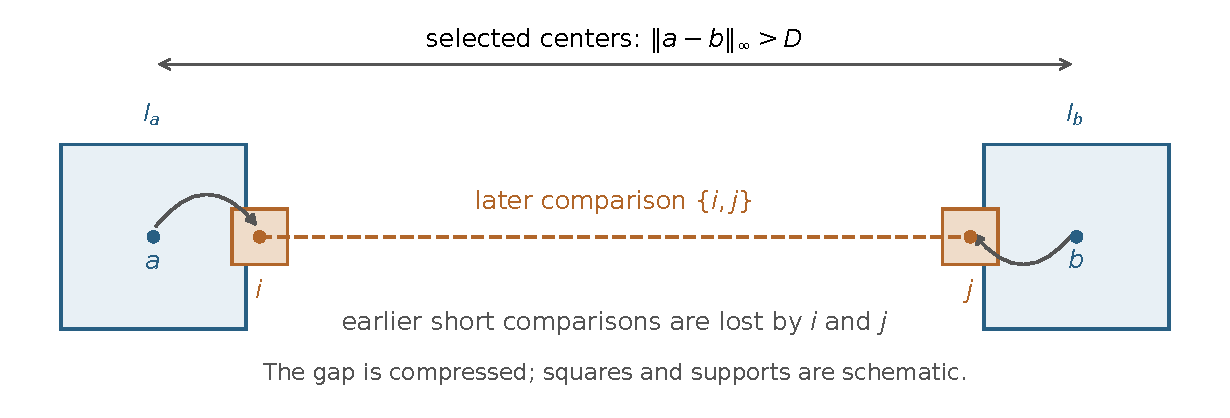
\includegraphics[width=\linewidth]{figures/separated-integrations.pdf}
 \caption{The geometry in Lemma~\ref{map:separated-integrations}, in
 parent units.  The orange supports meet the two selected squares.
 When $i\ne a$ and $j\ne b$, both endpoints have already lost a shorter
 comparison before the long comparison $\{i,j\}$.  If an endpoint
 equals its selected center, the proof uses the loss at the other
 endpoint.  Distances and support sizes are schematic; the separating
 gap is compressed.}
 \label{map:separation-figure}
\end{figure}

Given the new coins, collect all terms in
\eqref{map:coin-identity} meeting a selected $I_j$ into $H_j$.
Replace $H_j$ by
\begin{equation}\label{map:conditional-addition}
 \log\E_0[e^{H_j}\mid\text{field variables outside }I_j].
\end{equation}
All other terms remain.  The pure conditional laws in the selected
squares are independent given their exterior.  Lemma
\ref{map:separated-integrations} therefore shows, pointwise in the new
coins and exterior variables, that these replacements preserve the
integrated weight.  The output still contains every spin and old
auxiliary variable, together with the new coins; replacing the
logarithmic weight makes the updated old variables conditionally pure.
Their old law is recovered by the conditional tilt $e^{H_j}$.

Allocate a term in \eqref{map:conditional-addition} to its integration
parent.  Allocate untreated terms to their original parents, splitting
a pair term equally between its endpoints.  Fix these rules
symmetrically once and for all.  The allocated terms are functions of
the new coins as well as the remaining old field.  Center each by its
full-plane pure/reference mean.  The resulting potentials are denoted
$f'_j$.  Centering changes only a scalar partition factor, which can
depend on the environment but not on any field variable.

\begin{lemma}[Regular linearization]\label{map:linearization}
The regular map is analytic on a fixed supremum-norm neighborhood of
zero after $L$ is fixed.  Its derivatives of every prescribed finite
order are bounded uniformly in $s$ and depend on a bounded local
stencil of children.  Its first derivative is
\begin{equation}\label{map:linear-formula}
 f'_{j,\mathrm{lin}}
 =p^{-1}A_j\sum_{i\in\mathcal C_j}P^0_{I_j}f_i,
\end{equation}
where $P^0_{I_j}$ integrates the old reference field inside $I_j$.
The transferred sum is already centered.  In particular the linear
formula is independent of the reveal priorities.
\end{lemma}

\begin{proof}
Since $\E_eU_e=0$, every coin normalizer starts at degree two in the
child potentials.  The derivative of \eqref{map:conditional-addition}
at zero is conditional expectation.  These facts give
\eqref{map:linear-formula}.  Averaging the transfer in the full-plane
reference law gives zero by the centering of each child; averaging $A_j$
also preserves this centering.  On a small ball, real conditional
exponentials are uniformly bounded above and below.  The ordinary
power series for the exponential and logarithm consequently give the
asserted bounds in the supremum norm.  There are only finitely many
terms in each stencil, independently of $s$.
\end{proof}

\subsection{Large terms and isolated concentrations}

A moment estimate cannot assume that every realized potential is small.
We now modify the map where large child terms occur.  Fix $b>0$ and
independently attach to each child an environmental threshold uniform
on $[b,2b]$.  A child is a \emph{flag} if its norm exceeds its threshold.
The continuous thresholds will also make finite-step moment data
continuous in the initial coupling.

Declare a parent inactive when its center is within $10D$ parent units
of a flag.  In \eqref{map:coin-likelihood}, set its $F_j$ to zero and
retain its child terms separately.  Its coins remain as dummy
comparisons in the full local stars.  Active selected parents are
integrated as before.  Every retained term that involves an updated
interior variable is included in that integration; retained terms
supported entirely outside may simply be left in place.  Such a child
term has support much smaller than parent spacing and cannot meet two
selected squares.  Thus the same exact identity applies at the
boundary between active and inactive parents.

A further operation controls one isolated concentration of large terms.
Put $d_0=4C+10$.  An isolated group is a nonempty set $A$ of flags with
child-grid diameter at most $6d_0$ and with no flag outside $A$ within
$100D$ parent units of $A$.  Distinct such groups are separated.  Choose
one flag in $A$ using independent environmental priorities, and let
$j(A)$ be its parent.  Let
\[
 G_A=\sum_{i:\,\dist(i,A)\le3d_0}f_i,
 \qquad I_A=I_{j(A)}.
\]
Taking $L$ sufficiently large puts the support of $G_A$ deep inside
$I_A$.  All these children are in the inactive region.  No active
integration, or coin normalizer involving active old-field terms,
reaches $I_A$.

We remove $G_A$ while retaining all other interactions.  Let $B_A$ be
the sum of the remaining logarithmic terms that touch $I_A$.  With the
exterior fixed, replace $G_A$ by
\begin{equation}\label{map:isolated-ratio}
 R_A=\log\E_0[e^{B_A+G_A}\mid I_A^c]
       -\log\E_0[e^{B_A}\mid I_A^c].
\end{equation}
Here $I_A^c$ denotes all field variables not updated in $I_A$; new coins
are held fixed.  The identity
\begin{equation}\label{map:isolated-exactness}
 \E_0[e^{B_A+R_A}\mid I_A^c]
 =\E_0[e^{B_A+G_A}\mid I_A^c]
\end{equation}
proves that the exterior weight is unchanged.  The new conditional law
inside $I_A$ is tilted by $e^{B_A}$, and the old one by $e^{B_A+G_A}$.
In particular, retaining $B_A$ is part of the exact replacement.
Allocate $R_A$ to $j(A)$, and group all remaining terms at their parents.
These special integrations take priority over the preceding rule of
carrying inactive terms.  Their separation makes their order immaterial.

\begin{proposition}[The local scale map]\label{map:step}
There is a fixed support constant $C$ such that, for all sufficiently
large odd $L$ and every $b>0$, the preceding construction maps a field
with spacing $s$ and support/dependence radius $Cs$ to a field with
spacing $s'=Ls$ and support/dependence radius $Cs'$.  Its outputs are
centered, spin-flip even, stationary on the parent grid, and square
symmetric in distribution.  For a fixed numerical $K$ and a constant
$C_L$,
\begin{equation}\label{map:raw-bound}
 \|f'_j\|\le C_L\sum_{i:\,\|si-s'j\|_\infty\le Ks'}\|f_i\|.
\end{equation}
All replacements preserve exterior-integrated weights exactly, up to
the scalar constants removed by centering, and admit the reversals
described above.  The same formulas and centering constants apply in
embedded plane and torus charts.
\end{proposition}

\begin{proof}
Choose $C$ large enough to contain the comparison, inactivity, and
isolation ranges in parent units.  Then choose $L$ so large that old
supports overhang a parent by less than $1/10$ parent unit and
$100d_0/L<1/10$.  Every selection or status check, local allocation, and
conditional partition function then uses a fixed parent stencil.
Old environment dependence adds only an overhang $C/L$ in these units.
The new priorities and thresholds are independent and located in the
same stencil.  Increasing $C$ once, before fixing $L$, covers all these
supports.  No integration requires environment variables beyond the
terms that touch its finite square.

For any probability kernel $P$ and real bounded $H$,
$|\log Pe^H|\le\|H\|$.  The same inequality and its Lipschitz version
bound \eqref{map:conditional-addition} and
\eqref{map:isolated-ratio} by sums of the input norms.  The factors
$p^{-1}$ and the finite numbers of terms depend only on the fixed step.
Centering at most doubles this bound, proving \eqref{map:raw-bound}.
Spin flip commutes with every operation.  The symmetric choices and
allocation rules give the stated invariance in distribution.
Exactness follows from the normalized decoration,
\eqref{map:conditional-addition}, and
\eqref{map:isolated-exactness}.  Pure conditional kernels in an embedded
square depend only on its boundary assignment, so the same identities
hold on a torus.  We always subtract the same full-plane centering
constants, rather than torus means.
\end{proof}

\begin{corollary}[Local implementation]\label{map:locality}
In a finite free chart $W$ with arbitrary exterior field data, the map
can be performed away from its boundary so that the resulting
specification agrees with the full scale-$s'$ specification in
$W$ eroded by $K_1s'$, for a fixed numerical $K_1$.
\end{corollary}

\begin{proof}
Use the full local comparison stars.  If a parent's complete decoration
and allocation stencil leaves $W$, set its $F_j$ to zero in every $U_e$
and retain its original child logs separately.  Thus every fresh coin
with a nontrivial likelihood is inside $W$ and is sampled.  Skip integrations
whose stencils leave $W$.  Include retained terms in any
interior integration they meet.  Skip special integrations near the
boundary and keep active ones separated from them as above.  Every
operation affecting the eroded chart then uses precisely its full
stencil.  All remaining discrepancies are supported in the removed
boundary layer.  The argument applies also to annular charts.
\end{proof}

\subsection{Reversing the map and measuring finite insertions}

\begin{proposition}[A coupling of consecutive fields]\label{map:reversal}
For each fixed environment, the input and output spin fields of the
torus construction, or of the local construction with prescribed old
exterior field variables, can be
coupled so that they agree outside squares of radius $5s'$ about marked
parent centers.  The marks are mutually independent conditional on the
environment, independent of the output Gibbs sample, and have local
environmental parameters $p_j$ satisfying
\begin{equation}\label{map:mark-parameter}
 p_j\le\min\left\{1,C_L
       \sum_{i:\,\|si-s'j\|_\infty\le Ks'}\|f_i\|\right\}.
\end{equation}
For any $P\ge1$ and a stationary field with a finite $P$th environmental moment,
$\E p_j\le C_L(\E\|f_0\|^P)^{1/P}$.  These conclusions hold uniformly
over the old exterior assignments in the local implementation of
Corollary~\ref{map:locality}.
\end{proposition}

\begin{proof}
First sample the entire output Gibbs field, including the new coins.
Independently sample a uniform variable at every candidate parent
center, and mark $j$ when it is at most
$p_j=1-e^{-C_LS_j}$, with $S_j$ the environmental norm sum in
\eqref{map:mark-parameter}.  These parameters depend only on the
environment, so the marks have exactly the independence stated in the
proposition, before any further conditioning.

Condition now on the new coins and the common exterior of the updated
squares.  The ratio of the old conditional density to the new one is
bounded below by $e^{-C_LS_j}$, where $S_j$ is the local norm sum in
\eqref{map:mark-parameter}.  This follows from the real log bounds used
in Proposition~\ref{map:step}; for a special square it applies to the
tilt from $B_A$ to $B_A+G_A$.  If two laws satisfy
$\mu\ge(1-p)\nu$ and $p>0$, sample from $\nu$, retain that sample with probability
$1-p$, and otherwise sample from
$[\mu-(1-p)\nu]/p$.  The Bernoulli decision can be independent of the
$\nu$ sample; when $p=0$ the laws agree and the sample is retained.
Use this residual resampling in each marked updated square.  Conditional
factorization over the separated squares proves that the resampled
field has the old conditional law.  Unused centers keep their dummy
marks and cause no change.  Each update lies inside its radius-$5s'$ square.
Finally discard the conditionally decorated coins.  Their decoration
was normalized at each old field, so this recovers the input marginal.
Taking environmental expectation in \eqref{map:mark-parameter} gives
the last bound.
\end{proof}

One further consequence of exactness is needed for the variance
calculation.  For a finite family of labeled potentials at scale $s$,
define its normalized insertion density and charge by
\[
 D_f=\frac{\exp(\sum_i f_i)}{\E_0\exp(\sum_i f_i)},
 \qquad T_s(f)=q_s(D_f).
\]
The following statement concerns the regular map, before flags are
introduced, and therefore also its Taylor coefficients at zero.

\begin{corollary}[Charge of a finite insertion]\label{map:insertion-charge}
For every finite family of input labels, each fixed environment, and
each realization of the reveal priorities, the regular map satisfies
\[
 T_{Ls}(f')=L^{-1}T_s(f).
\]
The identity holds coefficientwise when separate indeterminates are
attached to the input labels.
\end{corollary}

\begin{proof}
Only a finite neighborhood of the insertion has nonzero decorations or
replacement terms.  Every observable outside a larger buffered region
has the same expectation against the normalized input and output
densities, because the decorations and replacements preserve its
unnormalized pairing and the partition function.  Apply this to a pure
bond tending to infinity.  Theorem~\ref{pure:charge} identifies the
limiting pairing with $Q$, so the total lattice charge is unchanged.
Dividing by the output scale $Ls$ instead of $s$ gives the factor
$L^{-1}$.  Scalar centering constants cancel in $D_f$.  Analyticity near
zero gives the coefficientwise assertion.
\end{proof}

\section{One-step moment bounds}\label{sec:moments}

We now estimate the local map in environmental moments.  The distinction
between the environmental mean and fluctuations is essential: the mean
has square symmetry and gains the stronger pure transfer exponent,
whereas centered fluctuations gain a square-root saving from finite
dependence.  Rare large terms require the isolated integrations of
Section~\ref{sec:local-map}.

Fix the even moment order $P=40$.  For a stationary scale-$s$ field, put
\begin{equation}\label{mom:coordinates}
 \begin{split}
 X&=(\E\|f_0\|^P)^{1/P},\qquad
 Y=\|\E f_0\|,\qquad m=\E q_s(f_0),\\
 W&=\sum_{i\in\Z^2}
       \Cov\bigl(q_s(f_0),q_s(f_i)\bigr).
 \end{split}
\end{equation}
All norms are supremum norms over field variables; expectations in
\eqref{mom:coordinates} are environmental.  Finite dependence makes
the covariance sum finite.  Moreover $W\ge0$: if $\Lambda$ is a growing
square of cell indices, then
\[
 \frac1{|\Lambda|}\Var\!\left(\sum_{i\in\Lambda}q_s(f_i)\right)
 \longrightarrow W.
\]
Primes will denote the same coordinates for the output field at scale
$Ls$, in particular $q_{Ls}=Q/(Ls)$.

\begin{proposition}[One-step estimates]\label{mom:one-step}
One can choose $L$ large, then $b>0$ small, and finally $x_*>0$ such that
for every input field of Section~\ref{sec:local-map} with $X\le x_*$,
\begin{equation}\label{mom:bounds}
 \begin{split}
 |m'-Lm|&\le C_LX^2,\\
 Y'&\le\rho Y+C_L(|m|+X^2),\\
 X'&\le\rho X+C_L(\sqrt W+Y),
 \end{split}
\end{equation}
where $\rho<1$ and all constants are independent of the scale $s$.
The constants denoted by $C_L$ may depend on all the fixed step
parameters, including the subsequently chosen $b$.
\end{proposition}

We first establish the fluctuation estimate for the linearized map.
It is useful to isolate the dimension-free moment fact that permits
us to take a supremum over an exponentially large spin boundary.

\begin{lemma}[Moments of finitely dependent Hilbert vectors]
\label{mom:hilbert}
Let $(V_i)_{i\in I}$ be centered random vectors in a real Hilbert space,
where $|I|=N$.  Suppose a graph of bounded degree on $I$ is a dependency
graph: subfamilies with no graph edge between them are independent.
Write $a=\max_i(\E\|V_i\|^P)^{1/P}$ and $S=\sum_iV_i$.  Then
\begin{equation}\label{mom:hilbert-bound}
 \E\|S\|^P
 \le C_P(\E\|S\|^2)^{P/2}
       +C_{P,\mathrm{dep}}N^{P/2-1}a^P.
\end{equation}
The constants do not depend on the dimension of the Hilbert space.
In particular,
$\|S\|_{L^P}\le C_{P,\mathrm{dep}}N^{1/2}a$.
\end{lemma}

\begin{proof}
Write $P=2r$ and expand
$\|S\|^{2r}=(\sum_{i,j}\langle V_i,V_j\rangle)^r$.
For each tuple of $2r$ occurrences, connect two occurrences when their
indices coincide or are neighbors in the dependency graph.  A singleton
component has expectation zero by centering and independence.  If all
components have size at least two and one has size greater than two,
there are at most $r-1$ components.  Bounded graph degree gives at most
$C_{P,\mathrm{dep}}N^{r-1}$ such tuples: choose one index per component,
then the remaining indices along a spanning tree.  H\"older's inequality
bounds each expectation in absolute value by $a^{2r}$.

For the remaining tuples every component is a pair.  Independence
factors their expectation into contractions of pair covariance
operators.  Sum these contractions over all pairings and allow the
indices belonging to different pairs to be adjacent.  The added tuples
have merged components and incur the same
$C_{P,\mathrm{dep}}N^{r-1}a^{2r}$ error.  The unrestricted sum is exactly
the Wick expression for $\E\|Z\|^{2r}$, where $Z$ is a centered Gaussian
Hilbert vector with the covariance operator of $S$.  This operator is
positive even though individual cross-covariances need not be positive.
Diagonalizing it gives
$\E\|Z\|^{2r}\le C_P(\E\|Z\|^2)^r
=C_P(\E\|S\|^2)^r$.  Finite-dimensional projection and monotone
convergence give the same conclusion in a general Hilbert space.
Finally bounded dependence gives
$\E\|S\|^2\le C_{\mathrm{dep}}Na^2$.
\end{proof}

\subsection{Fluctuations of the linear map}

Fix a parent, translated to the origin, and transfer first to the
boundary of the square of radius $3Ls$.  Take the Hilbert norm there
with respect to the pure full-plane boundary marginal.  The pure
buffered density comparison, as stated in
\cite[Section~2, Proposition ``Buffered and small-patch comparisons'']{S},
bounds the final conditional transfer from this boundary to
$\partial I_0$ in supremum norm by a fixed constant times the Hilbert
norm.  Thus random Hilbert sums control the supremum in
\eqref{map:linear-formula}; the factor $p^{-1}A_0$ costs at most $p^{-1}$.
This factor is fixed independently of $L$.

Let
\[
 g_i=f_i-\E f_i,\qquad t_i=q_s(g_i).
\]
Choose the bounded energy representatives
$e_i=sP_{Cs,si}B_{si}$, enlarging the fixed support constant if necessary;
$B_{si}$ is the bond average of Theorem~\ref{pure:charge} at $si$,
and the transfer is through a square centered there.
Then $Q(e_i)=s$, $q_s(e_i)=1$, and $\|e_i\|\le C$.
Decompose
\[
 g_i=h_i+t_ie_i,\qquad Q(h_i)=0.
\]
Both $h_i$ and $t_i$ are centered in the environment, and
$\|h_i\|_{L^P(\E;\infty)}+\|t_i\|_{L^P(\E)}\le CX$.

The transferred $h_i$ have supremum norm at most
$CL^{-u}\|h_i\|$, by Theorem~\ref{pure:charge}.  One may first
transfer across a square centered at the child and then condition onto
the intermediate parent boundary.  There are $L^2$ children, with a
fixed dependence range in child units.  Lemma~\ref{mom:hilbert} bounds
their sum in $L^P(\E;L^2)$ by
\begin{equation}\label{mom:stable-fluctuation}
 CL^{1-u}X.
\end{equation}

For the charge part, let $w_i$ be the transfer of $e_i$ to the same
intermediate boundary.  These are deterministic Hilbert vectors with
\begin{equation}\label{mom:energy-vectors}
 \|w_i\|\le C/L,\qquad
 \|w_i-w_j\|\le CL^{-u}
 \quad\text{if }\|i-j\|_\infty\le2C.
\end{equation}
For the second estimate, $e_i-e_j$ has zero charge and is supported in
a fixed enlargement of one child neighborhood, so the zero-charge
transfer estimate applies.

Here the total covariance $W$ gives a sharper bound than the variance
of a single child.  Put $c(h)=\Cov(t_0,t_h)$ and let
$I=\mathcal C_0$.  Stationarity and finite dependence give the identity
\begin{align}
 \E\left\|\sum_{i\in I}t_iw_i\right\|^2
 &=W\sum_{i\in I}\|w_i\|^2\notag\\
 &\quad+\sum_{\substack{i\in I,h\\i+h\in I}}
 c(h)\langle w_i,w_{i+h}-w_i\rangle
 -\sum_{\substack{i\in I,h\\i+h\notin I}}c(h)\|w_i\|^2.
 \label{mom:covariance-regrouping}
\end{align}
Only a fixed number of $h$ contribute, and $|c(h)|\le CX^2$.
The first term is at most $CW$ because $W\ge0$ and
$\sum_i\|w_i\|^2\le C$.  By \eqref{mom:energy-vectors}, the second term
is $O(L^{1-u}X^2)$.  The last term has only $O(L)$ indices $i$ within
a fixed distance of the block boundary, so it is $O(L^{-1}X^2)$.
Consequently
\begin{equation}\label{mom:charge-variance}
 \E\left\|\sum_{i\in I}t_iw_i\right\|^2
 \le CW+C(L^{1-u}+L^{-1})X^2.
\end{equation}
Applying Lemma~\ref{mom:hilbert} with $N=L^2$ and $a=CX/L$ gives
\begin{equation}\label{mom:charge-P}
 \left\|\sum_{i\in I}t_iw_i\right\|_{L^P(\E;L^2)}
 \le C\sqrt W+
 C\bigl(L^{(1-u)/2}+L^{-1/2}+L^{-2/P}\bigr)X.
\end{equation}
The bound has no dependence on the dimension of the spin boundary.
Together with \eqref{mom:stable-fluctuation} and the final buffered
transfer, it implies
\begin{equation}\label{mom:linear-fluctuation}
 \|f'_{0,\mathrm{lin}}(f-\E f)\|_{L^P(\E;\infty)}
 \le\eta_LX+C\sqrt W,
 \qquad \eta_L\longrightarrow0.
\end{equation}
All constants in the limit statement use only the support range and
$p$, fixed before $L$.

\subsection{Charge, mean, and small Taylor remainders}

The exact normalization of $Q$ makes the first line of
\eqref{mom:bounds} especially simple.  Applying $q_{Ls}$ to
\eqref{map:linear-formula} integrates the new selection coins, so that
$p^{-1}$ cancels $\E_0A_j=p$.  Charge is preserved by pure transfer.
Therefore
\begin{equation}\label{mom:linear-charge}
 \E q_{Ls}(f'_{0,\mathrm{lin}})
 =\frac1L\sum_{i\in\mathcal C_0}\E q_s(f_i)=Lm.
\end{equation}

For the environmental mean, let
$\bar f_i=\E_{\mathrm{aux}}\E f_i$, where the auxiliary expectation
uses their independent reference law and leaves the spins fixed.
Then $\|\bar f_i\|\le Y$ and $q_s(\bar f_i)=m$.
The deterministic spin function $\bar f_i$ is quarter-turn invariant
about its center, because both the environmental distribution and the
auxiliary reference law respect this symmetry.  The transfer inside
$I_0$ integrates all these old auxiliary variables, so its mean is
the transfer of $\bar f_i$.  Subtract $m e_i$ from $\bar f_i$.
The difference has zero charge and norm at most $CY$,
since $|m|\le CY$.  Its transfer costs $CL^{-w}Y$ per child.  The charge
part costs $C_L|m|$.  Thus
\begin{equation}\label{mom:linear-mean}
 \|\E f'_{0,\mathrm{lin}}\|
 \le CL^{2-w}Y+C_L|m|.
\end{equation}
For use in the last line of \eqref{mom:bounds}, the simpler general
transfer bound also gives
\begin{equation}\label{mom:linear-total}
 \|f'_{0,\mathrm{lin}}\|_{L^P(\E;\infty)}
 \le\eta_LX+C_L(\sqrt W+Y).
\end{equation}

We record how flagged stencils affect low moments.  Enlarge a parent
stencil to include every comparison, threshold, and isolation check
that can affect its output, and put $S=\sum_{i\in\mathcal S}\|f_i\|$.
Its size depends only on the fixed step.  Let $\mathcal B$ be the event
that it contains a flag.  Markov's inequality and H\"older give
\begin{equation}\label{mom:bad-low-moments}
 \Prob(\mathcal B)\le C_{L,b}X^P,
 \qquad \E[S^r\1_{\mathcal B}]\le C_{L,b}X^P
 \quad(1\le r\le P).
\end{equation}
For example, for $r<P$ the second bound follows from
$(\E S^P)^{r/P}\Prob(\mathcal B)^{1-r/P}$; for $r=P$ it is immediate.
Choose $b$ after $L$ so small that $2|\mathcal S|b$ lies in the uniform
Taylor neighborhood of Lemma~\ref{map:linearization}.  If there is no
flag, every child norm is at most $2b$, and the regular Taylor remainder
$R$ satisfies
\begin{equation}\label{mom:regular-remainder}
 \|R\|\le C_LS^2\le C_LbS.
\end{equation}
In the second inequality the constant is independent of $b$.
The raw bound \eqref{map:raw-bound} and
\eqref{mom:bad-low-moments} show that the actual map differs from its
linearization by $O_L(X^2)$ in first environmental moment.  Equations
\eqref{mom:linear-charge} and \eqref{mom:linear-mean}, together with the
charge norm bound of Theorem~\ref{pure:charge}, now prove the first
two lines of \eqref{mom:bounds}, once $L$ is large enough that
$CL^{2-w}<1$.

The same reasoning does not yet prove a contraction in the $P$th
moment: the bound for $r=P$ in \eqref{mom:bad-low-moments} has size
$X^P$, not a higher power.  The next argument uses the location of the
flags to recover a small factor.

\subsection{The contribution of isolated large terms}

Consider one contributing child log $f_i$ in the raw output stencil
of \eqref{map:raw-bound}.  Enlarge the determining stencil to contain
the child-grid square of radius $100DL+2C$ about each such index $i$,
as well as every status check that can affect the output.  In particular,
this enlargement contains the full isolation neighborhood of any flag
group lying within $2C$ of a contributing log.  If a flag in this stencil
$k$ has $\|i-k\|_\infty>2C$, then $f_i$ is independent of that flag,
including its fresh threshold.  Hence
\begin{equation}\label{mom:independent-flag}
 \E[\|f_i\|^P\1_{\{k\text{ is a flag}\}}]
 =\E\|f_i\|^P\,\Prob(k\text{ is a flag})
 \le C_bX^{2P}.
\end{equation}
A union bound over the fixed enlarged stencil makes all such
contributions $O_{L,b}(X^2)$ in $P$th-root norm.

It remains to consider contributions for which every flag in this stencil
lies within $2C$ of $i$.  The flags then have diameter at most $4C$.
The inclusion of the full isolation neighborhoods ensures that they
form an isolated group of the construction.  All logs that can depend
on these flags lie within the $3d_0$ neighborhood transferred as $G_A$.
Equivalently, if isolation fails because of a distant additional flag,
that flag is independent of the contributing log and
\eqref{mom:independent-flag} applies.  This is the needed dichotomy;
small flag probability alone would not suffice.

For the isolated group, compare \eqref{map:isolated-ratio} with the
same expression after the other touching logs $B_A$ have been removed.
For every probability kernel $P_0$,
\begin{equation}\label{mom:remove-background}
 \left|\log\frac{P_0e^{B_A+G_A}}{P_0e^{B_A}}
                  -\log P_0e^{G_A}\right|
 \le2\|B_A\|.
\end{equation}
Each child log in $B_A$ lies outside the group neighborhood and is
independent of an actual triggering flag.  On the event that this group
occurs, its $P$th-root contribution is therefore $O_{L,b}(X^2)$ by
\eqref{mom:independent-flag}.  The same is true for every other log
omitted from the concentrated contribution.

After this removal, Lemma~\ref{pure:positive-weight} gives
\begin{equation}\label{mom:isolated-contraction}
 \left\|\log\E_0[e^{G_A}\mid I_A^c]
       -\E_0\log\E_0[e^{G_A}\mid I_A^c]\right\|
 \le \frac{C}{L}\sum_{i:\,\dist(i,A)\le3d_0}\|f_i\|.
\end{equation}
Indeed $G_A$ lies in a patch of radius a fixed multiple of $s$.
If this patch is not concentric with $I_A$, first transfer to the square
of radius $2Ls$ about the representative flag, which is contained in
$I_A$, and then condition onward.  Averaging a positive density cannot
increase its log oscillation.  Centering increases the oscillation
bound by at most a fixed factor.

There are a bounded number of possible flag patterns within a fixed
child-radius neighborhood of an anchor, and $O(L^2)$ possible anchoring
children for a given output stencil.  Separation bounds the number of
simultaneous isolated groups in that stencil by a constant independent
of $L$.  Raising \eqref{mom:isolated-contraction} to the $P$th power,
using the bounded number of logs in each group, and summing over anchors
therefore gives
\begin{equation}\label{mom:outlier-output}
 \|\1_{\mathcal B}f'_0\|_{L^P(\E;\infty)}
 \le CL^{2/P-1}X+C_{L,b}X^2.
\end{equation}
The first constant uses only the fixed child support radius; in
particular it is independent of $L$ and $b$.  This counting may be done
without disjointness of the anchoring events: use their union bound
before taking the $P$th root.

For completeness the linear output on the same event satisfies the
same bound, with a possibly different fixed constant.  Charge each
child term to a flag farther than $2C$ whenever one is present and use
\eqref{mom:independent-flag}.  Otherwise only a bounded child-radius
cluster can contribute a dependent large term.  The ordinary even
transfer to the parent boundary costs $C/L$ for that cluster.  The same
$O(L^2)$ anchor count then gives
\begin{equation}\label{mom:outlier-difference}
 \|\1_{\mathcal B}(f'_0-f'_{0,\mathrm{lin}})\|_{L^P(\E;\infty)}
 \le CL^{2/P-1}X+C_{L,b}X^2.
\end{equation}
Fixed multiplicities from the allocation of terms are included in the
constants.

\begin{proof}[Completion of Proposition~\ref{mom:one-step}]
The last line follows by combining \eqref{mom:linear-total},
\eqref{mom:regular-remainder}, and
\eqref{mom:outlier-difference}:
\[
 X'\le\bigl(\eta_L+CL^{2/P-1}+C_Lb\bigr)X
       +C_{L,b}X^2+C_L(\sqrt W+Y).
\]
Choose $L$ large enough that the first two coefficients, and the
coefficient $CL^{2-w}$ in \eqref{mom:linear-mean}, leave a strict margin
below one.  This is possible because $u>1$, $w>2$, and $P>2$.
Choose $b$ next to put flag-free stencils in the Taylor neighborhood
and make $C_Lb$ smaller than the remaining margin.  Finally choose
$x_*$ so that $C_{L,b}X$ is smaller than that margin for $X\le x_*$.
Increasing the resulting contraction factor to one common $\rho<1$
proves all three assertions.
\end{proof}

The mark parameters in Proposition~\ref{map:reversal} consequently
satisfy $\E p_j\le C_LX$.  We also record the precise Taylor consequence
needed below.

\begin{corollary}[Fourth-order moment substitution]
\label{mom:taylor-substitution}
Fix finitely many output stencils and a bounded multilinear expression
in at most four output potentials in total, allowing pure expectations,
environmental expectations, and products of such expectations.
The multilinear kernels are uniformly bounded in the scale; constants
may depend on these kernels and their fixed stencils.
Substitute the regular map's Taylor polynomial through degree four
and retain only total input degree at most four.  The resulting
environmental moment differs from that of the actual map by
$O_L(X^5)$, uniformly in $s$.
\end{corollary}

\begin{proof}
On the unflagged stencils, the fifth-order Taylor remainder and
H\"older's inequality give $O_L(X^5)$.  On flagged stencils use the
raw bound for the actual outputs and
\eqref{mom:bad-low-moments}.  Products of four fourth-order Taylor
polynomials have degree at most $16<P$, so the same bound controls
every term there.  Terms of input degree between five and sixteen
have expectation $O_L(X^5)$ when $X\le1$.  Products of separately
taken expectations obey the identical estimates.
\end{proof}

\section{A variance coordinate and its marginal decay}
\label{sec:variance}

The estimates of Proposition~\ref{mom:one-step} leave one quantity
uncontracted: the variance density $W$ of the energy charges.  We now
replace $W$ by a polynomial coordinate whose leading change under one
scale step is a negative multiple of $W^2$.  The normalization of a finite insertion
is responsible for that sign.

The coordinate's quadratic part will be exactly $W$.  In a product of
two independent centered insertions, the normalizing denominator first
affects the variance at degree four; its distant energy contribution
is negative.  Including the local cubic and quartic insertion
coefficients makes this calculation compatible with an exact scale
step.  We define those coefficients before computing their change.

Throughout this section the spacing is $s$, and $q_s=Q/s$.  All input
potentials are centered under the pure reference law $\E_0$, which
includes the auxiliary variables.  Environmental expectation $\E$ does
not integrate these auxiliary variables; it does integrate the independent
priorities and thresholds used to construct the scale map.  Write $R_0$
for a fixed dependence range in cell units, enlarged so that disjoint
sets of cells at distance greater than $R_0$ use disjoint environment
variables and have disjoint declared supports.

\subsection{Normalized insertion coefficients}

For a finite set of cell indices $I$ and real indeterminates
$\mathbf t=(t_i)_{i\in I}$, set
\begin{equation}
 F_I(\mathbf t)=\sum_{i\in I}t_i f_i,
 \qquad
 \mathcal T_I(\mathbf t)
 =q_s\left(\frac{e^{F_I(\mathbf t)}}{\E_0e^{F_I(\mathbf t)}}\right).
 \label{var:insertion}
\end{equation}
For each fixed environment these expressions are analytic near the
origin.  We use only their Taylor coefficients, so no exponential
integrability with respect to the environment is required.  In
particular, since $\E_0F_I=0$ and $q_s$ kills constants, the first three
homogeneous terms are
\begin{align}
 \mathcal T_1(F)&=q_s(F),&
 \mathcal T_2(F)&=\tfrac12q_s(F^2),\notag\\
 \mathcal T_3(F)&=\tfrac16q_s(F^3)
       -\tfrac12q_s(F)\E_0F^2.
 \label{var:charge-expansion}
\end{align}
Consequently the terms of degrees two, three, and four in the
environmental variance of $\mathcal T_I$ are, respectively,
\begin{equation}
 \Var(\mathcal T_1),\qquad
 2\Cov(\mathcal T_1,\mathcal T_2),\qquad
 \Var(\mathcal T_2)+2\Cov(\mathcal T_1,\mathcal T_3).
 \label{var:variance-expansion}
\end{equation}
All covariances in this section are environmental unless a subscript
$0$ is present.

Here is an explicit convention for the coefficients, including repeated
indices.  For an ordered tuple $\boldsymbol i=(i_1,\ldots,i_d)$, give
its $d$ occurrences separate indeterminates $t_1,\ldots,t_d$, even
when some $i_a$ coincide.  Define the symmetric multilinear coefficient
\begin{equation}
 C_d(\boldsymbol i)=
 \left.
 \partial_{t_1}\cdots\partial_{t_d}
 \Var\left[
 q_s\left(\frac{\exp(\sum_{a=1}^d t_a f_{i_a})}
                   {\E_0\exp(\sum_{a=1}^d t_a f_{i_a})}\right)
 \right]\right|_{\mathbf t=0},
 \qquad 2\le d\le4.
 \label{var:polarized-coefficient}
\end{equation}
The derivative in this formula means coefficient extraction using
\eqref{var:charge-expansion}--\eqref{var:variance-expansion}; thus it
is a finite sum of moments.  In particular its definition remains valid
when the random potentials have only the finite moments assumed in
Section~\ref{sec:moments}.

\begin{definition}[Variance coordinate]\label{var:coordinate}
For $H>R_0$, define
\begin{equation}
 v_H=\sum_{d=2}^4\frac1{d!}
 \sum_{i_2,\ldots,i_d\in\Z^2}
 \1_{\{\diam(0,i_2,\ldots,i_d)\le H\}}
 C_d(0,i_2,\ldots,i_d).
 \label{var:coordinate-formula}
\end{equation}
The diameter is Euclidean diameter in cell units.  The coordinate is
real and need not be nonnegative for an arbitrary field.
\end{definition}

The factorial and the ordered slots in
\eqref{var:coordinate-formula} are the usual Taylor convention.  An
equivalent definition sums over all ordered tuples in a large cell box,
divides by the number of cells, and takes the limit.  Stationarity and
the finite diameter cutoff give this equivalence.  This latter definition
also applies when an intermediate allocation is periodic on parent
cells: average over complete parent periods before passing to the limit.

\begin{lemma}\label{var:near-W}
For each fixed $H>R_0$, there is $C_H<\infty$, independent of $s$,
such that
\begin{equation}
 |v_H-W|\le C_H X^3\qquad\text{if }X\le1.
 \label{var:near-W-bound}
\end{equation}
\end{lemma}
\begin{proof}
The quadratic coefficient is
$C_2(i,j)=2\Cov(q_s(f_i),q_s(f_j))$.  Its contribution is therefore
exactly $W$, because covariances vanish past the dependence range.
Every remaining coefficient has three or four potential occurrences.
Their supports fit in a ball of radius $O(Hs)$.  The charge bound in
Theorem~\ref{pure:charge}, the boundedness of pure expectation, and
H\"older's inequality bound each coefficient of degree $d$ by
$C_H X^d$.  There are finitely many tuples with first slot zero and
diameter at most $H$.
\end{proof}

\subsection{The change of cutoff}

We first change $H$ to $LH$ without changing the field.  This calculation
contains the sign of the flow.  Later we compare this larger cutoff with
the coordinate of the output field.

\begin{lemma}[Shell calculation]\label{var:shell}
Fix finite constants $A,B$.  If $0<z\le1$, $X\le Az$, and
$Y\le Bz^2$, then
\begin{equation}
 v_{LH}-v_H
 =-2\kappa W^2\sum_{y\in\Z^2:\ H<|y|\le LH}|y|^{-2}
   +e_H z^4+O_H(z^5),
 \label{var:shell-formula}
\end{equation}
where $|e_H|$ is bounded by a deterministic function tending to zero
as $H\to\infty$.  The constants may depend on $A,B$ and the fixed
scale-step parameters, but are uniform in $s$.
\end{lemma}
\begin{proof}
Decompose $f_i=\bar f_i+\widetilde f_i$, where
$\bar f_i=\E f_i$.  An occurrence of $\widetilde f_i$ has size order
one, and an occurrence of $\bar f_i$ has size order two.  Products
of total size order at least five contribute $O_H(z^5)$ by
H\"older's inequality.  For the remaining coefficients connect two
occurrences when their cell indices are within $R_0$.  A connected
component containing at most four occurrences has bounded diameter.
Moreover, a component consisting of a single centered occurrence
has zero environmental expectation in every term of the covariance
expansion.  Thus, once $H$ is large, a nonzero coefficient in the shell
has precisely two distant groups: either a centered pair and one mean,
or two centered pairs.  Each has total size order four.  This argument
applies also to the products of means subtracted in a covariance.

Call the two groups $A$ and $B$.  Let $1+g_A$ and $1+g_B$ be their
separately normalized insertion densities, expanded formally in their
own indeterminates.  Every coefficient of $g_A,g_B$ is pure centered.
Define
\begin{equation}
 T_A=q_s(g_A),\quad T_B=q_s(g_B),\quad
 h_{AB}=q_s(g_Ag_B),\quad c_{AB}=\E_0(g_Ag_B).
 \label{var:two-group-quantities}
\end{equation}
Multiplying the two densities and normalizing again gives the exact
formal identity
\begin{equation}
 \mathcal T_{A\cup B}
       =\frac{T_A+T_B+h_{AB}}{1+c_{AB}}.
 \label{var:two-group-identity}
\end{equation}
If the anchor distance is $l$, Proposition~\ref{pure:fusion} gives,
coefficient by coefficient,
\begin{equation}
 h_{AB}=O(l^{-u}),\qquad
 c_{AB}=l^{-2}\bigl(\kappa T_AT_B+o(1)\bigr).
 \label{var:cross-coefficient-bounds}
\end{equation}
The estimates carry the product of the norms of the local coefficient
functions.  All group diameters are bounded, so their constants are
uniform in the slots and in $s$.

The variance of $T_A+T_B$ has no coefficient using both independent
groups.  Contributions with two cross factors $h_{AB}$ or $c_{AB}$
have shell sum bounded by $C H^{2-2u}z^4=o_H(1)z^4$.  For a single
$h_{AB}$ we use the stronger, symmetric part of
Proposition~\ref{pure:fusion}.  To justify its applicability, first
replace the cutoff on total diameter by the cutoff on anchor distance
and sum all bounded relative positions inside each group.  Environmental
factorization turns the required coefficient into a finite sum of
bilinear charge pairings of deterministic functions.  More explicitly,
the two possible local sums, besides $\bar f_x$, are
\begin{align*}
 D_x&=\sum_{|a|\le R_0}
       \E\bigl[q_s(\widetilde f_x)\widetilde f_{x+a}\bigr],\\
 M_x&=\sum_{|a|\le R_0}
       \E\bigl[\widetilde f_x\widetilde f_{x+a}
                   -\E_0(\widetilde f_x\widetilde f_{x+a})\bigr].
\end{align*}
The pair-plus-mean sector gives pairings $q_s(D_x\bar f_y)$;
the pair-plus-pair sector gives $q_s(D_xM_y)$, with their exchanges
and the fixed scalar factors from Taylor expansion.  This list follows
by taking the linear charge from one group and the term linear in that
group in $h_{AB}$; the other group supplies its mean or its quadratic
normalized density.  Terms leaving a centered singleton vanish as
above.  All displayed functions are pure centered, and $D_x,M_x$
have norm $O(z^2)$.  Rotation of the offset sum preserves both its
index set and the environment law, while charge is a rotation-invariant
scalar.  Thus each function is quarter-turn invariant about its anchor.
The resulting bound is
$C l^{-w}z^4$, whose shell sum is $O(H^{2-w})z^4=o_H(1)z^4$.

The replacement of diameter by anchor distance affects only strips
of bounded thickness at the two ends of the shell.  There are $O(H)$
possible anchor displacements in these strips, and the unsymmetrized
bound $O(H^{-u})$ gives an error $O(H^{1-u})z^4$.  Thus the replacement
and its reversal both have vanishing error as $H\to\infty$.

Only the single-$c_{AB}$ contribution remains.  Up to size order four
it is
\begin{equation}
 -2\Cov\bigl(T_A+T_B,(T_A+T_B)c_{AB}\bigr).
 \label{var:normalization-term}
\end{equation}
Its four occurrences must all be centered; a mean would increase
the size order.  Write $U=T_{A,1}$ and $V=T_{B,1}$.  These are
independent centered random scalars.  At bidegree $(2,2)$,
\begin{align}
 -2\Cov(U+V,(U+V)\kappa l^{-2}UV)
 &=-2\kappa l^{-2}\E[(U+V)^2UV]\notag\\
 &=-4\kappa l^{-2}\E U^2\E V^2.
 \label{var:quartic-sign}
\end{align}
The $o(1)$ in \eqref{var:cross-coefficient-bounds} gives
$o_H(1)z^4$ after shell summation, since $L$ is fixed and
$\sum_{H<|y|\le LH}|y|^{-2}$ is bounded.

We finally spell out the slot count.  Put
$a_{ij}=\Cov(q_s(f_i),q_s(f_j))$.  Suppose the four labeled slots
split into the far pairs $\{1,2\}$ and $\{3,4\}$.  The coefficient
of $t_1t_2$ in $\E U^2$ is $2a_{i_1i_2}$, even when the two cell
indices coincide; the occurrences still have distinct indeterminates.
The other pair contributes $2a_{i_3i_4}$.  Hence the polarized
normalization contribution is
\[
 -16\kappa |i_3-i_1|^{-2}a_{i_1i_2}a_{i_3i_4}.
\]
There are three partitions of four labeled slots into two unordered
pairs.  Their sums agree by permutation of the dummy slots, and a
tuple in a sufficiently distant shell has at most one such far
pairing.  The prefactor from \eqref{var:coordinate-formula} is
$1/4!$, so the numerical coefficient is
$-16\cdot3/4!=-2$.  For the pairing just displayed, anchoring
$i_1=0$ and writing $y=i_3$ gives
\[
 \sum_{i_2}a_{0i_2}\sum_{i_4}a_{y i_4}=W^2.
\]
Both sums are finite, and stationarity makes the second equal to $W$.
Changes of the cutoff caused by bounded shifts of anchors have the
strip bounds already proved.  A change of anchor in the kernel itself
also has vanishing error: for bounded $\delta$ and $|y|\asymp H$,
$\bigl||y+\delta|^{-2}-|y|^{-2}\bigr|\le C|\delta|H^{-3}$,
whose shell sum is $O(H^{-1})$.  This proves
\eqref{var:shell-formula}.
\end{proof}

\subsection{Passing to the output coordinate}

Let $f'_j$ be the output potentials at spacing $Ls$, and let $v'_H$
be their coordinate.  A finite insertion has the same exterior marginal
before and after the regular scale map.  The next argument explains why
this identity applies to the truncated, locally allocated coordinate.

\begin{lemma}[Compatibility of the coordinate]\label{var:compatibility}
Under the hypotheses of Lemma~\ref{var:shell},
\begin{equation}
 v'_H-v_{LH}=e_Hz^4+O_H(z^5),
 \label{var:compatibility-bound}
\end{equation}
with the same uniformity convention for $e_H$.
\end{lemma}
\begin{proof}
First use the regular map and retain the child indeterminates.  For
finitely many labeled inputs its normalized total insertion charge
obeys
\begin{equation}
 \mathcal T_{\mathrm{out}}=L^{-1}\mathcal T_{\mathrm{in}}
 \label{var:total-charge-preservation}
\end{equation}
by Corollary~\ref{map:insertion-charge}.  One can also see the normalization
directly: the conditional coin likelihood integrates to one at every
fixed old configuration, and each conditional integration preserves
pairing with a test outside the affected region.  Pairing with a distant
pure bond identifies $Q$ by Theorem~\ref{pure:charge}.  Centering
the allocated output logs changes only a scalar, which disappears from
the normalized insertion.  The factor $L^{-1}$ in
\eqref{var:total-charge-preservation} is exactly the change from $Q/s$
to $Q/(Ls)$.

This argument holds for every fixed realization of the fresh priorities.
Taking environmental variance and then Taylor coefficients therefore
preserves complete coefficients, including their mean subtractions.
The variance factor $L^{-2}$ cancels the $L^2$ children per parent
when sums are taken per unit area.  If an allocation distinguishes
positions within a parent, take the area average over complete parent
periods.  There is no assumption of invariance of individual allocated
coefficients under child translations.

We must compare the two cutoffs.  Every output Taylor coefficient uses
children in a fixed stencil.  Thus classifying a coefficient by parent
diameter $H$ rather than child diameter $LH$ changes its classification
only when the child diameter lies in a strip of width $O_L(1)$ about
$LH$.  Keep together the full covariance coefficient for each fixed
tuple of output arguments, including all its mean subtractions, and
only then expand its arguments in child slots.  The parent cutoff
is constant on precisely this grouping.  More explicitly, write
$R_j$ for the regular output at parent $j$, as a function of its
child potentials.  A Taylor contribution with $m$ output arguments
and child degree $d$, where $2\le m\le d\le4$, assigns its $d$
occurrence slots to nonempty blocks $B_1,\ldots,B_m$ and
uses the random functions
\begin{equation}
 G_a=D^{|B_a|}R_{j_a}(0)
        [f_{i_b}:b\in B_a],\qquad 1\le a\le m.
 \label{var:taylor-blocks}
\end{equation}
The directions in this derivative are supported at their indicated
child labels; repeated labels are allowed.  Multilinear substitution
gives the complete polarized covariance coefficient of
$G_1,\ldots,G_m$, with its Taylor factors and the single common
weight $\1_{\{\diam(j_1,\ldots,j_m)\le H\}}$.

Discard size orders at least
five, at cost $O_H(z^5)$, and connect child slots when their enlarged
stencils can share environment variables.  A singleton centered child
has zero expectation even conditional on
the fresh priorities: the Taylor kernel depends on those independent
priorities and takes the child function as a multilinear argument.
A singleton mean costs size order two.  Two components containing means
only cannot create a lower-order term through random allocation.  At the
only relevant order their output is the linear map of
Lemma~\ref{map:linearization}, which is independent of priorities;
its selection indicators are reference auxiliary variables, integrated
by $Q$.  In particular its charges are deterministic when its inputs
are deterministic.  We are therefore left with two distant components
of bounded diameter and size order two each.

Every output argument receiving a child slot lies in that slot's
bounded stencil.  These components consequently partition the relevant
output arguments into two distant groups as well: each block $B_a$
in \eqref{var:taylor-blocks} lies wholly in one component.  Apply
\eqref{var:two-group-identity} to the two finite lists of output
arguments $G_a$, with separate insertion indeterminates $u_a$.
The groups are
independent in the environment, including their fresh priorities.
For their separate charges the formal identity
\[
 \Var\bigl(T_A(\mathbf u_A)+T_B(\mathbf u_B)\bigr)
 =\Var T_A(\mathbf u_A)+\Var T_B(\mathbf u_B)
\]
has zero coefficient involving variables from both groups, regardless
of their separate means.  Thus the unmixed contribution cancels for
each fixed output tuple and each child-block partition, before any
sum over output labels.  Repeated child labels merely repeat derivative
directions inside a group; no within-group independence is used.
The remaining terms have a cross factor and hence
an $O_L(H^{-u})$ bound from Proposition~\ref{pure:fusion}.
The strip therefore costs
$O_L(H^{1-u})z^4=o_H(1)z^4$.  Keeping the covariance subtractions with
each coefficient is essential here and is permitted because the cutoff
depends only on the tuple of labels.

Finally apply Corollary~\ref{mom:taylor-substitution}.  For each fixed
output tuple, \eqref{var:variance-expansion} is a sum of bounded
multilinear expressions in at most four output potentials, including
products of separately taken expectations.  The charge bound on its
fixed-$H$ support makes the kernels uniformly bounded in $s$.  The
corollary applies to the finite union of all determining stencils,
including their status checks.  It therefore replaces the regular
Taylor output by the actual output and removes child degrees above
four with total error $O_H(X^5)=O_H(z^5)$.  In particular the highest
intermediate degree is $4\cdot4=16<P=40$, so the finite moment
assumption suffices.  This proves \eqref{var:compatibility-bound}.
\end{proof}

\begin{proposition}[Marginal variance flow]\label{var:flow}
Fix the scale-step parameters and finite constants $A,B$.  For every
sufficiently large fixed $H$, the polynomial coordinate of
Definition~\ref{var:coordinate} satisfies, whenever
$0<z\le1$, $X\le Az$, and $Y\le Bz^2$,
\begin{equation}
 v'_H-v_H
 =-2\kappa W^2\sum_{y\in\Z^2:\ H<|y|\le LH}|y|^{-2}
   +e_Hz^4+O_H(z^5),
 \label{var:flow-formula}
\end{equation}
where $|e_H|\to0$ as $H\to\infty$, uniformly in the lattice scale.
Moreover $|v_H-W|\le C_HX^3$ for $X\le1$.
\end{proposition}
\begin{proof}
Combine Lemmas~\ref{var:near-W}, \ref{var:shell}, and
\ref{var:compatibility}.
\end{proof}

The shell sum tends to $2\pi\log L$ as $H\to\infty$.  Thus the
leading coefficient in \eqref{var:flow-formula} is strictly negative.
In the next section the temperature is chosen so that the mean charge
stays small enough for this variance decay to continue at every scale.

\section{Tuning a trajectory with vanishing perturbations}
\label{sec:trajectory}

We choose a temperature parameter for which the scale iteration remains
small and its potentials tend to zero in environmental moments.  This
is an existence argument for the iteration.  Its relation to the physical
critical point will be proved in Section~\ref{sec:criticality}.

\subsection{Initial couplings}

Write the dimensionless nearest-neighbor coupling as
\begin{equation}
 K(t)=\tfrac12\log(1+\sqrt2 e^t),\qquad
 K_e=K(h+\theta\xi_e),
 \qquad \theta>0.
 \label{traj:couplings}
\end{equation}
Thus $K(0)=K_0$ and
$\log((e^{2K_e}-1)/\sqrt2)=h+\theta\xi_e$.
The random variables $\xi_e$ are the independent symmetric signs of
the model.  This coordinate will also make duality particularly simple.

Fix an initial spacing $s_0$, large enough for the pure estimates and
the scale construction.  Allocate each bond to its nearest cell
center, splitting ties equally.  If $\alpha_{i,e}$ is the resulting
nonnegative allocation, then $\sum_i\alpha_{i,e}=1$, and the rule is
equivariant under grid translations and square symmetries.  Set
\begin{equation}
 f_i^{(0)}=\sum_e\alpha_{i,e}(K_e-K_0)b_e,
 \qquad b_e=\sigma_x\sigma_y-\E_0(\sigma_x\sigma_y).
 \label{traj:initial-potentials}
\end{equation}
These potentials are pure centered and their sum is precisely the
change in the Ising log weight, modulo a spin-independent constant.

\begin{lemma}[Initial moment bounds]\label{traj:initialization}
Let $a=K'(0)>0$.  For every fixed $T<\infty$, uniformly for
$|h|\le T\theta^2$, as $\theta\downarrow0$,
\begin{align}
 W_0&=2a^2\theta^2+O(\theta^3),&
 X_0&=O_{s_0}(\theta),\notag\\
 Y_0&=O_{s_0}(\theta^2+|h|),&
 \partial_hm_0(0,0)&=2s_0a>0.
 \label{traj:initial-bounds}
\end{align}
For every fixed cutoff $H>R_0$,
$v_{H,0}=2a^2\theta^2+O_H(\theta^3)$ on such an interval.
\end{lemma}
\begin{proof}
There are two bonds per lattice site.  Periodicity of the allocation
therefore gives $\sum_e\alpha_{0,e}=2s_0^2$.  Since $Q(b_e)=1$,
\[
 m_0=2s_0\E[K(h+\theta\xi)-K_0].
\]
Independence of distinct bond signs and $\sum_i\alpha_{i,e}=1$ give
the exact identity
\[
 W_0=s_0^{-2}\sum_e\alpha_{0,e}
       \Bigl(\sum_i\alpha_{i,e}\Bigr)\Var(K(h+\theta\xi))
     =2\Var(K(h+\theta\xi)).
\]
Taylor expansion of the smooth function $K$ proves the claimed
asymptotics and derivative.  The finite number of bounded bond
functions in a cell gives the bounds on $X_0$ and $Y_0$.
Lemma~\ref{var:near-W} gives the assertion about $v_{H,0}$.
\end{proof}

\subsection{The shooting argument}

The charge mean has an expanding linear term $Lm$, whereas the
variance has a negative quadratic correction.  We choose the initial
$h$ so that the expanding coordinate never leaves a narrow interval
of width proportional to the running variance.

\begin{theorem}[A small critical trajectory]
\label{traj:critical-trajectory}
Fix the scale-step parameters chosen in Proposition~\ref{mom:one-step}
and a sufficiently large initial spacing
$s_0$.  There are constants $A,B,D,c>0$, a fixed cutoff $H$, and
$\theta_0>0$ such that, for each $0<\theta<\theta_0$, one can choose
a deterministic $h=h(\theta)=O(\theta^2)$ with the following property.
The iterates
at spacings $s_k=s_0L^k$ satisfy, with $v_k=v_{H,k}$,
\begin{equation}
 v_k>0,\qquad
 X_k\le A\sqrt{v_k},\qquad
 Y_k\le Bv_k,\qquad
 |m_k|\le Dv_k,
 \label{traj:invariant-bounds}
\end{equation}
and
\begin{equation}
 v_k\le\frac{1}{v_0^{-1}+ck}.
 \label{traj:variance-decay}
\end{equation}
In particular $X_k,Y_k,m_k\to0$.  Their uniform bounds over all
$k$ can be made arbitrarily small by decreasing $\theta_0$.
\end{theorem}
\begin{proof}
We first choose constants so that the moment bounds propagate whenever
the mean remains between the walls $m=\pm Dv$.  In the estimates of
Proposition~\ref{mom:one-step}, write $C_1$ for a common constant
and retain its contraction constant $\rho<1$.  Choose $A$ large
enough for the initial $X_0/\sqrt{v_0}$ bound and so that
\begin{equation}
 \rho A+2C_1< A.
 \label{traj:A-choice}
\end{equation}
Choose $D$ next, with
\begin{equation}
 (L-1)D>C_1A^2+1.
 \label{traj:D-choice}
\end{equation}
Choose $T$ next so that, for every subsequently fixed $H$, the initial
ratios $m_0/(Dv_{H,0})$ at $h=-T\theta^2$ and $h=T\theta^2$ are
strictly below $-1$ and above $1$ for small $\theta$.
Lemma~\ref{traj:initialization} permits this choice independently
of $H$: the leading denominator is $2Da^2\theta^2$, whereas the
leading numerator divided by $\theta^2$ is an affine function of
$h/\theta^2$ with positive slope $2s_0a$.
Finally choose $B$ sufficiently large that
\begin{equation}
 \rho B+C_1(D+A^2)<B
 \label{traj:B-choice}
\end{equation}
and $Y_0\le Bv_{H,0}$ for $|h|\le T\theta^2$ and sufficiently small
$\theta$, for every subsequently fixed $H$.  This last choice is
possible from $Y_0\le C_{s_0}(1+T)\theta^2$ and
$v_{H,0}/\theta^2\to2a^2$.  The order so far is $A,D,T,B$.

For data satisfying \eqref{traj:invariant-bounds},
Lemma~\ref{var:near-W} gives
\begin{equation}
 W=v+O_H(v^{3/2}),
 \label{traj:W-comparison}
\end{equation}
where the implicit constant includes $A^3$.  Use
Proposition~\ref{var:flow} with $z=\sqrt v$.  Its constants $A,B$
are now fixed.  Choose $H$ sufficiently large that the $e_Hv^2$
error is smaller than one quarter of the negative leading term, using
the positive limit $2\pi\log L$ of the shell sum.  Then restrict $v$
to a sufficiently small interval, also within the smallness requirement
of Proposition~\ref{mom:one-step}, so that
\eqref{traj:W-comparison} and the $O_H(v^{5/2})$ remainder yield
\begin{equation}
 -C_2v^2\le v'-v\le-cv^2,
 \qquad v'>0,
 \qquad v'/v=1+O(v).
 \label{traj:scalar-recursion}
\end{equation}
Here $c,C_2>0$ are fixed and the smallness interval is uniform in
the scale.  Positivity follows, for example, by taking $C_2v<1/2$.

The $X$ estimate now gives
\[
 X'\le\rho A\sqrt v+C_1\sqrt W+C_1Bv
     \le\bigl(\rho A+C_1+o(1)\bigr)\sqrt v
     \le A\sqrt{v'}.
\]
The last inequality follows from \eqref{traj:A-choice} and
$v'/v\to1$.  Similarly,
\[
 Y'\le\bigl(\rho B+C_1(D+A^2)\bigr)v\le Bv'
\]
by \eqref{traj:B-choice}.  At the upper wall, the mean estimate gives
\[
 m'\ge LDv-C_1A^2v>Dv';
\]
at the lower wall it gives $m'<-Dv'$.  We decreased the smallness
interval if necessary to use \eqref{traj:D-choice} and
\eqref{traj:scalar-recursion}.  Thus the walls point outward, while
both norm bounds propagate up to and including the first exit step.

We now restrict $\theta$ so that the initial interval
$[-T\theta^2,T\theta^2]$ has all the properties fixed above and
lies in the uniform smallness range just obtained.  On this interval
$v_0=2a^2\theta^2+o(\theta^2)$ uniformly.  The initial $X$ bound is
covered by $A$, because changing $h$ by $O(\theta^2)$ does not change
the leading $O(\theta)$ bound on $X_0$.  Thus the complete parameter
order is $A,D,T,B,H$, followed by the small interval for $\theta$.

All moment data are continuous in $h$ at every finite number of
steps.  To check the only possible discontinuities, fix $h$ and
couple the constructions for nearby parameters with the same
environment, priorities, and threshold variables.  At a threshold
comparison, the threshold is independent of the data being compared
and has a continuous distribution.  Equality therefore has probability
zero.  At finitely many steps only finitely many comparisons enter
any specified local stencil, so the corresponding potentials are
almost surely continuous at the fixed $h$.  The crude real-log bounds
of Proposition~\ref{map:step} dominate them on every compact initial
parameter interval by a finite deterministic bound at each fixed
number of steps.  Dominated convergence applies to $X,Y,m,W$ and to
the finite polynomial $v_H$.

Continuity first supplies a closed initial subinterval $I_0$ on which
$-1\le m_0/(Dv_0)\le1$, with its two endpoints mapped to $-1$ and
$1$.  Suppose $I_k$ has been chosen so that all parameters in it
satisfy \eqref{traj:invariant-bounds} through time $k$, and the
endpoints lie on opposite time-$k$ walls.  The estimates just proved
give positive $v_{k+1}$ and the two norm bounds throughout $I_k$.
Its endpoints map strictly outside the opposite time-$(k+1)$ walls.
The intermediate value theorem therefore gives a closed subinterval
$I_{k+1}\subset I_k$ on which
$-1\le m_{k+1}/(Dv_{k+1})\le1$, with endpoints on the two walls.
For example, take a last crossing of the lower wall before a first
subsequent crossing of the upper wall.  The preceding-time bounds
remain valid on this smaller interval.  Compactness gives a parameter
$h\in\bigcap_{k\ge0}I_k$.  No monotonicity of an iterated coordinate
in $h$ is needed.

For this parameter, \eqref{traj:scalar-recursion} holds at every
step.  Taking reciprocals yields
\[
 \frac1{v_{k+1}}\ge\frac1{v_k}+c,
\]
and proves \eqref{traj:variance-decay}.  The other conclusions follow
from \eqref{traj:invariant-bounds} and $v_0=O(\theta^2)$.
\end{proof}

Every constant in Theorem~\ref{traj:critical-trajectory} is chosen
before a domain or a mesh approximation is specified.  The resulting
decay need not be summable over scales.  Section~\ref{sec:crossings}
will use the locality of each scale step to attach a geometric weight
to its contribution to a fixed macroscopic crossing test.

\section{Crossing comparisons along the random trajectory}
\label{sec:crossings}

The trajectory of Theorem~\ref{traj:critical-trajectory} has
$X_k\to0$, but its decay need not be summable.  We prove that every fixed
finite collection of macroscopic crossing and passage tests nevertheless
has asymptotically the same law as in the pure model.  The gain comes
from the size of the square
changed at one step: small squares can affect a macroscopic test only
when several contour passages reach far beyond that square.  We first
establish uniform conditional bounds for those passages, keeping the
marks of each reversal separate throughout the argument.

\subsection{Geometric tests and the deterministic inputs}

Use the triangulation obtained by drawing the northwest--southeast
diagonal in every lattice square, and interpolate the spins affinely.
Its zero contours implement the prescribed north--east,
south--west resolution up to a matched displacement of order one lattice
spacing.  A colored path uses vertices of one spin sign and edges of this
triangulation.  A polygonal corridor is a closed topological rectangle
with two opposite boundary arcs designated as gates; its crossing test
asks for a colored path between the gates.  A polygonal band is the
region between two disjoint simple polygons; its circuit test asks for a
colored path separating its boundary components.  We approximate these
sets by subcomplexes of the triangulation, preserving the cyclic order
of their marked sides, with error of order one lattice spacing.  The
polygons are fixed and nondegenerate, and every test has a specified open
neighborhood in which spins remain free.

A contour passage between two terminal sets is a contour subarc joining
them whose interior lies in the prescribed permitted region.  Different
passages have disjoint open parameter intervals on each contour; their
endpoints may coincide at terminal hits.  Thus repeated passages of one
contour are counted separately.  Cropping at the last visit to the first
terminal before the first visit to the second gives this convention.
It is the passage convention of \cite[Section~5, ``Tests, passages, and
independent marks'']{S}.

For a center $z$, direction $\alpha$, and $0<r<R$, put
\[
 S_r(z,\alpha)=z+e^{i\alpha}[-r,r]^2,
 \qquad A(z,\alpha;r,R)=S_R(z,\alpha)\setminus\operatorname{int}S_r(z,\alpha).
\]
We use three checks:
\begin{align}
 F_4(z,\alpha;r,R)&=\{\text{at least four passages across }A(z,\alpha;r,R)\},
 \nonumber\\
 H_2(z,\alpha;r,R)&=\{\text{at least two such passages confined to }
 z+e^{i\alpha}\{\operatorname{Im}w\geq0\}\},
 \label{cross:checks}\\
 F_1(z,\alpha;r,R)&=\{\text{at least one passage across }A(z,\alpha;r,R)\}.
 \nonumber
\end{align}
The straight line in $H_2$ is a confinement wall inside a bulk chart;
no spins are pinned on that line.  Its terminals are the inner and outer
square boundaries.  Fixed proportional crops, and fixed unions covering
the two possible half-planes, will be included whenever the geometry
requires them.

Here are the deterministic inputs from the companion, with
their order of limits.  For pure critical spins in buffered bulk charts,
\begin{equation}
 \begin{aligned}
 \limsup_{\delta\downarrow0}\Prob_0(F_4(r,R))
 &\leq C(r/R)^{2+c_0},&
 \limsup_{\delta\downarrow0}\Prob_0(F_1(r,R))
 &\leq C(r/R)^{c_0},\\
 \limsup_{\delta\downarrow0}\Prob_0(H_2(r,R))&=o(r/R).
 \end{aligned}
 \label{cross:pure-input}
\end{equation}
Here $c_0>0$, and the ratio is fixed before the mesh limit.  These are
\cite[Section~2, Propositions ``Iterated four-passage bound'' and ``Pure
buffered RSW consequences''; Section~5, Proposition ``Two bulk passages
confined to a half-plane'']{S}.  The conditional density comparison in
\cite[Section~2, Corollary ``Two collars around an annulus'']{S}
bounds the law on an annular support under arbitrary pins outside fixed
proportional inner and outer collars by $D$ times its pure bulk marginal.
The constant $D$ does not grow with the annulus ratio.  These inputs also
allow translations, rotations, and the fixed crops just specified.

Choose a fixed gap factor $G$ large enough to separate the collars in
successive rings.  Fix in advance smaller proportional collars that will
survive the boundary erosions below.  Include in $D$ the comparison
constant for those collars and the finite losses for crops and
half-plane choices, then choose a large fixed ratio $a$.  The bounds in
\eqref{cross:pure-input} give exponents and positive tolerances satisfying
\begin{equation}
 p_4>2,\qquad p_h>1,\qquad p_1>0,
 \qquad q_i^0+\tau_i<(Ga)^{-p_i}\quad(i=4,h,1),
 \label{cross:slack}
\end{equation}
where $q_i^0$ already includes the conditional density loss.
For the middle inequality, first use $o(a^{-1})$ to obtain strict slack
below $(Ga)^{-1}$, and only then choose $p_h>1$ sufficiently close to one.
No specified half-plane power law is required.  Increase the starting
scale so that the same $q_i^0$ bounds hold at finite mesh for all three
fixed shapes of ratio $a$.  Uniformity in the frame follows by compactness
of directions and normalized offsets, using slightly relaxed radii.
All these choices precede the choice of the weak-randomness interval.

We also use the following purely geometric implication from
\cite[Section~5, Lemma ``Passages forced by a pivotal square'']{S}.
For a corridor crossing, band circuit, or one of the three checks $T$,
there is a positive geometry scale $a_T$
such that a change confined to a square of radius $b<a_T$ about $z$
can change $T$ only if its common exterior contours supply four passages
between scales $b$ and $u$, two half-plane passages between $u$ and $v$,
and one passage between $v$ and $a_T$, where
\begin{equation}
 u=\min\{a_T,\max\{b,\dist(z,\mathcal E_T)\}\},\qquad
 v=\min\{a_T,\max\{b,\dist(z,\mathcal V_T)\}\}.
 \label{cross:distances}
\end{equation}
Here $\mathcal E_T$ and $\mathcal V_T$ are the unions of the sides and
vertices of its polygons.  In particular $b\leq u\leq v\leq a_T$.
The scale $a_T$ is smaller than every relevant side length, terminal
separation, and separation of nonincident sides.  A fixed number of
rings may be omitted near transitions; half-plane rings may be
recentered on a side and the last rings near a vertex.  For each of the
three check shapes, $a_T$ is a fixed small multiple of its inner radius
$r$.  We choose that multiple small enough that every retained ring has
inner radius at most $r/2$ and its collars remain in the prescribed free
neighborhood.  This implication concerns arbitrary fillings of the
changed square and therefore also applies to a square whose values may
be chosen after other edits.


\begin{figure}[tb]
 \centering
 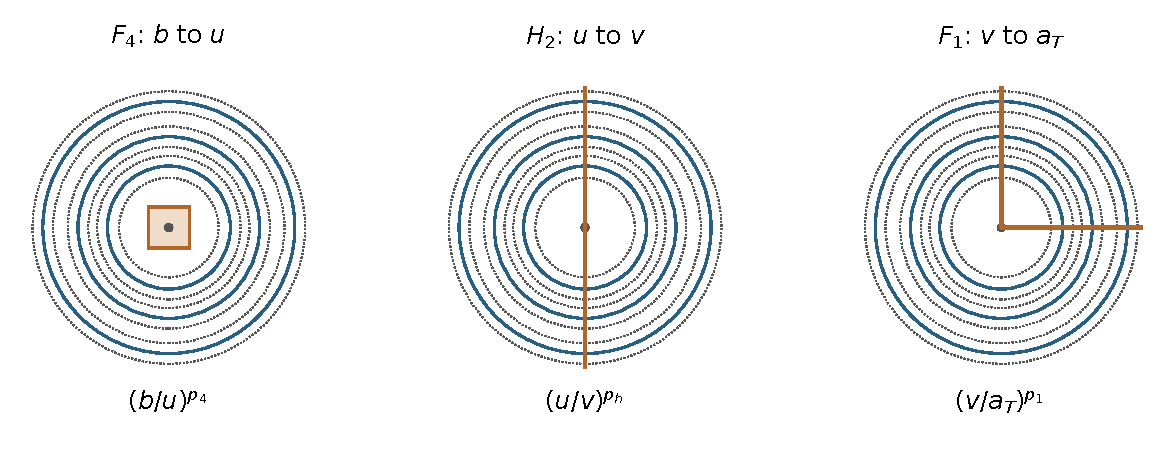
\includegraphics[width=\textwidth]{figures/pivotal-rings.pdf}
 \caption{The three ranges of checks forced by a pivotal square,
 schematically.  Blue rings have separated dotted collars; their centers
 may change between ranges.  Orange denotes the edit square, a side,
 and a vertex of the test, respectively, rather than a domain boundary.
 The drawing suppresses the actual contour passages and does not depict
 the literal gap ratios.  Enlarged environment neighborhoods fit in
 these separated collars, and the first retained ring avoids the
 environment stencil of the inserted mark.}
 \label{cross:fig-rings}
\end{figure}

\subsection{Conditional specifications and one reversal}

In the remainder of the proof lengths are lattice lengths unless a
factor $\delta$ is displayed.  Write $\eta$ for the full environment,
including the independent priorities and thresholds used to construct
the potentials.  A Gibbs variable includes both spins and reference
auxiliary variables, and is denoted by $\chi$.  At level $k$, in a finite
free chart $W$, with exterior configuration $\zeta$, the specification is
\begin{equation}
 \mu_{k,\eta,W}^{\zeta}(\dd\chi_W)
 =\frac{\exp F_{k,W}^{\zeta}(\chi_W)}
 {\mu_{0,W}^{\zeta}(\exp F_{k,W}^{\zeta})}
 \mu_{0,W}^{\zeta}(\dd\chi_W),\qquad
 F_{k,W}^{\zeta}=\sum_{j:\,\supp f_j^{(k)}\cap W\ne\varnothing}
 f_j^{(k)}(\chi_W\zeta_{W^c}).
 \label{cross:specification}
\end{equation}
The reference specification is pure critical Ising times its independent
reference auxiliary variables.  We may condition again in a smaller
free chart.  All suprema below include every exterior spin and auxiliary
assignment, so they also bound conditional laws with a random exterior.

Corollary~\ref{map:locality} allows the local construction to be performed
inside a free chart.  The prescribed exterior $\zeta$ contains only
level-$k$ field variables.  If a parent's complete decoration and
allocation stencil leaves $W$, set its $F_j$ to zero in every new coin
likelihood and retain its child logs.  Keep the full comparison stars
and the usual dummy coins.  Every fresh coin with a nontrivial
decoration is then sampled inside $W$.  Perform integrations only when
their full stencils lie in $W$.  Frozen terms, including terms entering
from outside $W$, are included in any
integration they meet; the exclusion rule still prevents a term from
meeting two integration squares.  Skip special integrations near the
boundary by the same rule.  The resulting identity is exact, and its
conditional specification agrees with the full level-$(k+1)$
specification at distance at least $C_1s_{k+1}$ from the boundary.
Only after constructing this joint output law do we condition outside
the eroded interior, whose exterior may now include fresh coins.
Disintegration gives a mixture of level-$(k+1)$ conditional
specifications; each is bounded by the corresponding exterior supremum.  This argument uses local conditional
identities, and does not condition on a favorable boundary event.

For a check on $A(z,\alpha;r,ar)$ take the surrounding chart
$W=S_{2ar}(z,\alpha)\setminus S_{r/2}(z,\alpha)$.  To iterate the
local construction in this fixed chart, allow the
available chart at level $k$ to be
$W_k=W\ominus M_1s_k$, where $\ominus t$ removes points within distance
$t$ of its boundary.  Choose $M_1$ so that
$M_1s_{k+1}\geq M_1s_k+C_1s_{k+1}$; it may also absorb allocated-support
overhangs.  Choose $M_0$ much larger than $M_1$ and all stencil constants.
Then a check with inner radius $r\geq M_0s_k$ retains the smaller
proportional collars chosen above in $W_k$, and successive interior steps
retain them as long as the check is still in this range.  Raise the first
retained radius, if necessary, so that the already fixed
ring gaps separate all environment stencils as well as the free charts.
The factor $G$ and the slack in \eqref{cross:slack} remain fixed.

By Proposition~\ref{map:reversal}, reversing step $k$ can change spins only in
squares of radius
\begin{equation}
 b_k=5s_{k+1},\qquad
 \E p_{x,k}(\eta)\leq C_LX_k,
 \label{cross:mark-bound}
\end{equation}
centered on the parent grid; increasing the fixed factor five absorbs
rounding if necessary.  Conditional on $\eta$, these Bernoulli marks
are mutually independent and independent of the entire new Gibbs
sample, including its fresh coins, before any further conditioning.
Their parameters depend only on environment variables within a fixed
multiple of $s_{k+1}$ of the center.  They can be placed at every candidate
center, independently of which integrations were selected.  The same
upper parameter envelope works for the localized construction.

For clarity, the elementary reason for this domination is a lower
likelihood-ratio bound.  If $S_x$ is a fixed constant times the sum of
child norms in the update stencil, then, conditional on the fresh coins
and the common exterior of the integration squares, the
before-integration law has density at least $e^{-S_x}$ relative to the
after-integration law.  It is therefore a
mixture with weight $e^{-S_x}$ of the new law and a residual probability
law.  On a Bernoulli mark of parameter $1-e^{-S_x}$ use the residual law;
otherwise retain the new sample.  Uniformly in all boundary data,
$1-e^{-S_x}\leq\min\{1,S_x\}$, which gives
\eqref{cross:mark-bound}.  Conditional separation of the update squares
permits independent marks, including for the special ratio integrations.
Integrating the discarded fresh coins out of the reconstructed decorated
law recovers the old spin law with its originally prescribed
level-$k$ exterior.

Given a spin configuration $\sigma$ and marks $M$ from just one reversal,
let $\mathcal C(\sigma,M)$ be the configurations agreeing with $\sigma$
off the marked squares.  For a Boolean test $T$, put
\begin{equation}
 \begin{aligned}
 T^+(\sigma,M)&=\1\{T(\widetilde\sigma)=1
       \text{ for some }\widetilde\sigma\in\mathcal C(\sigma,M)\},\\
 D_T(\sigma,M)&=\1\{T\text{ is not constant on }\mathcal C(\sigma,M)\}.
 \end{aligned}
 \label{cross:possibility}
\end{equation}
Both are increasing in the marks, irrespective of spin monotonicity.
For a check $T$ of inner radius $r$ in its prescribed annular chart, define
\begin{align}
 B_{k,T}(\eta)&=\sup_\zeta\mu_{k,\eta,W_k}^{\zeta}(T),\nonumber\\
 B^+_{k,T}(\eta)&=\sup_\zeta
  (\mu_{k,\eta,W_k}^{\zeta}\otimes\pi_{k-1,\eta})(T^+),
 \label{cross:envelopes}
\end{align}
where $\pi_{k-1,\eta}$ is the independent mark law for reversal of step
$k-1$.  At $k=0$ only the plain bound is used.  The supremum is taken
before environmental expectation.  Only finitely many exterior field
variables can enter these finite charts;
the auxiliary variables have finite alphabets, so these suprema are
measurable finite maxima.  Each quantity is a function only of
the environment in the chart and a fixed $O(s_k)$ neighborhood: these
are the supports of the potentials touching the chart and of the mark
parameters whose squares meet the test.  Mixtures over exterior data
need not have this locality; the suprema do.

\subsection{The product bound and the location count}

The next lemma supplies the single-step error.  Its hypothesis will be
proved by induction, first for the three fixed check shapes, and then
used for any prescribed polygonal test.

\begin{lemma}[A single-level pivotal bound]
\label{cross:single-level}
Let spins have the level-$k$ specification in a free chart, and allow
marks from step $k-1$, of radius $b=5s_k$.  Suppose the possibility envelope for every retained ring check satisfies
$\E B^+_{k,T_i}\leq q_i^0+\tau_i$.  The rings start at a sufficiently
large fixed multiple of $b$ and have disjoint collars enlarged by all
spin, mark, and environment stencils.  Then the expected conditional
supremum of the probability that a fixed test $T$ is changed by these
marks is at most
\begin{equation}
 C_TX_{k-1}\min\{1,(s_k/a_T)^c\},
 \label{cross:one-step-error}
\end{equation}
for a fixed $c>0$.  The same bound controls the increase from $T$ to
$T^+$.  Constants are uniform over translates, rotations, and dilates of
each of the three check shapes.  Any deterministic partial activation
of the marks satisfies the same estimates.
\end{lemma}

\begin{proof}
Activate the finitely many relevant marks in deterministic order.
For fixed $\eta$ and exterior data, conditioning on all previous marks
charges the first instability at $x$ to
$p_{x,k-1}(\eta)$ times a pivotal possibility event with that mark omitted.
If adding its square first permits two test values, choose a witnessing
assignment and revert the new square, retaining all the other assigned
values.  The resulting pair differs only in that square.  Every passage
required outside it by the geometric implication is consequently
possible using only the previous marks.  We may enlarge these to all
other marks in their respective ring neighborhoods.

Consider a retained family of rings with checks $T_1,\ldots,T_m$.
For fixed environment, condition off the first ring's eroded chart
$W_{1,k}$ and on the marks whose squares do not meet its spin support.  The other ring
checks are measurable under this conditioning; the remaining spins have
the specified conditional Gibbs law, and the remaining marks retain
their independent law.  Its factor is at most
$B^+_{k,T_1}(\eta)$.  Remove each ring in turn.  Pointwise in the original
exterior data this proves
\begin{equation}
 \sup_\zeta\bigl[p_{x,k-1}(\eta)
     \Prob_{k,\eta}^{\zeta}(T_1^+\cap\cdots\cap T_m^+)\bigr]
 \leq p_{x,k-1}(\eta)\prod_{\ell=1}^m B^+_{k,T_\ell}(\eta).
 \label{cross:quenched-product}
\end{equation}
The enlarged ring neighborhoods are disjoint and avoid the environment
stencil of $p_{x,k-1}$.  All factors on the right are therefore functions
of disjoint sets of the underlying independent environment variables.
Taking their expectation, including that of the inserted mark, gives
\begin{equation}
 \E\left[p_{x,k-1}\prod_{\ell=1}^m B^+_{k,T_\ell}\right]
 =\E p_{x,k-1}\prod_{\ell=1}^m\E B^+_{k,T_\ell}
 \leq C_LX_{k-1}\prod_{\ell=1}^m(q_{i(\ell)}^0+\tau_{i(\ell)}).
 \label{cross:annealed-product}
\end{equation}
This is why conditional exterior suprema, and the omission of rings
near the inserted square, are needed.  A product of unconditional
quenched check probabilities would not justify this equality.

Retain rings of ratio $a$ with successive inner radii in ratio $Ga$ in
each of the three ranges in \eqref{cross:distances}, illustrated in
Figure~\ref{cross:fig-rings}.  A fixed number of
omissions handles their endpoints, recenterings, and transitions.  By
\eqref{cross:slack}, the product in
\eqref{cross:annealed-product}, apart from $C_LX_{k-1}$, is at most
\begin{equation}
 C_T(b/u)^{p_4}(u/v)^{p_h}(v/a_T)^{p_1}.
 \label{cross:pivotal-power}
\end{equation}
If a range has too few scales for a retained ring, its bounded factor
loss is included in $C_T$.

It remains to sum over edit locations.  Normalize $a_T=1$ and suppose
$b<1$.  The centers with dyadically specified truncated distances $u,v$
occupy area at most $C_Tuv$: near a vertex, the portion of side at
distance $O(v)$ has length $O_T(v)$ and its $u$-neighborhood has that
area; away from vertices use the finite total side length.  The class
$u=v=1$ covers the remaining interior centers.  Since the center grid
has spacing comparable to $b$, enlarging each class by one grid cell
gives at most $C_Tuv/b^2$ centers.  Its contribution is bounded by
\begin{align}
 C_TX_{k-1}\frac{uv}{b^2}(b/u)^{p_4}(u/v)^{p_h}v^{p_1}
 &=C_TX_{k-1}(b/u)^{p_4-2}(u/v)^{p_h-1}v^{p_1}.
 \label{cross:area-sum}
\end{align}
Put $d=\min\{p_4-2,p_h-1,p_1\}>0$.
The three base ratios in the last expression have product $b$;
each dyadic class therefore contributes at most $C_TX_{k-1}b^d$.
There are $O_T((1+\log(1/b))^2)$ classes.  Absorb this factor into
$b^{d/2}$ and take $c=d/2$.  For $b\geq1$, only $O_T(1)$ grid centers
have squares meeting the test support, and the crude pivotal bound one
gives $C_TX_{k-1}$.  This proves \eqref{cross:one-step-error}, after
restoring $a_T$.  Finally $T^+-T\leq D_T$, and partial activation only
reduces the permitted mark parameters.
\end{proof}

\subsection{A bootstrap with geometrically weighted errors}

\begin{proposition}[Uniform conditional check bounds]
\label{cross:bootstrap}
Fix the preceding geometry and step constants.  There is $\varepsilon_*>0$
such that if the tuned trajectory satisfies $\sup_jX_j\leq\varepsilon_*$,
then, for every check $T_i$ of ratio $a$ and inner radius $r\geq M_0s_k$,
\begin{align}
 \E B_{k,T_i}
 &\leq q_i^0+C_{\rm boot}\sum_{j=k}^{J(r)}X_j(s_j/r)^c,
 \label{cross:plain-bootstrap}\\
 \E B^+_{k,T_i}
 &\leq q_i^0+C_{\rm boot}\sum_{j=k}^{J(r)}X_j(s_j/r)^c
          +C_{\rm boot}X_{k-1}(s_k/r)^c\qquad(k\geq1),
 \label{cross:possible-bootstrap}
\end{align}
where $J(r)=\max\{j:M_0s_j\leq r\}$.  Both right sides are at most
$q_i^0+\tau_i$.  The bounds hold uniformly over exterior data, frames,
and bulk torus charts, with the suprema interpreted as in
\eqref{cross:envelopes}.
\end{proposition}

\begin{proof}
We prove both assertions by strong induction on dyadic ranges of
$r/s_k$.  This induction includes all levels and all frames at once.
At a terminal ratio, $M_0s_k\leq r<M_0s_{k+1}$, only a bounded number
of level-$k$ potentials meet the free annular chart.  Put $S$ equal to
the sum of their norms.  Formula~\eqref{cross:specification} implies,
for every exterior assignment,
\[
 \|\mu_{k,\eta,W_k}^{\zeta}-\mu_{0,W_k}^{\zeta}\|_{\TV}
 \leq \min\{1,2S\},\qquad \E S\leq C_{\rm boot}X_k.
\]
Together with the pure bound $q_i^0$ this proves the terminal plain
estimate.  Since $s_k/r\geq(M_0L)^{-1}$, increasing the fixed constant
puts it in the form \eqref{cross:plain-bootstrap}.

For a nonterminal plain check, perform one step in its free chart.
Conditional on the remaining exterior, the new interior has its
level-$(k+1)$ specification.  Reversal and
\eqref{cross:possibility} bound its old probability by the new plain
probability plus the probability of instability under marks from step
$k$.  The new plain check has ratio $r/s_{k+1}=(r/s_k)/L$ and is already
covered by induction.  Every ring used to bound the instability has
inner radius at most $r/2$ and is evaluated at level $k+1$, with the
single-level possibility law there.  Its ratio to the level spacing is
strictly smaller than $r/s_k$, and it is monitored because the first
retained radius was chosen above a sufficiently large multiple of
$s_{k+1}$.  Its eroded collars remain in the region where the new
specification is valid.  Thus the inductive possibility bound supplies
the hypothesis of Lemma~\ref{cross:single-level}.  That lemma costs
$C X_k(s_{k+1}/r)^c$, which is a fixed multiple of
$X_k(s_k/r)^c$.  Adding it to the inductive plain estimate gives
\eqref{cross:plain-bootstrap}.

Once the plain estimate at a given ratio has been proved, bound its
possibility increase using marks from step $k-1$.  Its pivotal rings
are now at level $k$, with inner radii at most $r/2$, so their
possibility bounds belong to strictly smaller dyadic ranges of $r/s_k$.
Lemma~\ref{cross:single-level} gives the last term in
\eqref{cross:possible-bootstrap}.  This also proves the terminal
possibility estimate.  If no monitored ring fits between the required
first radius and the cutoff, the test size and edit radius differ by a
bounded factor; the crude bounded count of candidate marks gives the
same estimate without a recursive call.  This starts the induction.

To close it, the geometric spacing gives
\[
 \sum_{j=k}^{J(r)}(s_j/r)^c
 \leq \frac{M_0^{-c}}{1-L^{-c}}.
\]
Choose $C_{\rm boot}$ to cover the terminal comparison and the two
one-level additions, and then choose $\varepsilon_*$ so that this
weighted sum and the additional single-level term are smaller than
$\min_i\tau_i$.  In each inductive call only these fixed tolerances
were used to obtain the pivotal power.  This proves both estimates
without any assumption about a configuration edited at several levels.
\end{proof}

We have obtained the passage bounds needed for a test of any fixed
geometry.  Its geometry changes $C_T$ and $a_T$, but never the smallness
threshold: Lemma~\ref{cross:single-level} can now use
Proposition~\ref{cross:bootstrap} on every retained ring.

\subsection{Macroscopic and local comparisons}

The elementary limit underlying all the remaining comparisons is
\begin{equation}
 \sum_{j=0}^{K-1}X_j\min\{1,(\delta s_{j+1}/a_*)^c\}\longrightarrow0
 \quad\text{if }X_j\to0,\quad K\to\infty,
 \quad\sup_K\delta s_K<\infty,
 \label{cross:weighted-vanishing}
\end{equation}
for every fixed $a_*>0$.  Indeed, for $j\geq m$, replace $X_j$ by
$\sup_{j\geq m}X_j$.  The remaining geometric weights have a uniformly
bounded sum, because $s_{j+1}/s_K=L^{j+1-K}$; the finitely many indices
$j<m$ tend to zero separately.  Send $m\to\infty$ afterwards.  Thus
\eqref{cross:weighted-vanishing} uses decay of $X_j$, not its summability.

\begin{proposition}[Quenched torus test comparison]
\label{cross:torus-comparison}
Fix a finite family $\mathcal T$ of polygonal corridor crossings, band
circuits, and the three annular passage checks, in a common buffered
planar chart.
Take tori of period $Ms_K$, where $M$ is a sufficiently large fixed
integer, $K\to\infty$, and their physical periods $\delta Ms_K$ stay in
a fixed compact interval large enough to contain this chart.  If
$\nu_{0,\omega}^{\mathcal T}$ and $\nu_{\rm pure}^{\mathcal T}$ are the
quenched level-zero and pure laws of the whole test vector, then
\begin{equation}
 \E_{\rm env}\|\nu_{0,\omega}^{\mathcal T}
                    -\nu_{\rm pure}^{\mathcal T}\|_{\TV}\longrightarrow0.
 \label{cross:torus-tv}
\end{equation}
Such periods can be chosen for every sequence $\delta\downarrow0$.
\end{proposition}

\begin{proof}
Couple each successive level by the reversal in
Proposition~\ref{map:reversal}.  After averaging over the environment,
the probability that a test changes at step $j$ is at most
\[
 C_TX_j\min\{1,(\delta s_{j+1}/a_T^{\rm phys})^c\}.
\]
This follows from Lemma~\ref{cross:single-level} and
Proposition~\ref{cross:bootstrap}; if the test is no larger than the
edit square, use the crude candidate count.  Sum over steps and the
fixed family.  Equation~\eqref{cross:weighted-vanishing} makes the sum
vanish.  At level $K$ only a bounded number of potentials remain on
the torus, so their expected total norm is $O_M(X_K)$.  The same density
comparison as in the terminal bootstrap couples this level to the pure
torus with expected total variation tending to zero.  Gluing the
successive couplings and using the union bound proves
\eqref{cross:torus-tv}.  Only the errors of individual reversals were
summed; no probability estimate was imposed on the union of their marks.

The level-zero quenched probabilities depend only on the original bond
environment $\omega$.  Averaging the bounds over the auxiliary algorithm
choices therefore leaves exactly the expectation in
\eqref{cross:torus-tv}.  Finally, choosing $K$ by the first scale above
a fixed multiple of $\delta^{-1}$ keeps the physical period between two
fixed bounds whose ratio is $L$.
\end{proof}

\begin{proposition}[Uniform local conditional comparison]
\label{cross:local-comparison}
Fix a bounded polygonal geometry with a finite family $\mathcal T$ of
corridor crossings, band circuits, or the three annular passage checks
strictly inside its free buffers; annular windows may have both
an inner and an outer free collar.  Dilate this geometry by $r$ in
lattice units, where $r\to\infty$.  There is a nonnegative envelope
$\mathcal E_r(\eta)$, independent of exterior Gibbs data, such that
$\E\mathcal E_r\to0$, uniformly in the translated center and the position
of the scale grids.  For every exterior assignment the quenched joint
test law is within $\mathcal E_r(\eta)$ in total variation of a mixture
of pure conditional test laws on a still-buffered interior window.
Consequently every positive pure lower bound uniform over those
conditional laws transfers with any strictly smaller bound, outside
an environment event whose probability tends to zero.
\end{proposition}

\begin{proof}
Choose the terminal spacing $s_K$ comparable to $r$ with a sufficiently
small fixed proportionality constant depending on this geometry.
Run the local construction through level $K$.  The sum of the removed
boundary thicknesses is $O(s_K)$, so this choice leaves all prescribed
buffers free.  At each reversal use the conditional-supremum version
of \eqref{cross:quenched-product}.  For example, a measurable upper
bound for the error is the sum over inserted centers of their mark
parameters times the products of local ring suprema, with the factor
one when only the crude count is used.  These functions depend on
local environment, and bound the error for every exterior assignment
before any mixture of those assignments is taken.  Summing them over
steps and the finite family gives an envelope with expectation at most
\[
 C_{\mathcal T}\sum_{j=0}^{K-1}X_j
       \min\{1,(s_{j+1}/r)^c\}.
\]
At the terminal scale add
$C\min\{1,\sum_j\|f_j^{(K)}\|\}$ over potentials touching the remaining
window.  Their number is bounded, so this contribution has expectation
$O_{\mathcal T}(X_K)$.  Conditional on its exterior, deleting those
potentials gives the pure conditional law; integrating the exterior
produces the stated mixture.  Formula~\eqref{cross:weighted-vanishing},
with effective mesh $r^{-1}$, proves the vanishing expectation.

If every pure conditional law gives an event probability at least
$c_*>0$, the perturbed probability is at least
$c_*-\mathcal E_r(\eta)$ for every initial exterior.  Markov's inequality
then transfers any lower bound less than $c_*$.  In particular this
applies to the fixed compatible systems of buffered colored corridors
and circuits in \cite[Section~2, Proposition ``Pure buffered RSW
consequences'']{S}.  To state the result using only the original bond
environment, average the envelope over the algorithm choices.  The
worst level-zero conditional probability itself depends only on the
bonds in the window and its incident layer; hence its good-environment
event is local.  All estimates are uniform in the center, whereas their
convergence rate may depend on the fixed geometry.
\end{proof}

\begin{corollary}[No interior four-passage bottlenecks]
\label{cross:four-passages}
Let a compact set $K_0$ have fixed positive clearance from the boundary
of a finite domain, and fix a sufficiently small physical radius $R>0$.
At the tuned couplings, uniformly in boundary spin assignments,
\begin{equation}
 \lim_{r\downarrow0}\limsup_{\delta\downarrow0}
 \E_{\rm env}\mu_\omega\bigl(
   \text{some }z\in K_0\text{ has four passages from }r\text{ to }R
                              \bigr)=0.
 \label{cross:four-passages-limit}
\end{equation}
Passages are counted with the parameter-interval convention above.
\end{corollary}

\begin{proof}
For a specified center, pack separated rings of ratio $a$ from a fixed
multiple of $r$ to a fixed fraction of $R$.  At every fixed physical
$r>0$, their inner lattice radii eventually exceed $M_0s_0$.
Condition off their free charts as in \eqref{cross:quenched-product}
and use the plain bound of Proposition~\ref{cross:bootstrap}.
Their environment neighborhoods are disjoint, so
\eqref{cross:annealed-product}, without an inserted mark, yields
\[
 \E_{\rm env}\mu_\omega(F_4(z;r,R))\leq C(r/R)^{p_4}
\]
in the mesh upper limit, with $p_4>2$.  The bound already includes the
supremum over exterior data of the ambient domain.  For fixed $r$,
cover $K_0$ by an $r$-grid of $O_{K_0}(r^{-2})$ centers.  Enlarge the
inner squares and reduce the outer radius by fixed factors, so four
passages about any center imply a grid check.  A union bound gives
$C_{K_0,R}r^{p_4-2}$ after the mesh limit, which tends to zero.  The
finite test family is enlarged only after its mesh limit has been taken;
lattice rounding is absorbed by the same fixed crops.
\end{proof}

All smallness conditions in this section involve the three check shapes
and fixed flow parameters.  They can therefore be imposed by shrinking
one weak-randomness interval before any final domain or test geometry
is chosen.  The local comparison supplies FK barriers for the
identification of the physical threshold.  The torus comparison supplies
the signed boundary barriers used to identify the limiting interface,
and the passage exclusion controls its backtracking.

\section{Identification of the physical critical point}
\label{sec:criticality}

The parameter furnished by Theorem~\ref{traj:critical-trajectory} was
chosen by its scale evolution. We first identify that parameter by torus
duality, and then show that it is the threshold for plus magnetization.
The second step uses the uniform local comparison from
Proposition~\ref{cross:local-comparison}; self-duality alone will not be
used as a criterion for criticality.

Fix a sufficiently small $\theta>0$. Throughout this section the bond
couplings and their FK odds are
\begin{equation}
 v_e(h,\omega):=e^{2K_e(h,\omega)}-1
       =\sqrt2\,e^{h+\theta\xi_e(\omega)},
 \qquad h\in\R.
 \label{crit:odds}
\end{equation}
The original signs $\xi_e$ are independent and symmetric. Auxiliary
random choices used in the scale construction are integrated out whenever
we discuss the original spin or FK law.

For a finite graph $G=(V,E)$ and a partition $\pi$ of its boundary
vertices, write $\phi_{G,h,\omega}^{\pi}$ for the random-cluster measure
\begin{equation}
 \phi_{G,h,\omega}^{\pi}(\eta)
 =\frac{1}{\mathcal Z_{G,h,\omega}^{\pi}}
       2^{k_\pi(\eta)}\prod_{e\in E}v_e(h,\omega)^{\eta_e},
 \qquad \eta\in\{0,1\}^{E}.
 \label{crit:fk}
\end{equation}
Here $k_\pi(\eta)$ counts open clusters after identifying the vertices
in each part of $\pi$. The superscript $\mathrm w$ means that all boundary
vertices are identified. Unless explicitly stated otherwise, a path uses
ordinary lattice edges and does not use these identifications. At fixed
environment the measures in \eqref{crit:fk} are monotonic, satisfy FKG,
and increase with each edge odds and with boundary wiring. These are the
usual finite-volume FK properties; their Edwards--Sokal coupling to the
Ising model is given in~\cite{ES}.
We write $\phi_{h,\omega}^{\mathrm w}$ for the infinite-volume wired
measure, obtained by the monotone limits of finite wired boxes.

We use the following form of the decision-tree inequality. If $A$ is an
increasing event and a decision tree determines $A$ under a finite
monotonic measure $\phi$, then
\begin{equation}
 \phi(A)\bigl(1-\phi(A)\bigr)
 \le \sum_{e\in E}\delta_e\,
       \operatorname{Cov}_{\phi}(\1_A,\eta_e),
 \label{crit:osss}
\end{equation}
where $\delta_e$ is the probability that the tree queries $e$
\cite[Theorem~1.1]{DCRT}. The inequality also holds after averaging over
an independent choice of tree. For \eqref{crit:fk}, differentiation at
fixed environment gives the exact identity
\begin{equation}
 \frac{\dd}{\dd h}\phi_{G,h,\omega}^{\pi}(A)
 =\sum_{e\in E}
       \operatorname{Cov}_{\phi_{G,h,\omega}^{\pi}}(\1_A,\eta_e).
 \label{crit:derivative}
\end{equation}
Indeed, varying $h$ multiplies the unnormalized weight by
$\exp(h\sum_e\eta_e)$, apart from its $h$-independent factors. Both
\eqref{crit:osss} and \eqref{crit:derivative} will be applied before
averaging over environments.

\subsection{Torus duality fixes the tuned parameter}

Let $\mathbb T_N=(\Z/N\Z)^2$, with $N\ge3$. A spin holonomy
$\alpha=(\alpha_1,\alpha_2)\in\{0,1\}^2$ prescribes the signs acquired
by a spin after one turn around the two coordinate cycles. Equivalently,
choose edge signs $\tau_e^\alpha$ whose product around every elementary
face is $1$ and whose products around the two coordinate cycles are
$(-1)^{\alpha_1}$ and $(-1)^{\alpha_2}$. Define
\[
 Z_\alpha(K)=\sum_{\sigma\in\{-1,1\}^{\mathbb T_N}}
       \exp\left(\sum_{e=\{x,y\}}K_e\tau_e^\alpha\sigma_x\sigma_y\right).
\]
Changing the representative $\tau^\alpha$ by a vertex gauge
transformation does not change this sum. Write $Z(K)$ for the vector of
these four partition functions, ordered as $00,10,01,11$, and put
$\widehat Z(K)=Z(K)/\|Z(K)\|_2$.

\begin{lemma}[The four torus partition functions]
\label{crit:torus-identities}
For positive couplings on $\mathbb T_N$, $N\ge3$, let the dual couplings satisfy
$e^{-2K_{e^*}^*}=\tanh K_e$. Identify the dual square torus with the
original one by a half-lattice translation. Then
\begin{equation}
 Z(K)=a(K)\mathsf H Z(K^*),\qquad
 a(K)=\prod_e\sqrt{\sinh(2K_e)},\qquad
 \mathsf H=\frac12
 \begin{pmatrix}
 1&1&1&1\\
 1&1&-1&-1\\
 1&-1&1&-1\\
 1&-1&-1&1
 \end{pmatrix}.
 \label{crit:torus-duality}
\end{equation}
In particular $\mathsf H$ is orthogonal and fixes the pure critical
vector. For every holonomy $\alpha$,
\begin{equation}
 \frac{Z_\alpha(K)}{Z_{00}(K)}
 =\phi_{\mathbb T_N,K}
 \left(\alpha([\gamma])=0
       \text{ for every open cycle }\gamma\right),
 \label{crit:torus-ratio}
\end{equation}
where $[\gamma]\in(\Z/2\Z)^2$ is the cycle's winding class and
$\phi_{\mathbb T_N,K}$ is the untwisted torus FK law.
\end{lemma}

\begin{proof}
We record the finite-volume form of Kramers--Wannier duality
\cite{KW}, including its homology convention; the four-sector matrix
also appears in \cite[Equations~(4)--(5)]{BS}. For
$b\in(\Z/2\Z)^2$, let
\[
 W_b(K)=\sum_{\substack{A\subset E(\mathbb T_N)\text{ even}\\{}[A]=b}}
                    \prod_{e\in A}\tanh K_e.
\]
The high-temperature expansion gives
\[
 Z_\alpha(K)=2^{N^2}\prod_e\cosh K_e
                  \sum_b(-1)^{\alpha\cdot b}W_b(K).
\]
The low-temperature expansion of the dual spin system with holonomy
$\beta$ has domain walls of winding class
$(\beta_2,\beta_1)$. Each admissible wall configuration comes from two
spin configurations, so
\[
 Z_\beta(K^*)=2e^{\sum_eK_{e^*}^*}
                   W_{(\beta_2,\beta_1)}(K).
\]
Substitution gives the sign
$(-1)^{\alpha_1\beta_2+\alpha_2\beta_1}$ in
\eqref{crit:torus-duality}. Its prefactor follows from
$|E(\mathbb T_N)|=2N^2$ and
$e^{-K_{e^*}^*}\cosh K_e=\sqrt{\sinh(2K_e)/2}$.
At $K_e=K_0$, the dual couplings equal $K_0$ and $a(K)=1$; hence
$\mathsf HZ(K_0)=Z(K_0)$. The displayed matrix satisfies
$\mathsf H^2=I$.

For the ratio, expand each edge factor as
\[
 e^{K_e\tau_e^\alpha\sigma_x\sigma_y}
 =e^{-K_e}\left(1+v_e\,
           \1_{\{\sigma_x=\tau_e^\alpha\sigma_y\}}\right).
\]
On a chosen open subgraph the spin constraints are consistent exactly
when every open cycle has zero evaluation under $\alpha$. In that case
there are $2^{k(A)}$ compatible spin assignments. Dividing the resulting
sum by its untwisted version proves \eqref{crit:torus-ratio}.
\end{proof}

\begin{proposition}[Identification of the tuned parameter]
\label{crit:self-dual-tuning}
The value $h_*$ furnished by
Theorem~\ref{traj:critical-trajectory} is zero.
\end{proposition}

\begin{proof}
Choose a fixed large integer $M$ and torus periods $N_k=Ms_k$, so that
every complete support and environment-dependence neighborhood of
Proposition~\ref{map:step}, through scale $k$, embeds in the torus.
The primitive environment variables in each such neighborhood have
their plane distribution, so each resulting potential has its plane
law when expressed in local spin coordinates. Apply the
scale construction with iid torus disorder, simultaneously in the four
spin holonomies. Let $\zeta$ denote the independent algorithmic choices
used in this run. In every contractible neighborhood a flat twist has a
spin trivialization; changes of trivialization on overlaps are constant
spin flips. Every interaction is even, and the auxiliary variables are
unchanged by spin flip. The local identities therefore hold in each
holonomy, with the same scalar factors removed by centering. In
particular, for a common positive factor $c_k(\omega,\zeta)$ the resulting
partition functions satisfy
\[
 e^{-S_k}Z_\alpha(K_0)
 \le c_k(\omega,\zeta)^{-1}Z_\alpha(K(h_*,\omega))
 \le e^{S_k}Z_\alpha(K_0),
\]
where $S_k=S_k(\omega,\zeta)$ can be the largest, over the four holonomies, of the sums of
norms of the remaining potentials. There are only $M^2$ cells at the
last scale. The trajectory bound $X_k\to0$ gives
$\E S_k\le C M^2 X_k\to0$. Consequently
\begin{equation}
 \bigl\|\widehat Z(K(h_*,\omega))-
                 \widehat Z(K_0)\bigr\|_2\longrightarrow0
 \quad\text{in environmental probability}.
 \label{crit:torus-terminal}
\end{equation}
The partition vector itself does not depend on the algorithmic choices,
so this conclusion also holds after retaining only the original bond
environment.

The dual odds satisfy $v_{e^*}^*=2/v_e$. Thus duality sends
$(h,\xi_e)$ to $(-h,-\xi_e)$, with the signs transported along the
crossing-edge bijection. This transformation preserves their iid law.
By Lemma~\ref{crit:torus-identities}, the normalized duality transform is
the orthogonal matrix $\mathsf H$, and its pure target is fixed.
Therefore \eqref{crit:torus-terminal} holds with $-h_*$ as well.

Take $\alpha=10$, and let $A_\alpha$ be the increasing event that some
open cycle has odd evaluation under $\alpha$. Its pure probability
$q_N^0$ satisfies
\begin{equation}
 c\le q_N^0\le1-c
 \label{crit:pure-torus-nondegeneracy}
\end{equation}
uniformly for large $N$. For the lower bound, a finite chain of pure FK
rectangle crossings in a torus band constructs an open cycle winding
once horizontally. For the upper bound, the corresponding construction
of a closed-dual cycle winding once vertically prevents such an open
cycle. The constructions use finitely many embedded rectangles of fixed
aspect ratios and the uniform pure FK bounds recalled in
\cite[Section~2, ``Pure buffered RSW consequences'']{S}.
They can be imposed successively with arbitrary induced boundary wiring;
for a closed-dual crossing use the worst, fully wired primal boundary.

All ratios in \eqref{crit:torus-ratio} belong to $[0,1]$, so the
untwisted coordinate of $\widehat Z$ is at least $1/2$. Hence
\eqref{crit:torus-terminal} implies, on the same original signs,
\[
 q_{N_k,\omega}(h_*)-q_{N_k}^0\longrightarrow0,
 \qquad
 q_{N_k,\omega}(-h_*)-q_{N_k}^0\longrightarrow0
\]
in probability, where $q_{N,\omega}(h)=
\phi_{\mathbb T_N,h,\omega}(A_\alpha)$. The two convergence statements
hold simultaneously by a union bound. Querying every edge in
\eqref{crit:osss} and using \eqref{crit:derivative} gives
$q'_{N,\omega}(h)\ge q_{N,\omega}(h)(1-q_{N,\omega}(h))$.
If $h_*\ne0$, monotonicity and
\eqref{crit:pure-torus-nondegeneracy} keep this product bounded below on
the interval between $-h_*$ and $h_*$, with probability tending to one.
Integration forces an endpoint difference bounded below by a positive
constant, whereas both endpoints approach the same $q_{N_k}^0$.
This contradiction proves $h_*=0$.
\end{proof}

\subsection{From local barriers to sharpness}

We now use the local crossing comparison at $h=0$. Put
$B_r(x)=\{y\in\Z^2:|y-x|_\infty\le r\}$ and $B_r=B_r(0)$.
All annuli below have deterministic lattice boundaries; changing them by
a bounded incident layer changes none of the estimates.

\begin{lemma}[Local FK barriers]
\label{crit:ring-barrier}
There are fixed $a>1$ and $c_0>0$ with the following property. Let
$\mathcal A(x,r)$ be the lattice annulus
$B_{ar}(x)\setminus B_r(x)$, and let $\mathcal R(x,r)$ be its ordinary
radial crossing event. Call its bond environment good if
\[
 \phi_{\mathcal A(x,r),0,\omega}^{\mathrm w}
       (\mathcal R(x,r))\le1-c_0,
\]
where both boundary components are wired together. The probability that the
environment is not good tends to zero as $r\to\infty$, uniformly in
$x$. Goodness is a function only of the bonds of that annulus and its
incident layer. Every good annulus has the same crossing upper bound
for all $h\le0$ and all less wired boundary conditions. In particular,
\begin{equation}
 \E\phi_{0,\omega}^{\mathrm w}(0\leftrightarrow\infty)=0.
 \label{crit:no-percolation-at-tuning}
\end{equation}
\end{lemma}

\begin{proof}
Choose two separated buffered subbands of an annulus of fixed sufficiently
large ratio $a$. The pure probability of simultaneous plus and minus spin
circuits, one in each subband, is bounded below by a constant $2c_0>0$,
uniformly over pins outside the buffers; this is precisely
\cite[Section~2, Proposition ``Pure buffered RSW consequences'']{S}.
Proposition~\ref{cross:local-comparison} transfers this lower bound to
the random spin law, with probability tending to one over the local
environment and uniformly over the boundary pins. Apply it to
Edwards--Sokal spins with the wired boundary cluster pinned plus.
An ordinary open FK path has a constant spin. Such a path cannot cross
both separating circuits of opposite colors. The common triangulation
used for spin circuits causes no exception: a nearest-neighbor lattice
path can cross a circuit only through a vertex of that circuit. The
ordinary radial FK crossing probability is thus at most $1-c_0$.

Defining goodness by this wired crossing probability makes it a function
of the original local bonds alone. Its failure probability tends to zero
after integrating out all algorithmic choices. FK monotonicity gives
the assertion for $h\le0$ and for weaker wiring.

For completeness, this also rules out percolation at $h=0$. Pack
concentric annuli with a fixed large geometric separation, so that their
bond sets, including incident layers, are disjoint. Conditional on all
edges off one annulus, its induced FK boundary partition is dominated by
full wiring. The probability of an arm crossing $m$ such annuli is
therefore bounded, at fixed environment, by the product of their fully
wired crossing bounds. Choose the first radius large enough that every
bad-annulus probability is at most $1/2$. Independence of the local bond
sets bounds the environmental mean of this product by
$(1-c_0/2)^m$. Letting $m\to\infty$ in the wired infinite-volume limit
proves \eqref{crit:no-percolation-at-tuning}.
\end{proof}

The preceding lemma gives no rate for the probability of a bad annulus.
The next proof obtains the rate needed for sharpness by using many
independent annuli, before applying the decision-tree inequality.

\begin{lemma}[Subcritical arms]
\label{crit:subcritical-arms}
For every $b>0$ and $A>0$ there is $C_{b,A}<\infty$ such that
\begin{equation}
 \E\phi_{B_{2N}(x),-b,\omega}^{\mathrm w}
 \bigl(x\leftrightarrow\partial B_N(x)
                \text{ inside }B_N(x)\bigr)
       \le C_{b,A}N^{-A}.
 \label{crit:annealed-arm}
\end{equation}
The same bound holds for the ordinary path event under any finite or
infinite-volume FK law whose domain contains $B_{2N}(x)$, with arbitrary
boundary condition outside that box.
\end{lemma}

\begin{proof}
We work at $x=0$; the estimates are uniform over translates. For every
vertex $z\in B_{N+1}$, pack $m_N\ge c\log N$ separated annuli centered
at $z$, with inner radii between $N^{1/4}$ and a sufficiently small
multiple of $N^{1/2}$. Their full annular graphs lie in
$B_{N^{1/2}}(z)$, and their bond neighborhoods are disjoint. Let
$\eta_N\to0$ be an upper bound for their bad-environment probabilities,
uniformly over all these radii and centers, provided by
Lemma~\ref{crit:ring-barrier}. Independence for the annuli around one
fixed $z$ gives
\[
 \Prob\bigl(\text{at least }m_N/2\text{ annuli at }z
                      \text{ are bad}\bigr)
       \le 2^{m_N}\eta_N^{m_N/2}.
\]
Let $\mathcal G_N$ be the event that fewer than half are bad at every
$z\in B_{N+1}$. A union bound, without any independence assertion
between distinct centers, gives
\begin{equation}
 \Prob(\mathcal G_N^c)
 \le C N^2 2^{m_N}\eta_N^{m_N/2}
       =o(N^{-A})\qquad\text{for every }A>0.
 \label{crit:environment-exception}
\end{equation}
Indeed $m_N$ is bounded above and below by constant multiples of
$\log N$, while $\log(1/\eta_N)\to\infty$.

On $\mathcal G_N$, multiplication of the good-annulus bounds gives,
for some fixed $\alpha>0$,
\begin{equation}
 \phi_{B_{2N},h,\omega}^{\mathrm w}
 \bigl(z\leftrightarrow\partial B_{N^{1/2}}(z)
                   \text{ inside }B_{N^{1/2}}(z)\bigr)
       \le C N^{-\alpha},
 \qquad z\in B_{N+1},\quad h\le0.
 \label{crit:uniform-short-arm}
\end{equation}
For large $N$ all these small boxes lie within $B_{2N}$. Induced
boundary conditions are harmless because the annular bounds already
use full wiring. The event $\mathcal G_N$ works simultaneously for
every $h\le0$ by monotonicity.

Fix such an environment and write
\[
 q_\omega(h)=\phi_{B_{2N},h,\omega}^{\mathrm w}
     (0\leftrightarrow\partial B_N\text{ inside }B_N).
\]
Choose an integer $\ell$ uniformly between $N/4$ and $N/2$, and
explore all ordinary open clusters in $B_N$ that meet the layer
$\partial B_\ell$. This determines the event defining $q_\omega$:
every path from $0$ to $\partial B_N$ meets that layer. The exploration
uses only ordinary edges in $B_N$, although its law is the marginal
of the wired measure on $B_{2N}$. This is the layer exploration of
\cite[Lemma~3.2 and its proof]{DCRT}.

An edge is queried only if an endpoint lies on the chosen layer or
has an ordinary open path to it. For a fixed endpoint $z$, the
probability, over $\ell$, that the layer is within distance
$N^{1/2}$ of $z$ is at most $C N^{-1/2}$. Otherwise such a path forces
an arm of length $N^{1/2}$ at $z$. Thus
\eqref{crit:uniform-short-arm} bounds the maximum averaged revealment
by
\[
 \max_e\delta_e\le C\bigl(N^{-1/2}+N^{-\alpha}\bigr)
                   \le C N^{-d},\qquad
 d=\min\{1/2,\alpha\}>0.
\]
Edges outside $B_N$ have revealment zero. Their covariances are
nonnegative, so retaining them in the derivative sum only strengthens
the bound obtained from \eqref{crit:osss}. Equations
\eqref{crit:osss}--\eqref{crit:derivative} yield, for all $h\le0$,
\begin{equation}
 q'_\omega(h)\ge cN^d q_\omega(h)(1-q_\omega(h)).
 \label{crit:sharp-differential}
\end{equation}
Moreover \eqref{crit:uniform-short-arm} at $z=0$ gives
$q_\omega(0)\le C N^{-\alpha}$. For sufficiently large $N$, integrating
the derivative of $\log(q_\omega/(1-q_\omega))$ over $[-b,0]$ gives
\[
 \frac{q_\omega(-b)}{1-q_\omega(-b)}
 \le \frac{q_\omega(0)}{1-q_\omega(0)}e^{-cbN^d}
 \le e^{-cbN^d}.
\]
Combining this estimate with \eqref{crit:environment-exception} proves
\eqref{crit:annealed-arm}. In a larger graph, condition outside
$B_{2N}(x)$ and dominate the induced boundary partition by full
wiring. This proves the final assertion, including infinite-volume
limits.
\end{proof}

\subsection{The magnetization threshold}

The preceding results now identify the physical temperature. Put
$m_\theta(h)=\E\phi_{h,\omega}^{\mathrm w}(0\leftrightarrow\infty)$.
Edwards--Sokal identifies this with the environmental mean of the
infinite-volume plus magnetization. Under the plus boundary convention of
Section~\ref{sec:introduction}, the finite FK graph contains all bonds meeting the spin box,
and all exterior endpoints are wired and assigned spin plus. Shifting
the wired boundary by one lattice layer sandwiches this law between
the usual wired-box laws, so their infinite-volume limits agree.

\begin{theorem}[Physical critical point]
\label{crit:physical}
For every sufficiently small fixed $\theta>0$,
\[
 m_\theta(h)=0\quad(h\le0),\qquad
 m_\theta(h)>0\quad(h>0).
\]
Consequently, for every sufficiently small $\epsilon>0$, the critical
inverse temperature in Theorem~\ref{thm:main} is the unique positive
solution of
\begin{equation}
 \bigl(e^{2\beta_c(\epsilon)(1+\epsilon)}-1\bigr)
 \bigl(e^{2\beta_c(\epsilon)(1-\epsilon)}-1\bigr)=2.
 \label{crit:physical-equation}
\end{equation}
The plus magnetization is zero at this temperature.
\end{theorem}

\begin{proof}
Lemma~\ref{crit:ring-barrier} and monotonicity give $m_\theta(h)=0$
for $h\le0$. Fix $h=b>0$. Planar FK duality replaces the edge odds
by $2/v_e$, so the dual environment has the law of the model at $-b$.
In finite domains the dual boundary condition is dominated by full
wiring. Taking limits, the dual of the infinite-volume wired primal
law therefore satisfies the local annealed arm bounds of
Lemma~\ref{crit:subcritical-arms}.

A closed-dual circuit surrounding $B_M$ whose farthest distance from
the origin lies in $[R,2R)$ has diameter at least $cR$. It consequently
contains an ordinary dual arm of length $c'R$ from some dual vertex
in $B_{2R}$, with absolute positive constants $c,c'$. There are
$O(R^2)$ possible vertices. Using \eqref{crit:annealed-arm} with any
$A>2$ and summing over dyadic $R\ge c''M$ gives
\begin{equation}
 \E\phi_{b,\omega}^{\mathrm w}
 \bigl(\text{a closed-dual circuit surrounds }B_M\bigr)
 \le C_{b,A}\sum_{j\ge0}(2^jM)^{2-A}
 \longrightarrow0.
 \label{crit:dual-circuits}
\end{equation}
Here the arm bound is applied in a box of radius comparable with
$R$, with a further collar of comparable width; its validity for
arbitrary exterior boundary conditions was part of
Lemma~\ref{crit:subcritical-arms}.

If every open cluster meeting $B_M$ were finite, their union would
be finite. It contains $B_M$, and its lattice edge boundary consists
of closed edges. Connecting the union through the box, if necessary,
does not change its exterior boundary. Its outer dual boundary
therefore contains a closed-dual circuit surrounding $B_M$.
The complement of the event in \eqref{crit:dual-circuits} thus forces
some vertex of $B_M$ to belong to an infinite open cluster. For large
$M$ this has positive joint probability. The joint environment--wired
FK law is translation invariant, whence
\[
 0<\E\phi_{b,\omega}^{\mathrm w}(B_M\leftrightarrow\infty)
 \le |B_M|\,m_\theta(b).
\]
This proves positivity for every $b>0$.

Finally, the left side of \eqref{crit:physical-equation}, viewed as
a function of $\beta\ge0$, is continuous and strictly increasing
from zero to infinity. Let $\beta_*$ be its unique solution, and set
\[
 v_\pm=e^{2\beta_*(1\pm\epsilon)}-1,
 \qquad
 \theta_\epsilon=\frac12\log\frac{v_+}{v_-}.
\]
Then $v_\pm=\sqrt2e^{\pm\theta_\epsilon}$. Comparison with the
constant couplings gives
$K_0/(1+\epsilon)\le\beta_*\le K_0/(1-\epsilon)$, so
$\theta_\epsilon\to0$ as $\epsilon\to0$. The model at $\beta_*$
therefore falls within the result just proved and has zero plus
magnetization. The same holds below $\beta_*$ by monotonicity.
For $\beta>\beta_*$ both log odds increase, and
\[
 b:=\min_{s\in\{-1,1\}}
       \log\frac{e^{2\beta(1+s\epsilon)}-1}
                    {e^{2\beta_*(1+s\epsilon)}-1}>0.
\]
The bonds at $\beta$ dominate those of
\eqref{crit:odds} with parameters $(b,\theta_\epsilon)$ in the
same sign environment. Their plus magnetization is consequently
positive. This proves $\beta_*=\beta_c(\epsilon)$ with the
normalization and plus boundary convention of Theorem~\ref{thm:main}.
\end{proof}

\section{From bulk comparisons to quenched curves}
\label{sec:curves}

We now work at the physical critical point identified in
Theorem~\ref{crit:physical}.  The bulk comparisons of
Section~\ref{sec:crossings} will yield couplings between the target
interface and pure interfaces in slightly displaced domains.  The pure
marginal in each coupling will remain fixed after conditioning on the
environment.  This conditional marginal property is what turns the
geometric argument into convergence of quenched probability measures.
In this section, unsubscripted probabilities and expectations include
the sampled spins and coupling randomness as well as the environment.

Fix the marked Jordan domain and an admissible approximation from
Theorem~\ref{thm:main}, and write
\[
 D_n=\delta_nD_{V_n},\qquad
 \Gamma_n=\delta_n\gamma(P).
\]
The contour--spin correspondence gives a nearest-neighbor ferromagnetic
spin law with the actual exterior pins induced by the fixed completion
$P_{o,n}$.  Every bond meeting $V_n$, including a bond crossing its boundary,
retains its prescribed coupling.  The correspondence is the bijection
proved in Lemma~\ref{intro:contour-spin}.  Thus the conditional law of $\Gamma_n$ given the original
environment $\omega$ is exactly $Q_{n,\omega}$.

Along a subsequence the designation of the two signed boundary arcs is
fixed.  Denote the open plus and minus arcs of $\partial D$ by $I_+$ and
$I_-$.  All paths and crossings below use the fixed triangulation and
resolution convention of Section~\ref{sec:crossings}.  Changing between
its interpolated contour and the prescribed locally resolved curve
changes $d_{\mathrm{curv}}$ by $O(\delta_n)$: match occupied edges in their
traversal order, and match the connections inside the vertex disks.

\subsection{A conditional comparison device}

We first isolate the probability argument used to transfer a finite
family of boundary barriers.  For vectors in $\{0,1\}^m$, the symbol
$\preceq$ denotes coordinatewise order, and for their laws it denotes
the existence of a coupling supported on that order.

\begin{lemma}[Conditioning and gluing at fixed environment]
\label{curv:conditional-gluing}
Let $\lambda$ be a deterministic law on a finite set, let $\mu_\omega$
be an environment-dependent law on another finite set, and let
$U$ and $W$ be maps from these sets to $\{0,1\}^m$.
Let $p$ and $q_\omega$ be laws of $(e,v)\in\{0,1\}\times\{0,1\}^m$,
where $p$ is deterministic and $p(e=1)\ge a>0$.  Suppose that
\[
 \mathcal L_\lambda(U)\preceq p(v\in\cdot\mid e=1),\qquad
 q_\omega(v\in\cdot\mid e=1)\preceq\mathcal L_{\mu_\omega}(W)
\]
whenever $q_\omega(e=1)>0$.  Put
$\varepsilon(\omega)=\|p-q_\omega\|_{\TV}$.  There is a measurable
family of couplings $\pi_\omega$ of $\lambda$ and $\mu_\omega$ such that
\begin{equation}
 \E_{\mathrm{env}}\,
 \pi_\omega\{U\npreceq W\}
 \le \frac{6}{a}\E_{\mathrm{env}}\varepsilon(\omega).
 \label{curv:gluing-error}
\end{equation}
In particular, the first marginal under $\pi_\omega$ is $\lambda$ for
every environment, including those on which the comparison fails.
\end{lemma}

\begin{proof}
On $\{\varepsilon\le a/2\}$, the second conditioning probability is at
least $a/2$.  Subtracting the two conditional probability fractions gives
\[
 \bigl\|p(v\in\cdot\mid e=1)
       -q_\omega(v\in\cdot\mid e=1)\bigr\|_{\TV}
 \le \frac{4\varepsilon(\omega)}a.
\]
Couple these two vectors maximally and glue this coupling to the two
order couplings.  Extend the outer vectors to samples with laws
$\lambda$ and $\mu_\omega$ by their conditional laws given $U$ and $W$.
The outer vectors are ordered unless the two middle vectors disagree.
On $\{\varepsilon>a/2\}$ take any coupling with the same outer
marginals.  Markov's inequality bounds this exceptional environmental
probability by $2\E_{\mathrm{env}}\varepsilon/a$, proving
\eqref{curv:gluing-error}.  All sets are finite.  The coupling matrices
and subsequent conditional probabilities can be selected measurably;
for instance, fix an enumeration of feasible basic solutions of the
finite coupling constraints and choose the first available one.
\end{proof}

The lemma compares conditional laws for each fixed environment.  It
does not condition the environment on $e=1$; doing so would change the
environmental distribution and lose the marginal property needed at
the end of the proof.

\subsection{Displaced domains and finite boundary barriers}

We record the precise geometric constructions from the companion that
will be used.  They are deterministic statements about Jordan domains,
signed paths, and the prescribed triangulation.

Fix a Schoenflies homeomorphism $\Psi$ of the plane taking the unit disk
to $D$, the points $1,-1$ to $a,b$, and the upper semicircle to $I_+$.
For each sufficiently small displacement $h>0$, there are polygonal
marked Jordan domains $A_h^-$ and $A_h^+$, with marks
$a_h^\pm,b_h^\pm$ tending to $a,b$,
whose boundary parametrizations tend uniformly to that of $D$ as
$h\downarrow0$.  The superscript indicates the favored spin sign.  For
$A_h^-$, its middle plus arc is displaced outside $D$, and the rest of
its boundary is displaced inside $D$, with transitions near the marks.
There are two disjoint polygonal cutting corridors $C_h^-$ and $C_h^+$,
with slightly larger disjoint reveal regions, having the following
properties:
\begin{enumerate}
 \item The minus corridor and its reveal region lie outside
 $\overline{A_h^-}$.  A lengthwise minus crossing separates the minus
 boundary of $D_n$ from the common central region.
 \item The plus corridor and its reveal region lie outside
 $\overline D$.  A lengthwise plus crossing separates the plus boundary
 of $A_h^-$ from that region.
 \item The corridor caps extend across the boundary portions they cut.
 All the stated separations have positive clearance at fixed $h$ and
 persist for all sufficiently large $n$.
\end{enumerate}
An \emph{allowed plus strip} is a polygonal topological rectangle whose
closure lies in $A_h^-$ on the central side of the cuts, disjoint from the reveal
regions, whose two end gates lie outside $\overline D$ on its enlarged
plus side.  Every contact of the strip with $\partial D$ is on $I_+$,
away from $a,b$, and the strip lies in
$\Psi(\{\rho<1+h/2\})$, with fixed positive clearance from that
outer bound.  A crossing in the target is defined after filling the
portions outside $D_n$ virtually with plus.  For $A_h^+$ the construction
is obtained by interchanging plus and minus.  These objects, including
the requirements on strip gates, are constructed in
\cite[Section~7, ``Fixed displaced domains and their boundary
incidences'']{S}.

Figure~\ref{curv:boundary-squeeze} shows the distinction between the
corridor caps and the strip gates.  The plus corridor crosses the minus
shoulders of $A_h^-$, whereas the strip gates lie inside its enlarged
plus portion.  These placements give the ordered incidences used below.

\begin{figure}[tbp]
 \centering
 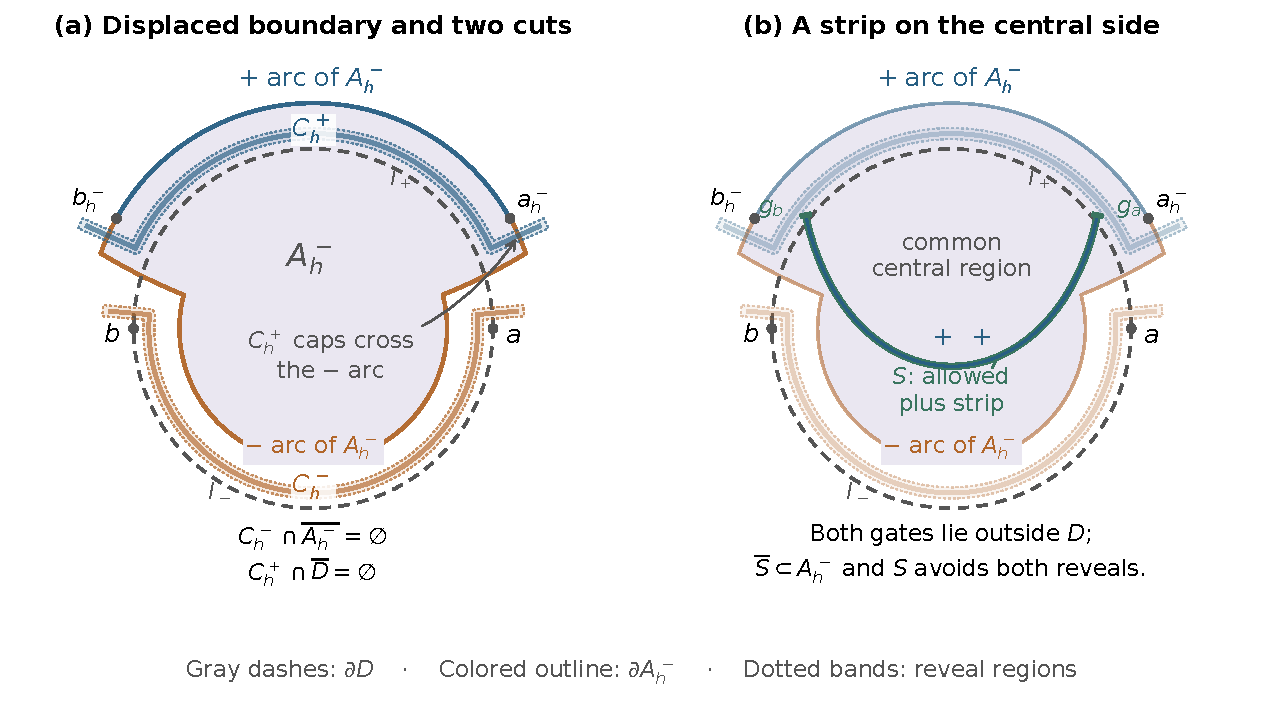
\includegraphics[width=\textwidth]{figures/boundary-squeeze.pdf}
 \caption{Boundary squeeze favoring minus, in fixed Schoenflies
 coordinates.  (a) The dashed circle is $\partial D$; the shaded
 comparison domain has blue plus and orange minus boundary arcs.
 The blue corridor $C_h^+$ lies outside $D$, with caps crossing the
 minus shoulders of $\partial A_h^-$; the orange corridor $C_h^-$ lies
 outside $A_h^-$ and screens the minus arc of $D$.  Dotted bands are
 disjoint reveal regions.  (b) An allowed plus strip $S$ lies on the
 central side of both cuts.  Its gates $g_a,g_b$ are outside $D$, while
 its closure remains inside $A_h^-$ and avoids the reveal regions.
 The thin blue line inside $S$ illustrates a plus spin crossing.
 The drawing shows the preliminary topological configuration; the
 proof uses close polygonal approximations in the physical plane.
 Displacements and widths are schematic.}
 \label{curv:boundary-squeeze}
\end{figure}

The boundary hypothesis in Theorem~\ref{thm:main} is exactly what is
needed here.  If $c$ parametrizes $\partial D$, then $\phi_n\circ c$
converges uniformly to $c$.  Winding numbers therefore determine the
same inside and outside on each compact set disjoint from $\partial D$,
and the marked boundary order gives the same signed-arc incidences away
from the marks.  Fine teeth of $D_n$ remain in a shrinking boundary
collar and cannot enter any of the fixed clearances above.  Virtual
filling records a geometric crossing only: it changes neither a
coupling nor an exterior pin.  The corner check in
\cite[Section~7, paragraph following ``Fixed-geometry boundary
squeeze'']{S} ensures that such a signed path cannot cross the target
resolved contour, including at reflex corners.

\begin{proposition}[Quenched transfer of a finite strip family]
\label{curv:strip-transfer}
Fix $h>0$ and a finite family of allowed plus strips in $A_h^-$.  Let
$\Sigma_{h,n}^-$ have the pure Dobrushin spin law in an ordinary lattice
approximation of $A_h^-$, and let $\Sigma_{n,\omega}$ have the target
spin law.  These samples admit couplings conditional on $\omega$ whose
two marginals are the stated laws and for which
\begin{equation}
 \Prob\!\left(
   \text{every strip crossed by plus in }\Sigma_{h,n}^-
   \text{ is crossed by plus in }\Sigma_{n,\omega}
             \right)=1-o(1).
 \label{curv:strip-order}
\end{equation}
The probability in \eqref{curv:strip-order} includes environment and
coupling randomness.  The pure marginal conditional on $\omega$ is
its deterministic Dobrushin law.  The corresponding assertion holds
for minus strips in $A_h^+$.
\end{proposition}

\begin{proof}
Put the corridors, their reveal regions, and the finitely many strips
inside a torus chart with a fixed positive external buffer.  Choose a
torus period allowed by Proposition~\ref{cross:torus-comparison}.  In
this chart use the same bond environment as the target; complete the
torus with independent bonds.  Write $E_h$ for the event that both
cutting corridors have their prescribed lengthwise colored crossings,
and write $V$ for the vector of ordinary plus crossings of the strips
on the torus.  The pure buffered crossing bounds give
\[
 p_n(E_h)\ge a_h>0,
 \qquad
 p_n=\mathcal L_0(\1_{E_h},V),
\]
for all sufficiently fine meshes.  Here $a_h$ may depend on the fixed
geometry.  With $q_{n,\omega}$ denoting the corresponding quenched
torus vector law, Proposition~\ref{cross:torus-comparison} gives
\begin{equation}
 \E_{\mathrm{env}}\|q_{n,\omega}-p_n\|_{\TV}\longrightarrow0.
 \label{curv:middle-tv}
\end{equation}
At this stage the environmental expectation includes the independently
added torus bonds.

We verify the two order comparisons needed for
Lemma~\ref{curv:conditional-gluing}.  In either torus, conditional on
$E_h$, reveal the prescribed crossing nearest the exterior side of each
corridor.  The stopped reveal of
\cite[Section~6, Lemma ``Reveals with a monochromatic facing boundary'';
Section~7, proof of
``Fixed-geometry boundary squeeze'']{S} leaves only pins of the
prescribed color facing the unrevealed center.  The transcript already
determines crossing existence, so no additional conditioning on $E_h$
remains in that center.  Disjoint reveal regions allow both explorations.

First compare the pure Dobrushin law in $A_h^-$ with the conditioned
pure torus.  The revealed plus path is an upper plus pin against a
lower free spin.  It screens the plus arc of $A_h^-$; every accessible
remaining boundary incidence is a lower minus pin against an upper free
spin.  Meetings of a cut and boundary give upper plus against lower
minus.  The minus reveal is outside $A_h^-$.  Ferromagnetic boundary
comparison therefore puts the pure-domain strip vector below
$p_n(V\in\cdot\mid E_h)$.

Next compare the conditioned random torus, as the lower law, with the
target, as the upper law.  They have identical couplings on every bond
in their common free region.  The minus path screens the target minus
arc.  The remaining boundary incidences, with upper entry first, are
exactly
\[
 (+,\mathrm{free}),\qquad(\mathrm{free},-),\qquad(+,-).
\]
Each comparison follows by conditioning a free spin to its extremal
value and using the nearest-neighbor ferromagnetic order.  This also
explains why no comparison between different random bond strengths is
needed.  The source's geometric incidence check, including the
corridor caps, shows that these are all incidences encountered by the
common components containing the strips.  A nearest-neighbor edge
cannot cross the interior of a separating triangulated diagonal.
Virtual plus values outside $D_n$ give the same order for portions of
a strip that exit and reenter the target.  Thus
$q_{n,\omega}(V\in\cdot\mid E_h)$ is below the target strip vector.

Apply Lemma~\ref{curv:conditional-gluing} with $a=a_h$ and
\eqref{curv:middle-tv}.  It gives \eqref{curv:strip-order}, extending
the strip vectors to the complete spin samples with their conditional
laws.  Finally average over the extra torus bonds while retaining the
original environment.  The conditional pure marginal is unchanged,
and the target marginal never used the extra bonds.  Interchanging
the signs proves the other assertion.
\end{proof}

\subsection{The geometric curve inputs}

For completeness, we state the three further conclusions of the
companion's boundary argument in the form needed here.  Their geometric
parts apply to marked target interfaces with the designated boundary
signs and noncrossing signed barriers; they assume no symmetry of the
target spin law.

\begin{lemma}[Finite strips and limiting barriers]
\label{curv:geometric-input}
For either sign of displacement, the continuum laws
$\mathrm{SLE}_3(A_h^\pm;a_h^\pm,b_h^\pm)$
converge in $d_{\mathrm{curv}}$, as $h\downarrow0$, to
$\mathrm{SLE}_3(D;a,b)$.  Given errors $\eta_j\downarrow0$, one can
choose displacements $h_j\downarrow0$ and, for each $j$, a finite
deterministic family of allowed strips of each sign with the following
property.  Outside an event of pure probability at most $\eta_j$, a
continuum comparison chord selects a strip from its family and traverses
it with strict margins from its long sides and across its end gates.
Only terminal pieces of diameter at most $\eta_j$ are omitted.  The
strip has cross-sections of diameter at most $\eta_j$ following a simple
prototype within $\eta_j$, in $d_{\mathrm{curv}}$, of that middle subarc.
For all sufficiently fine pure lattice approximations, the pure lattice
interface selects such a strip and has the corresponding traversal,
with geometric errors at most $2\eta_j$; its adjacent signed spin path
crosses the strip, outside an event of probability at most $2\eta_j$.

Suppose the prescribed target contours in $D_n$, with their designated
boundary signs, have the corresponding two signed strip barriers with
failure probability tending to zero along such a sequence, and let
$(K,L,U)$ be any joint subsequential limit of their traces and the two
comparison chords, in Hausdorff distance for the traces and
$d_{\mathrm{curv}}$ for the comparison chords.  Here $L$ is the limit
from $A_h^-$ and $U$ the limit from $A_h^+$.  Then almost surely
\begin{equation}
 K\subset\overline{M(L)}\cap\overline{P(U)}.
 \label{curv:forbidden-sides}
\end{equation}
For a simple chord $C$ in $D$, $P(C)$ and $M(C)$ denote the components
of $D\setminus C$ adjacent to $I_+$ and $I_-$; closures are taken in
$\overline D$.
\end{lemma}

\begin{proof}[Source and scope]
The first assertions are
\cite[Section~7, ``From fixed strip tests to limiting barriers'']{S}.
Uniform boundary parametrization gives uniform convergence of the
normalized conformal maps on the closed disk, including the two marks.
Mapping one disk $\mathrm{SLE}_3$ by these maps proves the displaced
continuum convergence.  For fixed $h$, only pure convergence in an
ordinary polygonal approximation is used.

The finite family is obtained by covering favorable simple comparison
chords with open neighborhoods described by rational polygonal strips,
transverse gates, and strict crossing margins.  Compact middle subarcs
are in $D$; the two short terminal pieces tend to the marks.  A
countable such cover has a finite subfamily carrying arbitrarily large
probability.  Its entire list is fixed before taking the lattice limit;
the sampled pure chord may select a strip only after the joint vector
coupling has been made.  Following the signed side of the lattice
interface supplies the crossing with $O(\delta_n)$ drawing error.

The last assertion is the winding and boundary-order argument of
\cite[Section~7, ``Forbidden sides, order, and identification of the
trace'']{S}.  A signed crossing in one of these strips blocks a target
contour from the corresponding side.  To include the open signed
boundary arc, erase loops from the crossing and close it outside $D_n$.
In the fixed $\Psi$ coordinates, take radial connectors from its gates
to a circle $\rho=\rho_*>1$ and the circular arc on the signed side,
where $\rho_*$ is independent of $h,n$.  At fixed $h$, the added path
has positive clearance from $\overline D$ and hence lies outside $D_n$
for large $n$.  Include this threshold in the diagonal choice.  The
target marks are on the zero-winding side of the closed barrier.  As
the strip widths and terminal errors vanish, the gate centers tend
to the marks, while the fixed-radius closure stays a positive distance
beyond every compact subarc of the signed boundary.  The winding
exclusions therefore hold on every compact neighborhood of the
forbidden side or boundary arc, giving
\eqref{curv:forbidden-sides}.  The argument uses only the deterministic
geometry and noncrossing of opposite signed paths with the target
contour; it applies to the couplings in
Proposition~\ref{curv:strip-transfer}.
\end{proof}

\begin{lemma}[Ordered chords with equal laws]
\label{curv:ordered-chords}
Let $L,U$ be random simple chords from $a$ to $b$ with their interiors
in $D$, and let $K\subset\overline D$ be random, compact, connected,
and contain $a,b$.  If \eqref{curv:forbidden-sides} holds almost surely,
then $P(L)\subset P(U)$ almost surely.  If $L$ and $U$ have the same
trace law, then $K=L=U$ as compact sets almost surely.
\end{lemma}

\begin{proof}
This is \cite[Section~7, Lemma ``Ordered chords with equal laws'']{S}.
Here is the argument.  A point of $P(L)\cap M(U)$ could be connected
inside this union to both signed boundary arcs.  Removing loops gives
a crosscut between those arcs that avoids $K$.  Its endpoints
alternate with $a,b$, so it separates $a$ from $b$, contradicting the
connectedness of $K$.  Hence $P(L)\subset P(U)\cup U$.  No point of
$U$ can belong to the open set $P(L)$, since every neighborhood of an
interior point of $U$ meets $M(U)$.  Thus $P(L)\subset P(U)$.

Use a fixed Schoenflies homeomorphism to the disk and take the planar
areas of the images of these two plus sides.  They are bounded, ordered
random variables with the same distribution, so their difference
vanishes almost surely.  If the inclusion of plus sides were proper,
take $z\in P(U)\setminus P(L)$.  It either lies in $M(L)$, or lies on $L$.
In the latter case a neighborhood of $z$ inside $P(U)$ meets $M(L)$,
by the two-sidedness of a Jordan chord.  In either case the difference
contains a nonempty open subset of $M(L)$, and hence has positive area.
The plus sides are therefore equal, and so are their interior boundary
chords.  By \eqref{curv:forbidden-sides}, $K$ lies on this chord.  The
inverse chord parametrization maps it to a connected subset of $[0,1]$
containing both endpoints, which is all of $[0,1]$.
\end{proof}

The remaining issue is traversal order: Hausdorff convergence alone
would allow repeated forward and backward travel close to one simple
chord.  The next source lemma isolates the required exclusion.

\begin{lemma}[Progress criterion for the curve metric]
\label{curv:progress}
Let $g_n$ be simple oriented curves with endpoints tending to $a,b$,
and let $G$ be a continuous injective chord with those endpoints and
interior in $D$.  Suppose their traces converge to the trace of $G$.
There are continuous $u_n:[0,1]\to[0,1]$ with endpoint values tending
to $0,1$ such that
\[
 e_n=\sup_t|g_n(t)-G(u_n(t))|\longrightarrow0.
\]
If $B_n=\sup_{s<t}(u_n(s)-u_n(t))$ tends to zero, then
$d_{\mathrm{curv}}(g_n,G)\to0$.  For each fixed $0<\eta<1$, a drop
$B_n\ge\eta$ instead forces six disjoint passages across an annulus
with center on $G([\eta/2,1-\eta/2])$ and radii $r,R_\eta$, for every
$e_n<r<R_\eta$, once $n$ is sufficiently large; here $R_\eta>0$
depends on $G$ and $\eta$.

Consequently, for random curves coupled with such a random $G$, trace
and endpoint convergence in probability imply curve convergence in
probability if, for every deterministic compact $F\Subset D$ and all
sufficiently small fixed $R>0$,
\begin{equation}
 \lim_{r\downarrow0}\limsup_{n\to\infty}
 \Prob\{\text{$g_n$ has four passages from $r$ to $R$
                  about some center in $F$}\}=0.
 \label{curv:passage-criterion}
\end{equation}
\end{lemma}

\begin{proof}[Source and interpretation]
This is \cite[Section~7, Lemma ``Progress coordinates and the full
curve metric'']{S}, with its passage convention of disjoint parameter
intervals.  Extend the inverse parametrization of $G$ continuously to
an ambient neighborhood and compose it with $g_n$ to obtain $u_n$.
When $B_n\to0$, the running maximum of $u_n$, normalized to endpoint
values $0,1$ and perturbed by a vanishing strictly increasing linear
function, is an increasing homeomorphism uniformly close to $u_n$.
Uniform continuity of $G$ gives the asserted metric convergence.
The other implication is the companion's deterministic passage
argument.  In the random statement, compact exhaustion of $D$ and
deterministic lower bounds on $R_\eta$ on events of increasing
probability reduce its random centers and radii to
\eqref{curv:passage-criterion}.  Six passages imply four, so the latter
condition suffices.  No bound on target path lengths is assumed.
\end{proof}

\subsection{Assembly of the quenched limit}

\begin{proof}[Completion of the proof of Theorem~\ref{thm:main}]
Fix $\epsilon$ in the interval already chosen in
Sections~\ref{sec:crossings} and~\ref{sec:criticality}.  Begin with any
subsequence of the given approximations, and pass further so that the
designation of $I_+$ is fixed.  We will construct, along this
subsequence, deterministic comparison laws $R_n$ and couplings such
that
\begin{equation}
 \mathcal L(L_n\mid\omega)=R_n,\qquad
 \mathcal L(\Gamma_n\mid\omega)=Q_{n,\omega},\qquad
 \E\,\min\{1,d_{\mathrm{curv}}(\Gamma_n,L_n)\}\longrightarrow0,
 \label{curv:quenched-coupling}
\end{equation}
where $R_n\Longrightarrow\mathrm{SLE}_3(D;a,b)$ in the curve metric.

Choose $\eta_j\downarrow0$ and the displacements and finite strip
families of Lemma~\ref{curv:geometric-input}.  For each fixed $j$, apply
Proposition~\ref{curv:strip-transfer} to the two entire families.
Choose increasing deterministic thresholds $n_j$ so that for all
$n\ge n_j$ the geometric placements are valid, the pure comparison
laws have their required approximation bounds, and each strip-transfer
failure probability is at most $\eta_j$.  The threshold may absorb the
reciprocal of $a_{h_j}$ from the conditioning estimate.  Put
\[
 j(n)=\max\{j\le n:n_j\le n\},
\]
with any definition before $n_1$.  This deterministic index tends to
infinity, as slowly as necessary.  Let $L_n$ and $U_n$ be the two pure
comparison chords at displacement $h_{j(n)}$, and denote the law of
$L_n$ by $R_n$.  Their deterministic marginal laws converge to the
same $\mathrm{SLE}_3(D;a,b)$ law.

For each $n$, glue the two strip-transfer couplings over the common
pair $(\omega,\Sigma_{n,\omega})$.  Equivalently, disintegrate each
comparison sample conditional on that pair and then sample both
conditional kernels.  Each comparison marginal conditional on $\omega$
is still its prescribed pure law.  With probability tending to one,
the target has both signed barriers selected from the finite lists
by its two comparison chords.

All target traces lie eventually in one fixed compact planar set.
Indeed uniform boundary convergence bounds $\partial D_n$, and the
bounded components it encloses are bounded by the same large disk.
The space of nonempty compact subsets of this disk is compact in
Hausdorff distance.  The ambient curve space is complete and separable:
rational polygonal paths are dense, and from a Cauchy sequence one can
select a subsequence with successive curve distances less than $2^{-j}$.
Recursively choose parametrizations of its representatives with
successive uniform distances less than $2^{1-j}$.  They converge
uniformly to a continuous path, which represents the limit of the
original Cauchy sequence.  Thus this space is Polish and the usual
weak-convergence and representation theorems apply.  The comparison
chord laws are tight in this space.  Along any further subsequence,
pass again to a joint
limit $(K,L,U)$ of the target trace and comparison chords.  The limit
$K$ is connected, contains $a,b$, and lies in $\overline D$;
connectedness and endpoint inclusion pass under Hausdorff convergence,
and points at positive distance outside $\overline D$ are eventually
outside $D_n$ by the boundary winding argument.  Lemma~\ref{curv:geometric-input}
gives \eqref{curv:forbidden-sides}.  Since $L$ and $U$ have the same
simple chord law, Lemma~\ref{curv:ordered-chords} gives
\[
 K=L=U\qquad\text{almost surely as traces}.
\]

Represent this joint convergence with almost-sure convergence of the
trace and comparison variables, and lift it to the target paths by
their original conditional laws given those variables.  At each mesh the target
configuration space is finite, so this lift is immediate.  It preserves
every target passage probability and requires no prior tightness of
the target paths in the curve metric.  The marginal estimate
Corollary~\ref{cross:four-passages} is precisely
\eqref{curv:passage-criterion} for these target curves, including after
this lift.  Lemma~\ref{curv:progress} therefore gives
$d_{\mathrm{curv}}(\Gamma_n,L)\to0$ in probability in the
representation.  The represented $L_n$ already converges to $L$ in
that metric.  The triangle inequality yields
$d_{\mathrm{curv}}(\Gamma_n,L_n)\to0$ in probability.  This statement
depends only on the joint law of the pair at each $n$, so it holds in
the original couplings as well.  Since every further subsequence
admits this argument, it holds along the whole chosen subsequence.
Boundedness then proves the expectation assertion in
\eqref{curv:quenched-coupling}.

Let $\pi_{n,\omega}$ be the conditional joint law of
$(\Gamma_n,L_n)$ in that coupling, and write
$\overline d=\min\{1,d_{\mathrm{curv}}\}$.  Every function $F$ in the defining
class for $d_{\mathrm{BL}}$ satisfies
\[
 \left|\int F\,\dd Q_{n,\omega}-\int F\,\dd R_n\right|
 \le\int \overline d(\gamma,\ell)\,
                    \dd\pi_{n,\omega}(\gamma,\ell).
\]
The right side is independent of $F$, so taking its supremum and then
environmental expectation gives
\begin{equation}
 \E_{\mathrm{env}}d_{\mathrm{BL}}(Q_{n,\omega},R_n)
 \le \E\,\overline d(\Gamma_n,L_n)\longrightarrow0.
 \label{curv:bl-bound}
\end{equation}
This step uses the conditional pure marginal in
\eqref{curv:quenched-coupling}; its annealed counterpart alone would
not give \eqref{curv:bl-bound}.  The deterministic laws $R_n$ converge
in the same separable curve space to the required SLE law, and hence
their bounded-Lipschitz distances to that law tend to zero.  The
triangle inequality and Markov's inequality prove, for every $\eta>0$,
\[
 \Prob_{\mathrm{env}}\!\left\{
 d_{\mathrm{BL}}\bigl(Q_{n,\omega},\mathrm{SLE}_3(D;a,b)\bigr)
       >\eta\right\}\longrightarrow0
\]
on the chosen subsequence.  If convergence failed on the original
sequence, a subsequence with the displayed probability bounded below
would contradict the construction just given.  This proves the full
sequence assertion.

All couplings used only finitely many bond variables at each mesh;
integrating out added torus bonds and algorithmic variables preserves
the conditional laws given the original infinite environment.  The
bounded-Lipschitz distances are measurable, since $Q_{n,\omega}$ takes
only finitely many values.  Finally restore the prescribed half-stubs
and local drawing.  Their matched displacement is $O(\delta_n)$ and
their orientation remains incoming to outgoing.  Every displacement,
strip, and comparison above was made in the original Euclidean
embedding, and the interval of allowed $\epsilon$ was fixed before
choosing any target geometry.
\end{proof}

\clearpage
\phantomsection
\addcontentsline{toc}{section}{References}
\begin{thebibliography}{99}
\bibitem{AB}
M.~Aizenman and A.~Burchard,
\emph{H\"older regularity and dimension bounds for random curves},
Duke Math. J. \textbf{99} (1999), 419--453.
\href{https://doi.org/10.1215/S0012-7094-99-09914-3}{doi:10.1215/S0012-7094-99-09914-3}.

\bibitem{AW}
M.~Aizenman and J.~Wehr,
\emph{Rounding effects of quenched randomness on first-order phase transitions},
Comm. Math. Phys. \textbf{130} (1990), 489--528.
\href{https://doi.org/10.1007/BF02096933}{doi:10.1007/BF02096933}.

\bibitem{AM}
E.~Av\'erous and R.~Mahfouf,
\emph{The near-critical random bond FK-percolation model},
preprint (2025), \href{https://arxiv.org/abs/2509.08938v1}{arXiv:2509.08938v1}.

\bibitem{BS}
A.~I.~Bugrij and V.~N.~Shadura,
\emph{Duality of a two-dimensional nonhomogeneous Ising model on a finite lattice},
Phys. Rev. B \textbf{55} (1997), 11045--11049.
\href{https://doi.org/10.1103/PhysRevB.55.11045}{doi:10.1103/PhysRevB.55.11045}.
Equation locators refer to the preprint
\emph{Duality of the 2D Nonhomogeneous Ising Model on the Torus},
\href{https://arxiv.org/abs/hep-th/9703037v1}{arXiv:hep-th/9703037v1}.

\bibitem{ChayesShtengel}
L.~Chayes and K.~Shtengel,
\emph{Critical behavior for 2D uniform and disordered ferromagnets at self-dual points},
Comm. Math. Phys. \textbf{204} (1999), 353--366.
\href{https://doi.org/10.1007/s002200050649}{doi:10.1007/s002200050649}.
Theorem locators refer to \href{https://arxiv.org/abs/cond-mat/9811203v1}{arXiv:cond-mat/9811203v1}.

\bibitem{CDHKS}
D.~Chelkak, H.~Duminil-Copin, C.~Hongler, A.~Kemppainen, and S.~Smirnov,
\emph{Convergence of Ising interfaces to Schramm's SLE curves},
C. R. Math. Acad. Sci. Paris \textbf{352} (2014), 157--161.
\href{https://doi.org/10.1016/j.crma.2013.12.002}{doi:10.1016/j.crma.2013.12.002}.
Theorem locators refer to \href{https://arxiv.org/abs/1312.0533v2}{arXiv:1312.0533v2}.

\bibitem{ChelkakSmirnov}
D.~Chelkak and S.~Smirnov,
\emph{Universality in the 2D Ising model and conformal invariance of fermionic observables},
Invent. Math. \textbf{189} (2012), 515--580.
\href{https://doi.org/10.1007/s00222-011-0371-2}{doi:10.1007/s00222-011-0371-2}.

\bibitem{DD}
Vik.~S.~Dotsenko and Vl.~S.~Dotsenko,
\emph{Critical behaviour of the 2D Ising model with impurity bonds},
J. Phys. C: Solid State Phys. \textbf{15} (1982), 495--507.
\href{https://doi.org/10.1088/0022-3719/15/3/015}{doi:10.1088/0022-3719/15/3/015}.

\bibitem{DDReview}
Vik.~S.~Dotsenko and Vl.~S.~Dotsenko,
\emph{Critical behaviour of the phase transition in the 2D Ising model with impurities},
Adv. Phys. \textbf{32} (1983), 129--172.
\href{https://doi.org/10.1080/00018738300101541}{doi:10.1080/00018738300101541}.

\bibitem{DCRT}
H.~Duminil-Copin, A.~Raoufi, and V.~Tassion,
\emph{Sharp phase transition for the random-cluster and Potts models via decision trees},
Ann. of Math. (2) \textbf{189} (2019), 75--99.
\href{https://doi.org/10.4007/annals.2019.189.1.2}{doi:10.4007/\allowbreak annals.2019.189.1.2}.
Locators refer to \href{https://arxiv.org/abs/1705.03104v2}{arXiv:1705.03104v2}.

\bibitem{ES}
R.~G.~Edwards and A.~D.~Sokal,
\emph{Generalization of the Fortuin--Kasteleyn--Swendsen--Wang representation and Monte Carlo algorithm},
Phys. Rev. D \textbf{38} (1988), 2009--2012.
\href{https://doi.org/10.1103/PhysRevD.38.2009}{doi:10.1103/PhysRevD.38.2009}.

\bibitem{FK}
C.~M.~Fortuin and P.~W.~Kasteleyn,
\emph{On the random-cluster model. I. Introduction and relation to other models},
Physica \textbf{57} (1972), 536--564.
\href{https://doi.org/10.1016/0031-8914(72)90045-6}{doi:10.1016/0031-8914(72)90045-6}.

\bibitem{FKG}
C.~M.~Fortuin, P.~W.~Kasteleyn, and J.~Ginibre,
\emph{Correlation inequalities on some partially ordered sets},
Comm. Math. Phys. \textbf{22} (1971), 89--103.
\href{https://doi.org/10.1007/BF01651330}{doi:10.1007/BF01651330}.

\bibitem{GGM}
A.~Giuliani, R.~L.~Greenblatt, and V.~Mastropietro,
\emph{The scaling limit of the energy correlations in non-integrable Ising models},
J. Math. Phys. \textbf{53} (2012), 095214.
\href{https://doi.org/10.1063/1.4745910}{doi:10.1063/1.4745910}.
Theorem locators refer to \href{https://arxiv.org/abs/1204.4040v1}{arXiv:1204.4040v1}.

\bibitem{GP}
R.~L.~Greenblatt and E.~Peltola,
\emph{On the spin interface distribution for non-integrable variants of the two-dimensional Ising model},
preprint (2024), \href{https://arxiv.org/abs/2404.12375v3}{arXiv:2404.12375v3}.

\bibitem{Harris}
A.~B.~Harris,
\emph{Effect of random defects on the critical behaviour of Ising models},
J. Phys. C: Solid State Phys. \textbf{7} (1974), 1671--1692.
\href{https://doi.org/10.1088/0022-3719/7/9/009}{doi:10.1088/0022-3719/7/9/009}.

\bibitem{KS}
A.~Kemppainen and S.~Smirnov,
\emph{Random curves, scaling limits and Loewner evolutions},
Ann. Probab. \textbf{45} (2017), 698--779.
\href{https://doi.org/10.1214/15-AOP1074}{doi:10.1214/15-AOP1074}.

\bibitem{KW}
H.~A.~Kramers and G.~H.~Wannier,
\emph{Statistics of the two-dimensional ferromagnet. Part I},
Phys. Rev. \textbf{60} (1941), 252--262.
\href{https://doi.org/10.1103/PhysRev.60.252}{doi:10.1103/PhysRev.60.252}.

\bibitem{Ludwig}
A.~W.~W.~Ludwig,
\emph{Critical behavior of the two-dimensional random $q$-state Potts model by expansion in $(q-2)$},
Nucl. Phys. B \textbf{285} (1987), 97--142.
\href{https://doi.org/10.1016/0550-3213(87)90330-0}{doi:10.1016/0550-3213(87)90330-0}.

\bibitem{Mahfouf}
R.~Mahfouf,
\emph{The near critical random bond Ising model via embedding deformation},
preprint (2025), \href{https://arxiv.org/abs/2509.08928v1}{arXiv:2509.08928v1}.

\bibitem{OSSS}
R.~O'Donnell, M.~Saks, O.~Schramm, and R.~A.~Servedio,
\emph{Every decision tree has an influential variable},
in Proceedings of the 46th Annual IEEE Symposium on Foundations of Computer Science,
IEEE (2005), 31--39.
\href{https://doi.org/10.1109/SFCS.2005.34}{doi:10.1109/SFCS.2005.34}.

\bibitem{S}
OpenAI,
\emph{$\mathrm{SLE}_3$ universality for weak finite-range Ising interactions},
OpenAI Math Release preprint
\href{https://github.com/openai/math/blob/main/preprints/SLE3-universality-for-weak-finite-range-Ising-interactions-September-23-2026/paper.pdf}{OAI:SLE3-universality-for-weak-finite-range-Ising-interactions-September-23-2026},
2026.

\bibitem{Schramm}
O.~Schramm,
\emph{Scaling limits of loop-erased random walks and uniform spanning trees},
Israel J. Math. \textbf{118} (2000), 221--288.
\href{https://doi.org/10.1007/BF02803524}{doi:10.1007/BF02803524}.

\bibitem{Shalaev}
B.~N.~Shalaev,
\emph{Correlation function and susceptibility of the two-dimensional Ising model with impurities},
Sov. Phys. Solid State \textbf{26} (1984), 1811--1813;
Russian original, Fiz. Tverd. Tela \textbf{26} (1984), 3002--3005.

\bibitem{Shankar}
R.~Shankar,
\emph{Exact critical behavior of a random bond two-dimensional Ising model},
Phys. Rev. Lett. \textbf{58} (1987), 2466--2469;
erratum, \textbf{59} (1987), 380.
\href{https://doi.org/10.1103/PhysRevLett.58.2466}{doi:10.1103/PhysRevLett.58.2466};
\href{https://doi.org/10.1103/PhysRevLett.59.380.2}{doi:10.1103/PhysRevLett.59.380.2}.

\bibitem{SS}
S.~Sheffield and N.~Sun,
\emph{Strong path convergence from Loewner driving function convergence},
Ann. Probab. \textbf{40} (2012), 578--610.
\href{https://doi.org/10.1214/10-AOP627}{doi:10.1214/10-AOP627}.

\bibitem{Smirnov}
S.~Smirnov,
\emph{Conformal invariance in random cluster models. I. Holomorphic fermions in the Ising model},
Ann. of Math. (2) \textbf{172} (2010), 1435--1467.
\href{https://doi.org/10.4007/annals.2010.172.1435}{doi:10.4007/annals.2010.172.1435}.

\end{thebibliography}

\end{document}
